\chapter{Real Analysis}
    When we studied ordered sets we saw that the real numbers possess the
    \textit{least upper bound property}, and could therefore said to be
    complete. In the context of metric spaces we used the notion of Cauchy
    sequences, and then showed that this was equivalent to the nested intervals
    property. There are other equivalent notions, such as the
    Bolzano-Weierstrass theorem and the monotone convergence theorem.
    This property is fundamental to many theorems involved in a standard
    calculus or real analysis course. For example, the concepts of
    differentiation and convergence rely on completeness, and the intermediate
    value theorem may fail without it. On the other hand, $\mathbb{Q}$ is not
    complete. The rationals are, however, \textit{dense} in the reals. That is,
    elements of $\mathbb{R}$ can be approximated arbitrarily well by elements of
    $\mathbb{Q}$. $\mathbb{R}$ is also something called a \textit{field}. From
    algebra, a field is just a set with two operations (Usually called addition
    and multiplication) that are defined in such a way as to give rise to the
    usual notions of addition, subtraction, multiplication, and non-zero
    division, and to give them the basic properties of associativity,
    commutativity, and the distributive law that is found in arithmetic.
    $\mathbb{Q}$ is also a field. Moreover, $\mathbb{R}$ and $\mathbb{Q}$ are
    \textit{ordered fields} with respect to their standard ordering. What makes
    $\mathbb{R}$ special is that it is a complete ordered field. In fact,
    $\mathbb{R}$ is the \textit{only} complete ordered field (Up to
    isomorphism). Completeness in $\mathbb{R}$ can be stated by fact that the
    real numbers have the least upper bound property.
    \begin{definition}
        A bounded above subset of $\mathbb{R}$ is a nonempty subset
        $S\subseteq{\mathbb{R}}$ such that there exists an $M\in\mathbb{R}$ such
        that for all $x\in{S}$, $x\leq{M}$.
    \end{definition}
    \begin{definition}
        An upper bound of a bounded above subset $S\subseteq\mathbb{R}$ is a
        real number $M\in\mathbb{R}$ such that for all $x\in{S}$, $x\leq{M}$.
    \end{definition}
    If $S\subseteq\mathbb{R}$ is bounded above, then there exists infinitely
    many bounds. Completeness says that every bounded above subset has a
    smallest upper bound.
    \begin{theorem}[Least Upper Bound Theorem]
        \label{thm:Func_Least_Upper_Bound_Theorem}%
        If $S\subseteq{\mathbb{R}}$ is bounded above, then there exists an
        $s\in\mathbb{R}$, called the least upper bound, such that $s$ and an
        upper bound and for all upper bounds $M$ of $S$, $s\leq{M}$.
    \end{theorem}
    The proof of Thm.~\ref{thm:Func_Least_Upper_Bound_Theorem} depends on how
    one defines the real numbers. This is often done via Dedekind cuts or
    equivalence classes of Cauchy sequences in $\mathbb{Q}$.
    \begin{theorem}
        There exist bounded above sets $S\subset\mathbb{Q}$ such that for all
        upper bounds $M$ there exists an $s\in\mathbb{Q}$ such that $s$ is an
        upper bound of $S$ and $s<M$.
    \end{theorem}
    \textit{Sketch of Proof.}
    For let $S=\{x\in\mathbb{Q}:x^{2}\leq{2}\}$. This set has no least upper
    bound. Loosely speaking this is because the least upper bound wants to be
    $\sqrt{2}$, but $\sqrt{2}$ is not a rational number. Thus there is no
    rational number to fill the gap.
    \par\hfill\par
    The least upper bound property gives rise
    to many theorems, many of which are equivalent
    to this axiom. Recall that a sequence is a
    function $x:\mathbb{N}\rightarrow{X}$. That is,
    a sequence is a function whose domain is the
    natural numbers, and whose image lies in some
    set $X$. A sequence of real numbers is thus a
    function $x:\mathbb{N}\rightarrow\mathbb{R}$,
    and a sequence of rational numbers is a function
    $x:\mathbb{N}\rightarrow\mathbb{Q}$.
    Often times sequences are denoted $x_{n}$,
    but also the image of $n$ is usually
    denoted $x(n)=x_{n}$ which may be a cause
    for confusion. That is, when we write $x_{n}$
    we often mean $x(n)$, so $x_{0}$, $x_{1}$,
    $x_{2}$ can be written as $x(0)$, $x(1)$,
    $x(2)$ but nobody does this. Similarly,
    we may mean $x_{n}=x$ since nobody writes
    a sequence as $x$. For consistency, we will.
    \begin{definition}
        A sequence in a set $X$ is a function
        $x:\mathbb{N}\rightarrow{X}$.
        We write the image of $n\in\mathbb{N}$
        as $x(n)=x_{n}$.
    \end{definition}
    The notion of \textit{convergence} of a sequence
    in $\mathbb{R}$ is defined as follows.
    \begin{definition}
        A convergent sequence in $S\subseteq\mathbb{R}$
        is a sequence $x:\mathbb{N}\rightarrow{S}$
        such that there exists an $a\in\mathbb{R}$
        such that $|a-x_{n}|\rightarrow{0}$ as
        $n\rightarrow\infty$. We write
        $x_{n}\rightarrow{a}$.
    \end{definition}
    \begin{definition}
        A limit of a sequence $x$
        in a subset $S\subseteq\mathbb{R}$ is an
        element $a\in\mathbb{R}$ such that
        $|a-x_{n}|\rightarrow{0}$.
    \end{definition}
    \begin{theorem}
        If $S\subseteq\mathbb{R}$ and $a$ and $b$ are
        limits of $x:\mathbb{N}\rightarrow{S}$,
        then $a=b$.
    \end{theorem}
    \begin{proof}
        Suppose not. Then $|a-b|>0$. But as $a$ is a
        limit of $x$, there is an $N_{1}\in\mathbb{N}$
        such that, for all $n>N_{1}$,
        $|a-x_{n}|<|a-b|/4$. But, as $b$ is a limit
        of $x$, there is an $N_{2}\in\mathbb{N}$
        such that for all $n>N_{2}$,
        $|b-x_{n}|<|a-b|/4$. Let $N=\max\{N_{1},N_{2}\}+1$.
        But from the triangle inequality:
        $|a-b|\leq|a-x_{N}|+|b-x_{N}|<|a-b|/2$, a
        contradiction. Therefore, $a=b$.
    \end{proof}
    The next notion to discuss is that of
    \textit{subsequences}. There are two ways to define
    a subsequence rigorously. A subsequence of a sequence
    $x:\mathbb{N}\rightarrow{X}$ is a sequence 
    $y:\mathbb{N}\rightarrow{X}$ such that there exists
    a strictly increasing sequence
    $k:\mathbb{N}\rightarrow\mathbb{N}$ such that, for all
    $n\in\mathbb{N}$, $y_{n}=(x\circ{k})(n)$. Here,
    $(x\circ{k})$ is the \textit{composition} of
    the two functions $x$ and $k$. This is
    often written $x_{k_{n}}$, but this can occasionally
    be confusing. We can also just define a subsequence
    to be any strictly increasing sequence
    $k:\mathbb{N}\rightarrow\mathbb{N}$. Given a sequence
    $x:\mathbb{N}\rightarrow{X}$, since $k$ is strictly
    increasing the ordering of $x\circ{k}$
    remains the same, and we've simply skipped over
    some points. Recall that
    monotonic sequences are sequences such
    that, for all $n\in\mathbb{N}$, either
    $x_{n+1}\leq{x_{n}}$ (Monotonically decreasing),
    or $x_{n}\leq{x_{n+1}}$ (Monotonically increasing).
    Strictly monotonic means either $x_{n+1}<x_{n}$
    or $x_{n}<x_{n+1}$ for all $n\in\mathbb{N}$.
    \begin{definition}
        A subsequence is a strictly increasing sequence
        $k:\mathbb{N}\rightarrow\mathbb{N}$
    \end{definition}
    \begin{definition}
        A convergent subsequence of a sequence
        $x:\mathbb{N}\rightarrow{S}$ in
        a subset $S\subseteq\mathbb{R}$ is a
        subsequence $k$ such that
        $x\circ{k}$ is a convergent sequence in $S$.
    \end{definition}
    \begin{definition}
        A monotonic subsequence of a sequence
        $x:\mathbb{N}\rightarrow{S}$ in a subset
        $S\subseteq\mathbb{R}$ is a subsequence
        $k:\mathbb{N}\rightarrow\mathbb{N}$ such
        that $x\circ{k}$ is a monotonic sequence.
    \end{definition}
    \begin{example}
        If $x:\mathbb{N}\rightarrow\mathbb{N}$ is
        the sequence defined by $x_{n}=n$, and if
        $k:\mathbb{N}\rightarrow\mathbb{N}$ is the
        subsequence defined by
        $k_{n}=2n$, then $x_{k_{n}}=2n$. This is the
        subsequence of all even numbers.
        If $k_{n}=2n-1$, then $x_{k_{n}}=2n-1$. This
        is the subsequence of all odd numbers. As a
        boring example, let $k_{n}=n$. Then
        $x_{k_{n}}=n$. This is the identity subsequence.
    \end{example}
    \begin{theorem}
        If $S\subseteq\mathbb{R}$,
        $x:\mathbb{N}\rightarrow\mathbb{R}$ is a
        convergent sequence, and if
        $k:\mathbb{N}\rightarrow\mathbb{N}$ is a
        subequence, then $x\circ{k}$ is a convergent
        sequence.
    \end{theorem}
    \begin{proof}
        For let $\varepsilon>0$.
        As $x$ is a convergent sequence there is
        an $a\in\mathbb{R}$ such that
        $x_{n}\rightarrow{a}$. Thus, there is an
        $N\in\mathbb{N}$ such that, for all
        $n>N$, $|a-x_{n}|<\varepsilon$. But
        $k$ is a subsequence and is therefore
        strictly increasing, so
        for all $n\in\mathbb{N}$, $k_{n}\geq{n}$.
        But then for all $n>N$, $k_{n}>N$, and thus
        $|x_{k_{n}}-a|<\varepsilon$. Therefore,
        $x_{k_{n}}\rightarrow{a}$.
    \end{proof}
    There is an important theorem about
    subsequences of bounded sequences called the
    Bolzano-Weierstrass theorem. It states that
    every bounded sequence has a convergent subsequence,
    and is an equivalent definition of the
    completeness of $\mathbb{R}$. There are a few theorems
    needed before we can prove it.
    \begin{theorem}
        \label{th:funct:bounded_monotone_%
               sequences_converge}
        If $x:\mathbb{N}\rightarrow\mathbb{R}$
        is a bounded monotonic sequence,
        then $x$ is a convergent sequence.
    \end{theorem}
    \begin{proof}
        Let $x$ be a bounded monotonic sequence that
        is increasing in $\mathbb{R}$.
        If $x$ is decreasing, we replace the least
        upper bound with the greatest lower
        bound and the proof is symmetric.
        Then $S=\{x_{n}:n\in\mathbb{N}\}$ is a
        non-empty subset of $\mathbb{R}$. But $x$ is
        a bounded sequence, and therefore $S$ is a
        bounded subset of $\mathbb{R}$. By the least
        upper bound property there exists a least
        upper bound $s\in\mathbb{R}$ of $S$.
        We now show that $x_{n}\rightarrow{s}$.
        Let $\varepsilon>0$ be given. Since $s$ is
        the least upper bound, $s-\varepsilon$
        is not an upper bound of $S$, since
        $s-\varepsilon<s$. Therefore there exists
        an $N\in\mathbb{N}$ such that
        $s-\varepsilon<x_{N}$. But $x$ is
        monotonically increasing, and therefore
        for all $n>N$, $x_{N}\leq{x_{n}}$.
        But, as $s$ is a least upper
        bound of $S$, $x_{n}\leq{s}$. But then,
        for all $n>N$,
        $0\leq{s-x_{n}}\leq{s-x_{N}}<\varepsilon$.
        Therefore, $x_{n}\rightarrow{s}$.
    \end{proof}
    The least upper bound is, in a sense, the
    reason why decimal expansions of
    real numbers work. For example, let $x$ be the
    sequence 3, 3.1, 3.14, 3.141, 3.1415, 3.14159,
    and so forth. This sequence, which is
    the decimal expansion of $\pi$, is bounded by $4$.
    Therefore it has a least upper bound.
    We define the number $\pi$
    to be the least upper bound of this sequence.
    Completeness is a very important property
    but so far it relies on the ordering
    of the real numbers.
    We want to find an equivalent definition
    of completeness that does not rely on ordering
    so that we may speak of complete spaces,
    or sets, which have no notion of
    order. We start with a different definition
    for the completeness of $\mathbb{R}$.
    \begin{definition}
        A Cauchy sequence in a subset
        $S\subseteq\mathbb{R}$ is a
        sequence $x:\mathbb{N}\rightarrow{S}$
        such that for all $\varepsilon>0$ there
        is an $N\in\mathbb{N}$ such that for all
        $n,m>N$, $|x_{n}-x_{m}|<\varepsilon$.
        That is:
        \begin{equation}
            \label{thm:Func_Def_Cauchy_Sequence}
            \forall_{\varepsilon>0}
            \exists_{N\in\mathbb{N}}:
            n,m>N\Rightarrow
            |x_{n}-x_{m}|<\varepsilon
        \end{equation}
    \end{definition}
    \begin{theorem}
        \label{FUNCTIONAL_ANALYSIS:CONVERGENT_%
               SEEQUENCES_ARE_CAUCHY_SEQUENCES}
        If $S\subseteq\mathbb{R}$ and if
        $x:\mathbb{N}\rightarrow{S}$
        is a convergent sequence, then it
        is a Cauchy sequence.
    \end{theorem}
    \begin{proof}
        For let $x$ be a convergent sequence and
        let $a$ be it's limit.
        Let $\varepsilon>0$ be given. Then, as
        $x_{n}\rightarrow{a}$, there is an
        $N\in\mathbb{N}$ such that for all $n>N$,
        $|x_{n}-a|<\varepsilon/2$.
        But by the triangle inequality,
        for all $n,m>N$:
        \begin{equation}
            |x_{n}-x_{m}|\leq
            |x_{n}-a|+|x_{m}-a|<
            \frac{\varepsilon}{2}+
            \frac{\varepsilon}{2}
            =\varepsilon
        \end{equation}
        Therefore, $x$ is a Cauchy sequence.
    \end{proof}
    The converse of
    Thm.~\ref{FUNCTIONAL_ANALYSIS:CONVERGENT_%
              SEEQUENCES_ARE_CAUCHY_SEQUENCES}
    turns out to be a more general notion
    of completeness. That is, we can apply
    this to spaces that do not have
    a notion of order, but do have a notion
    of completeness. There are Cauchy sequences
    $x:\mathbb{N}\rightarrow\mathbb{Q}$ that do
    not converge. This is again related to the fact
    that $\mathbb{Q}$ is not complete. For sequences
    $x:\mathbb{N}\rightarrow\mathbb{R}$,
    if $x$ is Cauchy then it must converge.
    \begin{theorem}
        \label{THM:FUNCTIONAL_ANALYSIS:%
               SUBSEQ_OF_CAUCHY_IS_CAUCHY}
        If $S\subseteq\mathbb{R}$,
        $x:\mathbb{N}\rightarrow{S}$ is a Cauchy sequence,
        and if $k:\mathbb{N}\rightarrow\mathbb{N}$
        is a subsequence, then
        $x\circ{k}$ is a Cauchy sequence.
    \end{theorem}
    \begin{proof}
        For let $\varepsilon>0$. As $x$ is a Cauchy
        sequence, there is an $N\in\mathbb{N}$ such that,
        for all $n,m>N$, $|x_{n}-x_{m}|<\varepsilon$.
        But, as $k$ is a subsequence it is strictly
        increasing, and thus for all $n\in\mathbb{N}$,
        $k_{n}\geq{n}$. But then for all $n,m>N$,
        $k_{n},k_{m}>N$, and thus
        $|x_{k_{n}}-x_{k_{m}}|<\varepsilon$. Thus,
        $x\circ{k}$ is Cauchy.
    \end{proof}
    \begin{theorem}
        If $S\subseteq\mathbb{R}$ and if
        $x:\mathbb{N}\rightarrow{S}$ is a Cauchy sequence,
        then $x$ is a bounded sequence.
    \end{theorem}
    \begin{proof}
        For as $x$ is a Cauchy sequence there is an
        $N\in\mathbb{N}$ such that, for all $n,m>N$,
        $|x_{n}-x_{m}|<1$. Then, for all $n>N+1$,
        $x_{N+1}-1<x_{n}<x_{N+1}+1$. Let
        $M=\max\{|x_{0}|,|x_{1}|,\hdots,|x_{N+1}|+1\}$.
        Then for all $n\in\mathbb{N}$,
        $|x_{n}|\leq{M}$.
    \end{proof}
    We cannot replace the requirement that,
    for all $n,m>N$, $|x_{n}-x_{m}|<\varepsilon$
    with $n,n+k$ for some fixed $k\in\mathbb{N}$.
    There are sequences such that
    $x_{n+1}-x_{n}\rightarrow{0}$,
    yet $x$ is not Cauchy. Indeed, there are such sequences
    that are bounded.
    \begin{example}
        \begin{subequations}
            There are unbounded sequences $x$ such that
            $x_{n+1}-x_{n}\rightarrow{0}$. For let
            $x:\mathbb{N}\rightarrow\mathbb{R}$
            be the sequence defined
            by $x_{n}=\sqrt{n}$. Then:
            \begin{equation}
                |x_{n+1}-x_{n}|=|\sqrt{n+1}-\sqrt{n}|
                =\frac{1}{\sqrt{n+1}+\sqrt{n}}
                <\frac{1}{2\sqrt{n}}
                \rightarrow{0}
            \end{equation}
            But $\sqrt{n}\rightarrow\infty$.
            Moreover, there are bounded sequences $x$
            such that $x_{n+1}-x_{n}\rightarrow{0}$,
            yet $x$ is not Cauchy. For let
            $x:\mathbb{N}\rightarrow\mathbb{R}$
            be defined by
            $x_{n}=\cos(\pi\sqrt{n})$.
            Then $x$ is bounded, and:
            \begin{align}
                x_{n+1}-x_{n}
                &=\cos\big(\pi\sqrt{n+1})
                    -\cos(\pi\sqrt{n}\big)\\
                &=-2\sin\Big(\pi
                    \frac{\sqrt{n+1}-\sqrt{n}}{2}\Big)
                    \sin\Big(\pi
                        \frac{\sqrt{n+1}+\sqrt{n}}{2}\Big)
            \end{align}
            But we saw from the previous example that
            $\sqrt{n+1}-\sqrt{n}\rightarrow{0}$, and
            therefore $x_{n+1}-x_{n}\rightarrow{0}$.
            $x$ is not Cauchy, however, for let
            $k:\mathbb{N}\rightarrow\mathbb{N}$ be
            the subsequence defined by $k_{n}=n^{2}$. Then:
            \begin{equation}
                x_{k_{n}}=\cos(\pi{n})=(-1)^{n}
            \end{equation}
            And this is not a Cauchy sequence. By
            Thm.~\ref{THM:FUNCTIONAL_ANALYSIS:%
                      SUBSEQ_OF_CAUCHY_IS_CAUCHY},
            $x$ is not a Cauchy sequence.
        \end{subequations}
    \end{example}
    \begin{theorem}
        \label{th:funct:sequences_have_%
               monotonic_subsequence}
        Every sequence in $\mathbb{R}$
        has a monotonic subsequence.
    \end{theorem}
    \begin{proof}
        Let $x$ be a sequence in $\mathbb{R}$.
        Call $n$ a ``peak point'' if
        $x_{n}\geq{x_{m}}$ for all
        ${m}\geq{n}$. If there are infinitely many
        of these peak points, then we have obtained
        a decreasing sequence, since the $n^{th}$
        peak point will be greater than or equal to
        the $(n+1)^{th}$ peak point.
        We have thus obtained
        a monotonically decreasing subsequence.
        If there are finitely many,
        there are either zero or there is a last one,
        $x_{n_{0}}$. Then $x_{n_{0}+1}$ is not a
        peak point. But then there is a
        $k\in\mathbb{N}$ such that $k>n_{0}+1$ and
        $x_{k}\geq{x_{n_{0}+1}}$, for otherwise
        $x_{n_{0}+1}$ would be a peak point. But
        $x_{k}$ is also not a peak point, and so
        there is a $k_{1}$ such that $k_{1}>k$ and
        $x_{k_{1}}\geq{x_{k}}$. This pattern
        continues, and we thus have a monotonically
        increasing subsequence. If there are zero
        peak points, repeat the argument above
        argument with $x_{n_{0}}=x_{1}$.
    \end{proof}
    There's probably some axiom of choice stuff
    going on here.
    \begin{theorem}[Bolzano-Weierstrass Theorem]
        If $x:\mathbb{N}\rightarrow\mathbb{R}$
        is a bounded sequence, then there is
        a convergent subsequence
        $k:\mathbb{N}\rightarrow\mathbb{N}$
        of $x$.
    \end{theorem}
    \begin{proof}
        By Thm.~\ref{th:funct:sequences_%
                     have_monotonic_subsequence},
        if $x:\mathbb{N}\rightarrow\mathbb{R}$ is a
        sequence, then there is a monotonic subsequence
        $k:\mathbb{N}\rightarrow\mathbb{N}$.
        But by Thm.~\ref{th:funct:bounded_%
                         monotone_sequences_converge},
        bounded monotonic sequences converge.
        Thus $x\circ{k}$ converges.
        Therefore $k$ is a convergent
        subsequence of $x$.
    \end{proof}
    This notion is so important it has a name.
    A sequentially compact space is a space such that
    every sequence has a convergent subsequence. The
    Bolzano-Weierstrass Theorem is equivalent
    to saying that every closed and bounded subset
    of $\mathbb{R}$ is sequentially
    compact. The general notion of \textit{compactness}
    is a topological one, but as it turns out
    sequential compactness and compactness are
    identical concepts in a \textit{metric space}.
    Metric spaces will be one of the primary
    subjects of study in functional analysis.
    In $\mathbb{R}^{n}$ there is another equivalent,
    and perhaps more intuitive,
    definition of compactness. A subset of
    $\mathbb{R}^{n}$ is compact if and only if it
    is closed and bounded. A set
    $S\subseteq\mathbb{R}$ is closed if for
    all convergent sequences
    $x:\mathbb{N}\rightarrow{S}$,
    the limit also lies in $S$.
    Compactness will be discussed later in the
    context of continuous functions on a compact set.
    \begin{example}
        \begin{subequations}
            Find a subsequence $k$ of the identity
            $x:\mathbb{N}\rightarrow\mathbb{R}$
            defined by $x_{n}=n$ for which
            both $\sin(x\circ{k})$ and $\cos(x\circ{k})$
            converge. First note that for any subsequence
            $k$, $(x\circ{k})(n)=k_{n}$.
            In degrees this is simple:
            \begin{equation}
                k_{n}=360n+45
                \Rightarrow
                \sin(k_{n})=\cos(k_{n})
                =\frac{1}{\sqrt{2}}
            \end{equation}
            In radians we need to be a little more careful.
            Let $y:\mathbb{N}\rightarrow\mathbb{R}$
            be defined by $y_{n}=\sin(n)$.
            Then $y$ is bounded and
            by the Bolzano-Weierstrass theorem,
            there is a convergent subsequence $k$.
            Let $z:\mathbb{N}\rightarrow\mathbb{R}$
            be defined by $z_{n}=\cos(k_{n})$. Then $z$
            is bounded and by the
            Bolzano-Weierstrass theorem there is a
            convergent subsequence $j$. Let $k_{j}$
            denote the subsequence $k\circ{j}$. But
            any subsequequence of a convergent sequence
            converges to the same limit, and therefore
            $\sin(k_{j})$ is a convergent sequence. Thus,
            $\sin(k_{j})$ and $\cos(k_{j})$ are
            convergent sequences. It's also
            possible to make them converge to the same
            limit. We need to know that
            $\{n\mod\alpha:n\in\mathbb{N}\}$ is dense
            in $(0,\alpha)$ when $\alpha$ is irrational.
            Thus there is a subsequence such that
            $k_{n}\mod2\pi\rightarrow\pi/4$.
            Then $\sin(k_{n})$ and $\cos(k_{n})$
            both converge to $1/\sqrt{2}$.
            Let's first try to find a subsequence such that
            $\cos(k_{n})\rightarrow{1}$. If we can
            do that, we simply need to modify the
            argument so that
            $\cos(k_{n})\rightarrow{1}/\sqrt{2}$.
            Let $k$ be a sequence of integers
            such that $0<n-2\pi{k_{n}}<2\pi$.
            Let $\varepsilon>0$ and let $N\in\mathbb{N}$
            be such that $N>\frac{2\pi}{\varepsilon}$.
            Now consider the set:
            \begin{equation}
                A_{N}=\{n-2\pi{k_{n}}:n=1,2,\hdots,N+1\}
            \end{equation}
            Then $A_{N}$ has $N+1$ elements and by the
            pidgeon-hole principle there are
            elements that are within
            $2\pi/\frac{2\pi}{\varepsilon}$ of each other.
            Let $n_{1}$ and $n_{2}$ be such numbers.
            Then:
            \begin{align}
                \cos(n_{2}-n_{1})
                &=\cos(n_{2}-n_{1}-2\pi(k_{2}-k_{1}))\\
                &=\cos((n_{2}-2\pi{k}_{2})
                       -(n_{1}-2\pi{k_{1}}))\\
                &=\cos(\xi)
            \end{align}
            Where $\xi$ is a number such that
            $0<|\xi|<\varepsilon$. But then
            $|1-\cos(\xi)|<\frac{\varepsilon^{2}}{2}$.
            And $n_{2}-n_{1}$ is a natural number,
            so we can find a subsequence $k$ such
            that $\cos(k_{n})\rightarrow{1}$. Modifying
            this with $\pi/4$
            and $1/\sqrt{2}$ gives the result.
        \end{subequations}
    \end{example}
    \begin{theorem}
        If $x:\mathbb{N}\rightarrow\mathbb{R}$ is
        a Cauchy sequence, then it converges.
    \end{theorem}
    \begin{proof}
        If $x$ is Cauchy, then it is bounded.
        By the Bolzano-Weiestrass theorem there
        is a convergent subsequence $k$. But then there
        is an $a\in\mathbb{R}$ such that
        $x_{k_{n}}\rightarrow{a}$. We now must show that
        $x_{n}\rightarrow{a}$. Let $\varepsilon>0$
        be given. As $x_{k_{n}}\rightarrow{a}$,
        there is an $N_{1}\in\mathbb{N}$ such
        that for all $n>N_{1}$,
        $|x_{k_{n}}-a|<\frac{\varepsilon}{2}$.
        But as $x$ is a Cauchy sequence, there
        is an $N_{2}$ such that for all $n,m>N_{2}$, 
        $|x_{n}-x_{m}|<\frac{\varepsilon}{2}$. Let
        $N=\max\{N_{1},N_{2}\}$. 
        But $k$ is a subsequence, and thus for all
        $n>N$, $k_{n}>N$. But then if $n>N$,
        $|x_{k_{n}}-x_{n}|<\frac{\varepsilon}{2}$.
        By the triangle inequality,
            $|a-x_{n}|\leq
             |a-x_{k_{n}}|+|x_{k_{n}}-x_{n}|\leq
             \frac{\varepsilon}{2}+
             \frac{\varepsilon}{2}%
             =\varepsilon$.
    \end{proof}
    Real numbers can be constructed by considering
    \textit{equivalence classes} of Cauchy sequences of
    rational numbers. Two Cauchy sequences $x_{n}$ and
    $y_{n}$ are equivalent if $x_{n}-y_{n}\rightarrow{0}$.
    By considering the set
    of all such equivalent sequences, we can give a more
    rigorous construction of the real numbers.
    \begin{example}
        \begin{subequations}
            Let $x:\mathbb{N}\rightarrow\mathbb{Q}$
            be the sequence:
            \begin{equation}
                x_{n}=\frac{2n+3}{n}
            \end{equation}
            Let $\varepsilon>0$ and let
            $N=\ceil{6/\varepsilon}+1$.
            Then, for $n,m>N$, we have:
            \begin{equation}
                |x_{n}-x_{m}|=
                \Big|\frac{2n+3}{n}-\frac{2m+3}{m}\Big|
                =3\Big|\frac{n-m}{nm}\Big|
                <\frac{6}{\min\{n,m\}}
                <\frac{6}{N}<\varepsilon
            \end{equation}
            Therefore $x$ is a Cauchy sequence of rational
            numbers. It has a standard representation
            of 2 since $x_{n}\rightarrow{2}$. To see this:
            \begin{equation}
                \Big|2-\frac{2n+3}{n}\Big|
                =\Big|\frac{3}{n}\Big|\rightarrow{0}
            \end{equation}
            There are other elements of the equivalence
            class for 2. Indeed the sequence
            $x:\mathbb{N}\rightarrow\mathbb{Q}$ defined
            by $x_{n}=2$ for all $n\in\mathbb{N}$ is
            such an example. The equivalence classes
            also define the irrational numbers as well.
            For let $x:\mathbb{N}\rightarrow\mathbb{Q}$
            be defined by:
            \begin{equation}
                x_{n}=\sum_{k=0}^{n}\frac{(-1)^{k}}{n!}
            \end{equation}
            The ratio test, or the alternating series
            test, can be applied to show that this
            converges. Convergent sequences are Cauchy
            sequence, and thus $x$ can be used to
            represent some real number. The number it
            represents is $e^{-1}$, which is irrational.
            If one recalls the history of $e$, we know
            that the equivalence class for $e^{-1}$ also
            contains the following sequence:
            \begin{equation}
                x_{n}=\Big(1-\frac{1}{n}\Big)^{n}
            \end{equation}
        \end{subequations}
    \end{example}
    We have seen that the least upper bound axiom,
    together with the ordered field structure that
    $\mathbb{R}$ possesses, implies that
    Cauchy sequence in $\mathbb{R}$ converge. This can
    be reversed, showing that we now have two equivalent
    definitions of completeness.
    \begin{theorem}
        If $x:\mathbb{N}\rightarrow\mathbb{R}$
        is a bounded monotonic sequence, then
        $x$ is a Cauchy sequence.
    \end{theorem}
    \begin{proof}
        For suppose not. Suppose $x$ is monotonically
        increasing. If $x$ is not Cauchy
        then there exists an $\varepsilon>0$ such
        that, for all $N\in\mathbb{N}$ there exists
        $n,m>N$ such that
        $|x_{n}-x_{m}|\geq\varepsilon$. But if
        $x$ is bounded, there is an $s$ such that,
        for all $n\in\mathbb{N}$, $|x_{n}|\leq{s}$.
        From the Archimedean principle, as
        $\varepsilon>0$ there is an $N_{1}\in\mathbb{N}$
        such that $x_{1}+N_{1}\varepsilon>s$.
        Let $X=\{x_{n}:n\in\mathbb{N}\}$.
        For all $N\in\mathbb{N}$, $N\geq{2}$,
        there exists a function
        $z:\mathbb{Z}_{N}\rightarrow{X}$ such that, for
        all $n\in\mathbb{Z}_{N-1}$,
        $z_{n}<z_{n+1}$, and
        $\min(\{|z_{n}-z_{m}|:n,m\in\mathbb{Z}_{N}\})%
         \geq\varepsilon$. By induction,
        let $z_{1}=x_{1}$. As $x$ is not Cauchy, there
        are $n,m>1$ such that
        $|x_{n}-x_{m}|\geq\varepsilon$. But from
        monotonicity, $x_{m}\geq{x}_{1}$, and thus
        $|x_{n}-x_{1}|\geq\varepsilon$.
        Let $z_{2}=x_{n}$. Suppose it is true for
        $N\in\mathbb{N}$. Let
        $z:\mathbb{Z}_{N}\rightarrow{X}$ be such a
        function. As $x$ is not Cauchy and
        monotonic, there is an $n>N$ such that
        $|x_{n}-z_{N}|\geq\varepsilon$.
        Let $z':\mathbb{Z}_{N+1}\rightarrow{X}$
        be defined by:
        \begin{subequations}
            \begin{equation}
                z'_{k}=
                \begin{cases}
                    z_{k},&1\leq{k}\leq{N}\\
                    x_{n},&k=N+1
                \end{cases}
            \end{equation}
            From monotonicity, for all
            $n\in\mathbb{Z}_{N}$,
            $z'_{N+1}-z'_{n}\geq\varepsilon$. Moreover,
            $z'_{N+1}>z'_{N}$. Thus $z'$
            satisfies the criterion.
            Thus, there is a function
            $z:\mathbb{Z}_{N_{1}+1}\rightarrow{X}$
            such that $z$ is increasing and
            $\min(\{|z_{n}-z_{m}|:%
                    n,m\in\mathbb{Z}_{N_{1}}\})%
             \geq\varepsilon$.
             But then:
            \begin{equation}
                z_{N_{1}+1}-z_{1}=
                \sum_{n=1}^{N_{1}}(z_{n+1}-z_{n})
                \geq{N}_{1}\varepsilon
            \end{equation}
            But then:
            \begin{equation}
                z_{N_{1}+1}>z_{1}+N_{1}\varepsilon
            \end{equation}
            But $z_{1}\in{X}$, and thus
            $z_{1}\geq{x}_{1}$. But then
            $z_{N_{1}+1}>x_{1}+N\varepsilon$. But
            $s<x_{1}+N\varepsilon$, a contradiction
            as $s\geq{x}_{n}$ for all $n\in\mathbb{N}$.
            Therefore, $x$ is Cauchy.
        \end{subequations}
    \end{proof}
    This shows that the monotone convergence theorem
    can be proved without the least upper bound principle.
    The proof becomes messier, however. We now prove
    the equivalence of completeness and the least upper
    bound axiom.
    \begin{theorem}
        If every Cauchy sequence in $\mathbb{R}$
        is a convergent sequence, then every
        bounded above subset of $\mathbb{R}$ has a
        least upper bound.
    \end{theorem}
    \begin{proof}
        For if $L\subseteq\mathbb{R}$ is non-empty and
        bounded then there is an $a\in{L}$ and an
        $s\in\mathbb{R}$ such that, for all
        $y\in{L}$, $y\leq{s}$. If $s\in{L}$, then
        $s$ is a least upper bound of $L$. Suppose not.
        Let
        $S=\{y\in\mathbb{R}:\forall_{x\in{L}}x\leq{y}\}$.
        Then $S$ is non-empty, as $s\in{S}$.
        Suppose $s$ is not the least upper bound of $L$
        and define the following:
        \begin{subequations}
            \begin{equation}
                A_{k}
                =\Big\{s-\frac{n}{2^{k}}:
                       n\in\mathbb{N}\Big\}
                \bigcap{S}
            \end{equation}
            There exists an $N\in\mathbb{N}$ such that, for
            all $k>N$, $A_{k}\ne\emptyset$, for otherwise
            $s$ would be a least upper bound. Moreover, for
            all $k>N$, $A_{k}$ is finite for by the
            Archimedean property there is an
            $n\in\mathbb{N}$ such that $s-n/2^{k}<x$,
            and thus for all $m>n$,
            $s-m/2^{k}\notin{A_{k}}$.
            Lastly, $A_{k}\subseteq{A_{k+1}}$. Let
            $x:\mathbb{N}\rightarrow\mathbb{R}$
            be defined by:
            \begin{equation}
                x_{n}=\min(A_{n+N})
            \end{equation}
        \end{subequations}
        This is well defined since, for all
        $n>N$, $A_{n}$ is finite. Then, since
        $A_{n}\subseteq{A_{n+1}}$ for all
        $n>N$, $x$ is a monotonically decreasing
        sequence. But then $x$ is monotonic and
        bounded, and is therefore Cauchy. But Cauchy
        sequences converge, and thus there is a
        $c\in\mathbb{R}$ such that
        $x_{n}\rightarrow{c}$. For all $y\in{L}$,
        $y\leq{c}$. For if there is a
        $y\in{L}$ such that $c<y$, then there is an
        $N$ such that $x_{N}<y$, a contradiction as
        $x_{N}\in{S}$. Thus, $c$ is an upper bound of $L$.
        Suppose $c$ is not
        the least upper bound, and thus there is a
        $d\in{S}$ such that $d<c$. But then there is an
        $k\in\mathbb{N}$ such that $c-d<2^{-k}$. But
        then $x_{k+1}<c$, a contradiction as $x$
        is monotonically decreasing and
        $x_{n}\rightarrow{c}$. Thus, $c$ is the least
        upper bound.
    \end{proof}
    We've now used the Archimedean property twice. This
    says that for any $\varepsilon>0$ and any
    $x>0$, there is an $N\in\mathbb{N}$ such that
    $N\varepsilon>x$. It is equivalent to saying the
    real numbers have no ``infinitesimals.'' We now
    have two ways to talk about the completeness of
    $\mathbb{R}$. The monotone convergence theorem
    can also be taken as axiom, and shown that it
    implies completeness, as well as the
    Bolzano-Weierstrass theorem. Lastly, there is the
    Nested Interval Theorem which will be proved later
    in the context of more general metric spaces.
    \section{Old stuff}
        \subsection{Continuity}
            We now discuss continuity, uniform continuity, and
            related theorems.
            \begin{definition}
                A function $f:S\rightarrow\mathbb{R}$
                on a subset $S\subseteq\mathbb{R}$ continuous
                at a point $x\in{S}$ is a function such that
                for all $\varepsilon>0$ there is a $\delta>0$
                such that for all $x_{0}\in{S}$,
                $|x-x_{0}|<\delta$ implies
                $|f(x)-f(x_{0})|<\varepsilon$. That is:
                \begin{equation}
                    \forall_{\varepsilon>0}\exists_{\delta>0}:
                    x\in{S},|x-x_{0}|<\delta
                    \Rightarrow|f(x)-f(x_{0})|<\varepsilon
                \end{equation}
            \end{definition}
            \begin{theorem}
                If $S\subseteq\mathbb{R}$, $x\in{S}$,
                $f:S\rightarrow\mathbb{R}$
                is continuous at $x$, and if
                $a:\mathbb{N}\rightarrow{S}$
                is a convergent sequence such that
                $a_{n}\rightarrow{x}$, then
                $f(a_{n})\rightarrow{f(x)}$.
            \end{theorem}
            \begin{proof}
                For let $\varepsilon>0$. As $f$ is
                continuous there is a $\delta>0$ such that,
                for all $x_{0}\in{S}$
                such that $|x-x_{0}|<\delta$,
                $|f(x)-f(x_{0})|<\varepsilon$.
                But $a_{n}\rightarrow{x}$, and thus there is an
                $N\in\mathbb{N}$ such that, for all $n>N$,
                $|x-a_{n}|<\delta$. But then, for all $n>N$,
                $|f(x)-f(a_{n})|<\varepsilon$. Therefore,
                $f(a_{n})\rightarrow{f(x)}$.
            \end{proof}
            The converse of this theorem is true, giving us
            an equivalent definition of continuity.
            \begin{theorem}
                If $S\subseteq\mathbb{R}$, $x\in{S}$ and
                $f:S\rightarrow\mathbb{R}$
                is a function such that for all sequences
                $a:\mathbb{N}\rightarrow\mathbb{R}$ such that
                $a_{n}\rightarrow{x}$,
                $f(a_{n})\rightarrow{f(x)}$,
                then $f$ is continuous at $x$.
            \end{theorem}
            \begin{proof}
                For suppose not. Then there is an
                $\varepsilon>0$ such that, for all $\delta>0$,
                there is an $x_{0}\in{S}$ such that
                $|x-x_{0}|<\delta$ and
                $|f(x)-f(x_{0})|\geq\varepsilon$.
                Let $a:\mathbb{N}\rightarrow\mathbb{R}$
                be a sequence such that, for all
                $n\in\mathbb{N}$, $|a_{n}-x|<1/n$, but
                $|f(x)-f(a_{n})|\geq\varepsilon$.
                But then $a_{n}\rightarrow{x}$. But for all
                sequences $a$ such that $a_{n}\rightarrow{x}$,
                $f(a_{n})\rightarrow{f(x)}$. But, for all $n$,
                $|f(x)-f(a_{n})|\geq\varepsilon$,
                a contradiction.
                Therefore, $f$ is continuous at $x$.
            \end{proof}
            \begin{theorem}
                If $x\in\mathbb{R}$ and
                $a:\mathbb{N}\rightarrow\mathbb{R}$
                is a convergent sequence such that
                $a_{n}\rightarrow{x}$ and for all
                $n\in\mathbb{N}$, $a_{n}\geq{0}$,
                then $x\geq{0}$.
            \end{theorem}
            \begin{proof}
                For suppose not. Suppose $x<0$. Let
                $\varepsilon=|x|/2$. Then, as $\varepsilon>0$, there
                is an $N\in\mathbb{N}$ such that for all $n>N$,
                $|x-a_{n}|<\varepsilon$. But then
                $a_{N+1}<x+\varepsilon=x/2<0$, a contradiction as
                $a_{N+1}\geq{0}$.
            \end{proof}
            \begin{theorem}
                \label{thm:Funct:Continuous_Limit_%
                       of_Pos_Sequ_is_nonneg}
                If $S\subseteq\mathbb{R}$, $x\in{S}$,
                $f:S\rightarrow\mathbb{R}$ is continuous at $x$, and if
                $a:\mathbb{N}\rightarrow\mathbb{R}$ is a sequence such
                that  $a_{n}\rightarrow{x}$ and $f(a_{n})>0$
                for all $n\in\mathbb{N}$, then $f(x)\geq{0}$.
            \end{theorem}
            \begin{proof}
                For suppose not. Let $r=f(x)<0$, and let
                $\varepsilon=|r|/2$. Then $\varepsilon>0$. But
                from continuity, there is a $\delta>0$ such that
                for all $x_{0}\in{S}$ such that $|x-x_{0}|<\delta$,
                $|f(x)-f(x_{0})|<\varepsilon$. But
                $a_{n}\rightarrow{x}$, and thus there is an
                $N\in\mathbb{N}$ such that for all $n>N$,
                $|x-a_{n}|<\delta$. Thus
                $|f(x)-f(a_{N+1})|<\varepsilon$. But then
                $f(a_{n})<f(x)+\varepsilon=f(x)/2<0$,
                a contradiction as $f(a_{N+1})>0$. Therefore, etc.
            \end{proof}
            \begin{theorem}
                If $x\in\mathbb{R}$,
                $f:\mathbb{R}\rightarrow\mathbb{R}$ is
                continuous at $x$, and if $f(x)>0$,
                then there is an open interval
                $\mathcal{U}$ such that $x\in\mathcal{U}$,
                and for all $y\in\mathcal{U}$, $f(y)>0$.
            \end{theorem}
            \begin{proof}
                For let $\varepsilon=f(x)/2$. Then
                $\varepsilon>0$, and thus there is a $\delta>0$
                such that for all $x_{0}\in\mathbb{R}$
                such that $|x-x_{0}|<\delta$,
                $|f(x)-f(x_{0})|<\varepsilon$. Let
                $\mathcal{U}=(x-\delta,x+\delta)$.
                Then $\mathcal{U}$ is an open intervals and if
                $y\in\mathcal{U}$, then $|x-y|<\delta$,
                and therefore:
                \begin{equation}
                    |f(y)-f(x)|<\varepsilon
                    \Rightarrow
                    f(y)>f(x)-\varepsilon
                    =\frac{f(x)}{2}>0
                \end{equation}
                Thus, for all $y\in\mathcal{U}$, $f(y)>0$.
            \end{proof}
            \begin{definition}
                A continuous function on
                $S\subseteq\mathbb{R}$ is a function
                $f:S\rightarrow\mathbb{R}$ such that
                $f$ is continuous at all $x\in{S}$. That is:
                \begin{equation}
                    \forall_{x\in{S}}\forall_{\varepsilon>0}
                    \exists_{\delta>0}:x_{0}\in{S},
                    |x-x_{0}|<\delta
                    \Rightarrow|f(x)-f(x_{0})|<\varepsilon
                \end{equation}
            \end{definition}
            This definition comes from the fact that
            continuity is a point-wise property, and not a
            ``curve'' property. Continuous functions are
            functions that have point-wise continuity at
            every point. The statement ``A continuous function
            is a curve that you can draw,'' which many have
            heard in calculus, is slightly misleading. There
            are functions that are continuous at one point and
            nowhere else. There are functions that are
            continuous on the irrationals and discontinuous
            on the rationals. For example, if $x$ is
            rational write it as $x=p/q$ where $p$ and
            $q$ are integers and relatively prime. Define $f$
            as follows:
            \begin{equation}
                f(x)=
                \begin{cases}
                    \frac{1}{q},&x\in\mathbb{Q}\\
                    0,&x\notin\mathbb{Q}
                \end{cases}
            \end{equation}
            This function, which is known as Dirichlet's Function, but also as
            the Popcorn Function, or Thomae's Function, is continuous at every
            irrational number and discontinuous at every rational number.
            \begin{figure}[H]
                \captionsetup{type=figure}
                \centering
                \documentclass[crop,class=article]{standalone}
%----------------------------Preamble-------------------------------%
\usepackage{tikz}                       % Drawing/graphing tools.
\usetikzlibrary{arrows.meta}            % Latex arrows.
%--------------------------Main Document----------------------------%
\begin{document}
    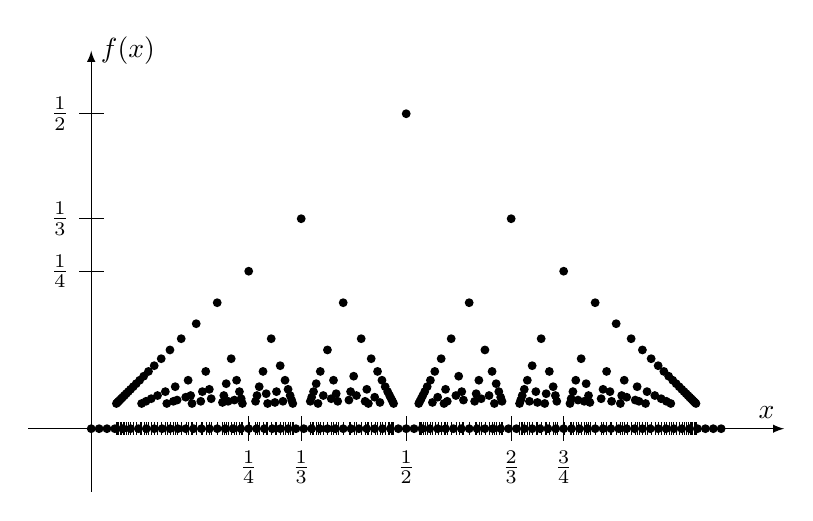
\begin{tikzpicture}[scale=8,>=latex]
        \draw[->] (-0.1,0) -- (1.1,0)
            node[above left] {$x$};
        \draw[->] (0,-0.1) -- (0,0.6)
            node[right] {$f(x)$};
        \draw (0.02,1/2) -- (-0.02,1/2)
            node[left]{$\frac{1}{2}$};
        \draw (0.02,1/3) -- (-0.02,1/3)
            node[left]{$\frac{1}{3}$};
        \draw (0.02,1/4) -- (-0.02,1/4)
            node[left]{$\frac{1}{4}$};
        \foreach\X[%
            evaluate=\X as \Ymax using {int(\X-1)}]
            in {25,24,...,2}{%
                \foreach\Y in {1,...,\Ymax}{%
                    \ifnum\X<5
                        \draw
                        (\Y/\X,0.02) -- (\Y/\X,-0.02)
                        node[below,fill=white]
                            {$\frac{\Y}{\X}$};
                    \else
                        \draw[ultra thin]
                        (\Y/\X,0.01) to (\Y/\X,-0.01);
                    \fi
                    \pgfmathtruncatemacro{\TST}
                        {gcd(\X,\Y)}
                    \ifnum\TST=1
                        \fill ({\Y/\X},1/\X) 
                            circle (0.2pt); 
                    \fi
                }
        }
        \foreach\X in {0,1,...,80}
        {\fill (\X/80,0) circle(0.2pt);}
    \end{tikzpicture}
\end{document}
                \caption{Dirichlet's Popcorn Function}
                \label{fig:Dirichlet_Thomae_Function}
            \end{figure}
            There is no ``reverse,'' of this
            function. That is, there is no function which is
            continuous on $\mathbb{Q}$ and discontinuous at
            every irrational number. Uniform continuity is a
            property of all points in the domain of a function.
            Point-wise continuity says that given a point $x$
            and a positive number
            $\varepsilon$, one can find a $\delta$ satisfying a
            certain property. The key part is that the point $x$ must
            be specified first. That is, the $\delta$
            may be dependent on $x$.
            Uniform continuity occurs when a $\delta>0$ can be
            chosen regardless of $x$. $\delta$ is
            only dependent on $\varepsilon$.
            \begin{definition}
                A uniformly continuous function on a subset
                $S\subseteq\mathbb{R}$
                is a function $f:S\rightarrow\mathbb{R}$ such that:
                \begin{equation*}
                    \forall_{\varepsilon>0}\exists_{\delta>0}
                    \forall_{x\in{S}}:\forall_{x_{0}\in{S}},
                    |x-x_{0}|<\delta
                    \Rightarrow|f(x)-f(x_{0})|<\varepsilon    
                \end{equation*}
            \end{definition}
            Continuity is a point-wise property. There are
            functions that are continuous at one point
            and nowhere else. Uniform continuity, however,
            is a set property. You can't have uniform
            continuity at a single point,
            but rather on a set of points. Unless, of course,
            your domain $S$ is a single point. But that's rather boring.
            \begin{theorem}
                \label{thm:Funct:equiv_def_of_uni_cont}
                A function $f:S\rightarrow\mathbb{R}$
                is uniformly continuous if and only if
                for all sequences $x,y:\mathbb{N}\rightarrow\mathbb{R}$
                such that $x_{n}-y_{n}\rightarrow{0}$,
                $f(x_{n})-f(y_{n})\rightarrow{0}$.
            \end{theorem}
            \begin{proof}
                Let $\varepsilon>0$. If $f$ is uniformly continuous,
                then there is a $\delta>0$ such that for all
                $x$, $x_{0}\in{S}$ such that $|x-x_{0}|<\delta$,
                we have that $|f(x)-f(x_{0})|<\varepsilon$. But if
                $x_{n}-y_{n}\rightarrow{0}$, then there is an
                $N\in\mathbb{N}$ such that for all $n>N$,
                $|x_{n}-y_{n}|<\delta$. But then, for all $n>N$,
                $|f(x_{n})-f(y_{n})|<\varepsilon$. Therefore,
                $f(x_{n})-f(y_{n})\rightarrow{0}$. Proving the
                converse, suppose not. If $f$ is not uniformly
                continuous, then there exists $\varepsilon>0$
                such that for all $\delta>0$ there exists
                $x$, $x_{0}\in{S}$ such that
                $|x-x_{0}|<\delta$ and yet
                $|f(x)-f(x_{0})|\geq{\varepsilon}$. Let
                $x_{n}$ and $y_{n}$ be points such that
                $|x_{n}-y_{n}|<\frac{1}{n}$ and yet
                $|f(x_{n})-f(y_{n})|\geq\varepsilon$. Then
                $x_{n}-y_{n}\rightarrow{0}$. But if
                $x_{n}-y_{n}\rightarrow{0}$, then
                $f(x_{n})-f(y_{n})\rightarrow{0}$. But for all
                $n$, $|f(x_{n})-f(y_{n})|\geq{\varepsilon}$,
                a contradiction.
            \end{proof}
            The requirement of uniform continuity is crucial.
            Let $f:(0,1)\rightarrow\mathbb{R}$ be defined by
            $f(x)=x^{-1}$. Then $f$ is continuous, but
            not uniformly continuous. Let $x_{n}=n^{-1}$
            and $y_{n}=2n^{-1}$. Then
            $|y_{n}-x_{n}|=n^{-1}\rightarrow{0}$, but
            $|f(y_{n})-f(x_{n})|=n/2$, which diverges.
            Point-wise continuity says
            $f(x_{n})-f(x)\rightarrow{0}$, whereas
            uniform continuity allows the target to
            vary as well. Point-wise continuity can
            not guarantee this. The set under consideration is
            also crucial to uniform continuity. Indeed,
            the function $f(x)=x^{-1}$ \textit{is} uniformly
            continuous on $(1,\infty)$. For if $x,y\in(1,\infty)$:
            \begin{equation}
                |f(x)-f(y)|=\Big|\frac{1}{x}-\frac{1}{y}\Big|
                =\Big|\frac{x-y}{xy}\Big|\leq|x-y|
            \end{equation}
            Choosing $\delta=\varepsilon/2$ gives the result.
            \begin{theorem}
                \label{thm:FUNCTIONAL_ANALYSIS:CONT_ON_CLOSED_INTERVAL}
                If $f:[a,b]\rightarrow\mathbb{R}$ is continuous,
                then $f$ is uniformly continuous.
            \end{theorem}
            \begin{proof}
                Suppose not. Then, by
                Thm.~\ref{thm:Funct:equiv_def_of_uni_cont},
                there are sequences
                $x,y:\mathbb{N}\rightarrow[a,b]$ such
                that $x_{n}-y_{n}\rightarrow{0}$, yet there is
                an $\varepsilon>0$ such that, for all
                $N\in\mathbb{N}$, there is an $n>N$ such that
                $|f(x_{n})-f(y_{n})|\geq\varepsilon$. Let
                $k:\mathbb{N}\rightarrow\mathbb{N}$
                be a subsequence such that, for all
                $n\in\mathbb{N}$,
                $|f(x_{k_{n}})-f(y_{k_{n}})|\geq\varepsilon$.
                By the Bolzano-Weierstrass theorem there is a
                convergent subsequence
                $j:\mathbb{N}\rightarrow\mathbb{N}$ of
                $x\circ{k}$. Let $\alpha$
                be the limit. But for all $n\in\mathbb{N}$:
                \begin{subequations}
                    \begin{equation}
                        y_{j_{k_n}}=x_{j_{k_{n}}}
                        -(y_{j_{k_{n}}}-x_{j_{k_{n}}})
                        \Rightarrow
                        y_{j_{k_{n}}}\rightarrow\alpha
                    \end{equation}
                    Let $X,Y:\mathbb{N}\rightarrow[a,b]$
                    be sequences
                    defined by $X_{n}=x_{j_{k_{n}}}$ and
                    $Y_{n}=y_{j_{k_{n}}}$, respectively.
                    Then we have:
                    \begin{equation}
                        f(X_{n})-f(Y_{n})
                        =(f(X_{n})-f(\alpha))-(f(Y_{n}-f(\alpha))
                    \end{equation}
                \end{subequations}
                From continuity, $f(X_{n})\rightarrow{f(\alpha)}$
                and $f(Y_{n})\rightarrow{f(\alpha)}$, and thus
                $f(X_{n})-f(Y_{n})\rightarrow{0}$. But for
                all $n$,
                $|f(x_{k_{n}})-f(y_{k_{n}})|\geq\varepsilon$,
                a contradiction. Therefore, etc.
            \end{proof}
            The above theorem relies on the fact that
            $[a,b]$ is closed and bounded. Indeed, this is
            the only thing it relies on, the fact that it's
            an interval (Or connected) is unnecessary. We can
            write a more general result.
            \begin{definition}
                A closed subset of $\mathbb{R}$ is a subset
                $S\subseteq\mathbb{R}$ such that for all
                convergent sequences
                $x:\mathbb{N}\rightarrow{S}$, the limit of
                $x$ is an element of $S$.
            \end{definition}
            \begin{definition}
                A compact subset of $\mathbb{R}$ is a subset
                that is closed and bounded.
            \end{definition}
            \begin{theorem}
                If $S\subseteq\mathbb{R}$ is a compact subset
                of $\mathbb{R}$ and if
                $f:S\rightarrow\mathbb{R}$ is continuous,
                then $f$ is uniformly continuous.
            \end{theorem}
            Proving this more general result requires
            the equivalence of sequential compactness and
            regular compactness in $\mathbb{R}$. This will be
            shown to be true for any \textit{metric space}.
            We can lessen the the requirement that
            the subset be compact to being a
            half-open interval $[a,\infty)$ provided that
            the limit of $f(x)$ exists as
            $x\rightarrow\infty$.
            \begin{theorem}
                If $a\in\mathbb{R}$ and
                $f:[a,\infty)\rightarrow\mathbb{R}$ is
                a continuous function such that
                $\lim_{x\rightarrow\infty}f(x)$ exists,
                then $f$ is uniformly continuous.
            \end{theorem}
            \begin{proof}
                \begin{subequations}
                    For let $\varepsilon>0$. 
                    As $\lim_{x\rightarrow\infty}f(x)$ exists,
                    there is a $c\in\mathbb{R}$ such that,
                    for all $\varepsilon>0$ there is an
                    $x_{0}\in[a,\infty)$ such that, for all
                    $x>x_{0}$, $|f(x)-c|<\varepsilon/2$.
                    Let $b=x_{0}+1$. By
                    Thm.~\ref{thm:FUNCTIONAL_ANALYSIS:%
                              CONT_ON_CLOSED_INTERVAL}
                    $f$ is uniformly continuous on
                    $[a,b]$, and thus there is a $\delta>0$
                    such that, for all
                    $x_{1},x_{2}\in[a,b]$ such that
                    $|x_{1}-x_{2}|<\delta$,
                    $|f(x_{1})-f(x_{2})|<\varepsilon/2$.
                    But for all $x_{1},x_{2}\in(b,\infty)$:
                    \begin{equation}
                        |f(x_{1})-f(x_{2})|
                        \leq|f(x_{1})-c|+|f(x_{2})-c|<\varepsilon
                    \end{equation}
                    And if $x_{1}\in=[a,b]$ and
                    $x_{2}\in(b,\infty)$ are such that
                    $|x_{1}-x_{2}|<\delta$, then:
                    \begin{equation}
                        |f(x_{1})-f(x_{2})|\leq
                        |f(x_{1})-f(b)|+|f(x_{2})-f(b)|
                        <\varepsilon
                    \end{equation}
                    Thus, $f$ is uniformly continuous.
                \end{subequations}
            \end{proof}
            \begin{theorem}[Intermediate Value Theorem]
                If $f:[a,b]\rightarrow\mathbb{R}$
                is continuous and
                $f(a)<f(b)$, then for all $z\in\mathbb{R}$
                such that $f(a)<z<f(b)$,
                there is a $c\in(a,b)$ such that $f(c)=z$.
            \end{theorem}
            \begin{proof}
                For if $z\in\mathbb{R}$, let
                $g[a,b]\rightarrow\mathbb{R}$ be defined by
                $g(x)=z-f(x)$ for all $x\in[a,b]$. Then,
                since $f(a)<z$, $g(z)<0$. But then there
                is an $\varepsilon>0$ such that, for
                all $x\in[a,a+\varepsilon)$,
                $g(x)<0$. Define the following:
                \begin{equation}
                    \mathcal{U}=
                    \{r>0:\forall_{s<r}g(a+s)<0\}
                \end{equation}
                Then $\mathcal{U}$ is non-empty, for
                $\varepsilon\in\mathcal{U}$. But
                $\mathcal{U}$ is bounded above for
                $b-a\notin\mathcal{U}$, for
                $f(b)>0$, and thus for all
                $r>b-a$, $r\notin\mathcal{U}$. But then
                $\mathcal{U}$ is a non-empty bounded
                above subset, and by the least upper
                bound property, there exists a least
                upper bound $c$ of $\mathcal{U}$.
                As $c\leq{b-a}$, $a+c\in[a,b]$.
                By trichotomy, either $g(a+c)<0$,
                $g(a+c)=0$, or $g(a+c)>0$. Suppose
                $g(a+c)>0$. Then there is a
                $\varepsilon_{1}>0$ such that,
                for all $x\in(a+c-\varepsilon,a+c]$,
                $g(x)>0$. But this is a contradiction,
                as $c$ is the least upper bound of
                $\mathcal{U}$. Suppose $g(a+c)<0$.
                Then there is a $\varepsilon_{2}>0$
                such that, for all
                $x\in[a+c,a+c+\varepsilon_{2})$,
                $g(x)<0$. Again, this is a contradiction
                as $c$ is the least upper bound of
                $\mathcal{U}$. Therefore, $g(a+c)=0$,
                ad thus $f(a+c)=z$.
            \end{proof}
            Another way that is commonly used to prove this
            theorem is the method of bisection. Start with
            $x_{1}=a$, $x_{2}=b$, and then let
            $x_{3}=\tfrac{1}{2}(x_{1}+x_{2})$. Check whether
            $f(x_{3})=z$ or not. If $f(x_{3})<z$,
            let $x_{4}=\tfrac{1}{2}(x_{2}+x_{3})$, otherwise
            let $x_{4}=\tfrac{1}{2}(x_{1}+x_{3})$. Continuing
            dividing the region of interest in half, obtaining
            a Cauchy sequence $x$. The final part
            is to show that the limit $c$ of $x$ is such that
            $f(c)=z$. This theorem fails in $\mathbb{Q}$, for it
            relies on the completeness of $\mathbb{R}$. For
            example, $f(x)=x^{2}$ defined on $[0,4]$.
            Then $2\in[0,4]$, but there is no
            rational such that $x^{2}=2$.
            Another way to phrase this, in a more topological
            sense, is that the image of $[a,b]$, which is an
            interval, or a connected subset of $\mathbb{R}$,
            is again an interval, or a connected subset of
            $\mathbb{R}$. The proof that continuous
            functions take connected sets (Intervals)
            to connected sets (Again, intervals) is a lot
            easier than the one presented
            here, but relies on notions from topology.
            We'll revisit this when we
            discuss the topology of metric spaces.
            Another commonly used theorem in calculus
            is the extreme value theorem.
            The extreme value is used to proved Rolle's theorem,
            which says that if $f$ is differentiable on $(a,b)$
            and if $f(a)=f(b)$, then there is a point
            $c\in(a,b)$ such that $f'(c)=0$. This is used to
            prove the mean value theorem, which says that
            if $f$ is differentiable on $(a,b)$,
            then there is a point $c\in(a,b)$ such that
            $f'(c)=\frac{f(b)-f(a)}{b-a}$. This is in
            turned used to prove the Fundamental Theorem
            of Calculus. First we prove that continuous functions
            on closed and bounded sets (That is,
            compact sets) are bounded. We stick to
            closed intervals for now.
            \begin{theorem}
                If $f:[a,b]\rightarrow\mathbb{R}$ is
                continuous, then it is bounded.
            \end{theorem}
            \begin{proof}
                Suppose not. Then for all $n\in\mathbb{N}$, 
                there is an $\alpha\in[a,b]$ such that
                $f(\alpha)>n$. Invoking choice and using the
                sequence $x:\mathbb{N}\rightarrow[a,b]$ such
                that $f(x_{n})>n$, we have that
                $x$ is a bounded sequence, and thus by
                Bolzano-Weierstrass there is a convergent
                subsequence $k$ of $x$. Let $a$ be the limit of
                $x\circ{k}$.
                But then $f(x_{k_{n}})\rightarrow{f(a)}$.
                But $f(x_{k_{n}})\rightarrow\infty$,
                a contradiction. Therefore, etc.
            \end{proof}
            \begin{theorem}[Exreme Value Theorem]
                If $f:[a,b]\rightarrow\mathbb{R}$ is
                continuous, then there exists $c\in[a,b]$
                such that for all $x\in[a,b]$,
                $f(x)\leq{f(c)}$
            \end{theorem}
            \begin{proof}
                By the previous theorem,
                $\{f(x):x\in[a,b]\}$ is bounded.
                By completeness, there is a least upper
                bound. Let $s$ be such
                a bound. If $s$ is the least upper bound,
                then for all $n\in\mathbb{N}$, $s-\frac{1}{n}$
                is not the least upper bound. Thus, for
                all $n\in\mathbb{N}$ there is an $\alpha\in[a,b]$
                such that
                $s-\frac{1}{n}<f(\alpha)$. Invoking choice and
                choosing a sequence $x:\mathbb{N}\rightarrow[a,b]$ such
                that, for all $n\in\mathbb{N}$, $s-\frac{1}{n}<f(x_{n})$.
                But then $x$
                is a bounded sequence, and bounded
                sequences have a convergent subsequence.
                Let $a$ be the limit of this subsequence.
                From continuity,
                $f(a)=\lim_{n\rightarrow\infty}f(x_{k_{n}})$.
                But $s-\frac{1}{n}\leq{f(x_{k_{n}})}\leq{s}$,
                and therefore $f(x_{k_{n}})\rightarrow{s}$.
                Thus, $f(a)=s$.
            \end{proof}
            Much the way the intermediate value theorem can be
            generalized to say that the continuous image of
            connected sets is connected, the extreme value
            theorem can be generalized to say that the
            continuous image of a compact set is compact.
            The proof is rather easy, but again
            requires topology, so we'll return to this later.
            The requirement of these previous theorems on
            continuity is crucial. Without continuity, functions
            on $[a,b]$ need not be bounded and functions on
            $(a,b)$ can just ``jump,'' right over other points.
        \subsection{Sequences of Functions}
            \begin{definition}
                A sequence of functions from a
                set $X$ to a set $Y$ is a function
                $F:\mathbb{N}\times{X}\rightarrow{Y}$.
                We often write the image of
                $(n,x)\in\mathbb{N}\times{X}$ as
                $F(n,x)=F_{n}(x)$.
            \end{definition}
            \begin{definition}
                A point-wise convergent
                sequence of real-valued functions on
                a subset $S\subseteq\mathbb{R}$
                is a function
                $F:\mathbb{N}\times{S}\rightarrow\mathbb{R}$
                such that there exists a function
                $f:S\rightarrow\mathbb{R}$ such that,
                for all $\varepsilon>0$ and for all
                $x\in{S}$, there exists an
                $N\in\mathbb{N}$ such that, for all
                $n>N$, $|F_{n}(x)-f(x)|<\varepsilon$.
                That is:
                \begin{equation}
                    \label{eqn:FUNCTIONAL_ANALYSIS:POINTWISE_CONV_DEF}
                    \forall_{\varepsilon>0}
                    \forall_{x\in{S}}
                    \exists_{N\in\mathbb{N}}:
                    n>N\Rightarrow
                    |f(x)-F_{n}(x)|<\varepsilon
                \end{equation}
            \end{definition}
            That is, a sequence $F$ converges point-wise
            to $f$ if, for all $x\in\mathbb{R}$,
            $F_{n}(x)\rightarrow{f(x)}$.
            Uniform continuity requires that all of the
            points of the domain converge to $f(x)$ at
            the same speed. That is, given any $\varepsilon>0$
            there is an $N\in\mathbb{N}$ that works for
            all points. Point-Wise convergence may not
            have this property.
            \begin{definition}
                A uniformly convergent
                sequence of real-valued functions on
                a subset $S\subseteq\mathbb{R}$
                is a function
                $F:\mathbb{N}\times{S}\rightarrow\mathbb{R}$
                such that there exists a function
                $f:S\rightarrow\mathbb{R}$ such that,
                for all $\varepsilon>0$ there exists
                an $N\in\mathbb{N}$ such that, for all
                $x\in{S}$ and for all
                $n>N$, $|F_{n}(x)-f(x)|<\varepsilon$.
                That is:
                \begin{equation}
                    \label{eqn:FUNCTIONAL_ANALYSIS:UNIFORM_CONV_DEF}
                    \forall_{\varepsilon>0}
                    \exists_{N\in\mathbb{N}}
                    \forall_{x\in{S}}:
                    n>N\Rightarrow
                    |f(x)-F_{n}(x)|<\varepsilon
                \end{equation}
            \end{definition}
            That is, $F_{n}\rightarrow{f}$
            point-wise if for all $x$,
            $|F_{n}(x)-f(x)|\rightarrow{0}$ and
            $F_{n}\rightarrow{f}$ uniformly if
            $\sup\{|F_{n}(x)-f(x)|\}\rightarrow{0}$.
            It is worthwhile spotting the very subtle
            difference between
            expressions~\ref{eqn:FUNCTIONAL_ANALYSIS:POINTWISE_CONV_DEF}
            and~\ref{eqn:FUNCTIONAL_ANALYSIS:UNIFORM_CONV_DEF}.
            \begin{definition}
                A limit function on a subset
                $S\subseteq\mathbb{R}$ of a convergent sequence
                of real-valued functions
                $F:\mathbb{N}\times{S}\rightarrow\mathbb{R}$
                is a function $f:S\rightarrow\mathbb{R}$ such that,
                for all $x\in{S}$, $F_{n}(x)\rightarrow{f(x)}$.
            \end{definition}
            \begin{theorem}
                If $S\subseteq\mathbb{R}$, if
                $F:\mathbb{N}\times{S}\rightarrow\mathbb{R}$
                is a convergent sequence of real-valued function,
                and if $f,g:S\rightarrow\mathbb{R}$ are limit
                functions of $F$, then $f=g$.
            \end{theorem}
            \begin{proof}
                For suppose not. Suppose there is an
                $x\in{S}$ such that $f(x)\ne{g(x)}$.
                But $F_{n}(x)\rightarrow{f(x)}$ and
                $F_{n}(x)\rightarrow{g(x)}$. From the
                uniqueness of limits, $f(x)=g(x)$, 
                a contradiction. Therefore, etc.
            \end{proof}
            \begin{example}
                Let
                $F:\mathbb{N}\times[0,1]\rightarrow\mathbb{R}$
                be defined by $F_{n}(x)=nx\exp(-nx)$.
                $F_{n}(x)\rightarrow{0}$ for all $x\in[0,1]$,
                and therefore $F$ converges point-wise to zero.
                Note that $F_{n}'(x)=(n-n^{2}x)\exp(-nx)$.
                This has a zero at $x=n^{-1}$, so
                $F_{n}(x)$ has a maximum of $e^{-1}$. But then
                $\sup|F_{n}(x)-f(x)|=\sup|F_{n}(x)|=e^{-1}$.
                So $F_{n}(x)$ does not converge
                \textit{uniformly} to $0$. The
                convergence is only \textit{point-wise}.
            \end{example}
            \begin{example}
                Let $F_{n}(x)=n^{2}x\exp(-nx)$. Then
                $F_{n}(x)\rightarrow{0}$ for all
                $x\geq{0}$. But $F_{n}(x)$ has
                a maximum of $ne^{-1}$ at $x=n^{-1}$.
                Thus $F_{n}(n^{-1})\rightarrow\infty$.
                It is possible for a sequence
                of functions to converge point-wise to zero
                and for there to be a sequence such that
                $F_{n}(x_{n})\rightarrow\infty$. Uniform
                convergence does not allow this.
            \end{example}
            \begin{definition}
                A sequence of continuous real-valued functions
                on a subset $S\subseteq\mathbb{R}$ is a
                function
                $F:\mathbb{N}\times{S}\rightarrow\mathbb{R}$
                such that, for all $n\in\mathbb{N}$, the function
                $g:S\rightarrow\mathbb{R}$ defined by
                $g(x)=F_{n}(x)$ for all $x\in{S}$,
                is continuous.
            \end{definition}
            \begin{theorem}
                If $S\subseteq\mathbb{R}$ and if
                $F:\mathbb{N}\times{S}\rightarrow\mathbb{R}$
                is a uniformly convergent sequence of
                real-valued continuous functions and if
                ${f}$ is the limit function of $F$, then
                $f$ is continuous.
            \end{theorem}
            \begin{proof}
                For let $x\in{S}$ and let
                $\varepsilon>0$. As $F$ converges
                uniformly to $f$, there is an
                $N_{0}\in\mathbb{N}$ such that, for all
                $n>N_{0}$ and for all $x_{0}\in{S}$,
                $|F_{n}(x_{0})-f(x_{0})|<\varepsilon/3$.
                Let $N=N_{0}+1$.
                But, for all $n\in\mathbb{N}$,
                $F_{n}$ is a continuous function, and
                thus there is a $\delta>0$ such that,
                for all $x_{0}\in{S}$ such that
                $|x-x_{0}|<\delta$,
                $|F_{N}(x)-F_{N}(x_{0})|<\varepsilon/3$.
                But then, from the triangle inequality,
                for all $x_{0}\in{S}$ such that
                $|x-x_{0}|<\delta$:
                \begin{align}
                    \nonumber
                    |f(x)-f(x_{0})|&\leq
                    |f(x)-F_{N}(x)|
                    +|F_{N}(x)-F_{N}(x_{0})|
                    +|F_{N}(x_{0})-f(x_{0})|\\
                    &<\frac{\varepsilon}{3}+
                    \frac{\varepsilon}{3}+
                    \frac{\varepsilon}{3}
                    =\varepsilon
                \end{align}
            \end{proof}
            The word ``uniformly,'' is crucial.
            This theorem is not necessarily true of
            point-wise converging functions. Let $F$ be
            defined on $[0,1]$ as
            $F_{n}(x)=x^{n}$. Then $F$ converges to
            $0$ if $x\ne{1}$, and $1$ if $x=1$. Thus,
            the limit function is discontinuous. This is
            possible because the convergence is
            point-wise and not uniform.
            \begin{theorem}
                    \label{thm:funct:Weak_Weierstrass_%
                           Approx_Theorem}
                    If $f:[0,1]\rightarrow\mathbb{R}$
                    is continuous,
                    and if $f(0)=f(1)=0$,
                    then there is a sequence of polynomials
                    $F$ such that $F_{n}\rightarrow{f}$
                    uniformly on $[0,1]$.
                \end{theorem}
            \begin{proof}
                \begin{subequations}
                    Extend $f$ to be zero outside of $[0,1]$. Let
                    $Q_{n}(x)=c_{n}(1-x^{2})^{n}$ on $[-1,1]$,
                    and choose $c_{n}$ such that
                    $\int_{-1}^{1}Q_{n}(x)\diff{x}=1$. So we have:
                    \begin{align}
                        c_{n}\int_{-1}^{1}(1-x^{2})^{n}\diff{x}
                        &=2c_{n}\int_{0}^{1}(1-x^{2})^{n}\diff{x}\\
                        &=2c_{n}\int_{0}^{1}(1-x)^{n}(1+x)^{n}\diff{x}\\
                        &\geq{2c_{n}}\int_{0}^{1}(1-x)^{n}\diff{x}\\
                        &=\frac{2}{n+1}c_{n}
                    \end{align}
                    From this we have that $c_{n}\leq{n+1}$. Let
                    $f_{n}(x)=\int_{0}^{1}f(t)Q_{n}(x-t)\diff{x}$.
                    Then $f_{n}(x)$ is a polynomial. Note that
                    $f(t)Q_{n}(x-t)$ is roughly zero when $t$ differs
                    from $x$ and $n$ is large enough. So we have:
                    \begin{equation}
                        f_{n}(x)=
                        \int_{0}^{1}f(t)Q_{n}(x-t)\diff{t}
                        \approx{f(x)}\int_{0}^{1}Q_{n}(x-t)\diff{t}
                        =f(x)
                    \end{equation}
                    The remainder of the proof is to quantify this.
                    Since $f$ is zero outside of $[0,1]$, if
                    we let $s=t-x$, then:
                    \begin{align}
                        f_{n}(x)
                        &=\int_{-x}^{1-x}f(s+x)Q_{n}(s)\diff{s}\\
                        &=\int_{-1}^{1}f(s+x)Q_{n}(s)\diff{s}
                    \end{align}
                    Using this, we obtain:
                    \begin{align}
                        |f_{n}(x)-f(x)|
                        &=\bigg|\int_{-1}^{1}f(x+t)Q_{n}(t)\diff{t}
                        -\int_{-1}^{1}f(x)Q_{n}(t)\diff{t}\bigg|\\
                        &\leq\int_{-1}^{1}|f(x+t)-f(x)|Q_{n}(t)\diff{t}
                    \end{align}
                    This comes for the fact
                    that $\int_{-1}^{1}Q_{n}(t)=1$
                    and from the integral version of the triangle
                    inequaility.
                    Suppose $\varepsilon>0$. Since $f$ is continuous
                    on $[0,1]$, it is uniformly continuous. But
                    if $f$ is uniformly continuous then there exists
                    a $\delta>0$ such that
                    $|f(x+t)-f(x)|<\frac{\varepsilon}{2}$ for all
                    $t<\delta$. So we have:
                    \begin{equation}
                        \begin{split}
                        |f_{n}(x)-f(x)|
                        &\leq
                        \int_{-1}^{-\delta}|f(x+t)-f(x)|
                        Q_{n}(t)\diff{t}\\
                        &+\int_{-\delta}^{\delta}
                        |f(x+t)-f(x)|Q_{n}(t)\diff{t}\\
                        &+\int_{\delta}^{1}
                        |f(x+t)-f(x)|Q_{n}(t)\diff{t}
                        \end{split}
                    \end{equation}
                    But $f$ is continuous on a closed and bounded
                    set and therefore $f$ is bounded. Let $M$ be
                    such a bound. Then $|f(x+t)-f(x)|\leq{2M}$.
                    We have:
                    \begin{equation}
                        |f_{n}(x)-f(x)|\leq
                        2M\int_{-1}^{-\delta}Q_{n}(t)\diff{t}
                        +\frac{\varepsilon}{2}
                        \int_{-\delta}^{\delta}Q_{n}(t)\diff{t}
                        +2M\int_{\delta}^{1}Q_{n}(t)\diff{t}
                    \end{equation}
                    But for all $t\in[-1,-\delta]$,
                    $Q_{n}(t)\leq{Q_{n}(-\delta)}$. Similarly for
                    $t$ in $[\delta,1]$. Since $Q_{n}(t)$
                    is an even function:
                    \begin{equation}
                        |f_{n}(x)-f(x)|\leq
                        4MQ_{n}(\delta)+
                        \frac{\varepsilon}{2}
                        \int_{-1}^{1}Q_{n}(t)\diff{t}
                        =4MQ_{n}(\delta)+\frac{\varepsilon}{2}
                    \end{equation}
                    But since $\delta>0$, $Q_{n}(\delta)\rightarrow0$.
                    Therefore, there is an $N\in\mathbb{N}$ such that
                    for all $n>N$,
                    $|Q_{n}(\delta)|<\frac{\varepsilon}{8M}$.
                    But then $4MQ_{n}(\delta)<\frac{\varepsilon}{2}$.
                    Therefore, etc.
                \end{subequations}
            \end{proof}
            Another way to put this is that if $f$ is continuous
            on $[a,b]$ and if $\varepsilon>0$, then there is
            a polynomial $P$ such that for all $x\in[0,1]$,
            $|f(x)-P(x)|<\varepsilon$. There is a generalization
            of this and the set of functions need not be
            polynomials. The set needs to be closed
            under addition, multiplication, and scalar
            multiplication, it must separate points,
            and must not take every point to zero.
            This is the Stone-Weierstrass theorem.
            This shows that continuous functions on compact sets
            can be approximated arbitrarily well by polynomials.
            Furthermore, any continuous function on a compact
            set can be approximated arbitrarily well by
            polynomials with rational coefficients. To see this,
            let $f[0,1]\rightarrow\mathbb{R}$ be continuous,
            and let $\varepsilon>0$. Then there is a
            polynomial $P$ such that
            $\sup|P(x)-f(x)|<\varepsilon/2$.
            Suppose $P$ is of degree $n$.
            As $\mathbb{Q}$ is dense
            in $\mathbb{R}$, for each coefficient
            $c_{k}$ of $P$ there is a $d_{k}\in\mathbb{Q}$
            such that
            $|c_{k}-d_{k}|<\frac{\varepsilon}{2n}$.
            Let $Q(x)=\sum{d_{k}x^{k}}$. Then:
            \begin{equation}
                    |P(x)-Q(x)|\leq
                    \sum_{k=0}^{n}|c_{k}-d_{k}||x|^{n}
                    <\frac{\varepsilon}{2}
                \end{equation}
            Thus, by the triangle inequality:
            $\sup|Q(x)-f(x)|<\varepsilon$. A set is called
            \textit{separable} if it
            contains a countable dense subset. $\mathbb{R}$
            is separable since $\mathbb{Q}$ is dense in
            $\mathbb{R}$, and $\mathbb{Q}$ is countable.
            The set of all continuous functions from
            $[0,1]$ to $\mathbb{R}$, which we label as
            $C(I,\mathbb{R})$, is also separable.
            Since any continuous function can be approximated
            arbitrarily well by a polynomial with rational
            coefficients, we can say the set of polynomials
            with rational coefficients is \textit{dense} in
            $C(I,\mathbb{R})$. But the set of polynomials with
            rational coefficients is countable. For all
            $N\in\mathbb{N}$, define $P_{N}$ as:
            \begin{equation}
                    P_{N}=\Big\{\sum_{k=0}^{N}
                    q_{k}x^{k}:q_{k}\in\mathbb{Q},
                    q_{N}\ne{0}\Big\}
                \end{equation}
            This is the set of all rational polynomials
            of degree $N$. It is countable since there is
            a one-to-one correspondence with
            the set $\mathbb{Q}^{N}$, and $\mathbb{Q}^{N}$
            is countable for all $N\in\mathbb{N}$. But the
            set of all rational polynomials is simply the
            union over all $P_{N}$. And the countable union
            of countably many disjoint sets is countable.
            Therefore, the set of all polynomials with
            rational coefficients is countable. Thus
            $C(I,\mathbb{R})$ is \textit{separable}. We need
            to be careful when we say \textit{dense} and
            \textit{separable}, for we are implicitly speaking
            of some sort of notion of \textit{closeness} on the
            sets. This all comes from the notion of
            \textit{metrics} and \textit{metric spaces},
            and the more general \textit{topological space}.
            \begin{theorem}
                \label{thm:Funct:Weierstrass_%
                       Approx_on_unit_interval}
                If $f:[0,1]\rightarrow\mathbb{R}$ is
                continuous, then there is a sequence
                of polynomials $F$ such that
                $F_{n}\rightarrow{f}$ uniformly on $[0,1]$.
            \end{theorem}
            \begin{proof}
                If $f:[0,1]\rightarrow\mathbb{R}$ be
                continuous, let
                $g(x)=xf(1)+(1-x)f(0)$. Then
                $h(x)=f(x)-g(x)$ is a continuous function
                such that $h(0)=h(1)=0$ and thus by
                Thm.~\ref{thm:funct:Weak_Weierstrass_%
                          Approx_Theorem}
                there is a sequence of polynomials
                $P_{n}(x)$ such that
                $P_{n}(x)\rightarrow{h(x)}$
                uniformly on $[a,b]$.
                But $g(x)$ is a polynomial and
                $f(x)=h(x)+g(x)$. Therefore
                $F_{n}(x)=P_{n}(x)+g(x)$ is a sequence
                of polynomials and
                $F_{n}(x)\rightarrow{f(x)}$
                uniformly on $[0,1]$.
            \end{proof}
            \begin{theorem}[Weierstrass Approximation Theorem]
                If $f:[a,b]\rightarrow\mathbb{R}$ is a
                continuous function, then there is a sequence
                of polynomials $P$ such that
                $P_{n}\rightarrow{f}$ uniformly.
            \end{theorem}
            \begin{proof}
                If $f:[a,b]\rightarrow\mathbb{R}$ is
                continuous, define
                $g:[0,1]\rightarrow\mathbb{R}$ by
                $g(x)=f(\frac{x-a}{b-a})$. Then, since
                the composition of continuous functions
                is continuous, $g$ is a continuou function
                on $[0,1]$. But by the Weierstrass
                approximation theorem there is a sequence
                of polynomials $P_{n}(x)$ such that
                $P_{n}(x)\rightarrow{g(x)}$. Let
                $F_{n}(x)=P_{n}(bx+(1-x)a)$. Then
                $F_{n}(x)$ is a sequence of polynomials
                on $[a,b]$, and $F_{n}(x)\rightarrow{f(x)}$.
            \end{proof}
            An application of this is in the uniform
            approximation of continuous periodic functions
            by Cosines.
        \begin{theorem}
            If $f\in{C[0,\pi]}$ and $\varepsilon>0$,
            then there exists
            $a_{0},\hdots,a_{n}\in\mathbb{R}$ such that, for all
            $x\in[0,\pi]$:
            \begin{equation}
                |f(x)-\sum_{k=0}^{n}a_{k}\cos(kx)|
                <\varepsilon
            \end{equation}
        \end{theorem}
        \begin{proof}
            \begin{subequations}
                For $\cos(x)$ is a bijective function on
                the interval $[0,\pi]$. Thus we can consider the
                function $f(\cos^{-1}(x))$. But since $\cos(x)$ is
                continuous on $[0,\pi]$, $\cos^{-1}(x)$ is
                continuous on $[-1,1]$. And the composition of
                continuous functions is continuous. So
                $f(\cos^{-1}(x))$ is continuous. By the
                Weierstrass Approximation Theorem, there is a
                sequence of polynomials $P$ such that
                $P_{n}(x)\rightarrow{f(\cos^{-1}(x))}$. But then
                $P_{n}(\cos(x))\rightarrow{f(x)}$. But $P_{n}(x)$
                is a polynomial of the form
                $\sum_{k=0}^{n}a_{k}x^{k}$, and thus:
                \begin{equation}
                    P_{n}(\cos(x))=\sum_{k=0}^{n}a_{k}\cos^{k}(x)    
                \end{equation}
                It now suffices to show that
                $\cos^{k}(x)=\sum_{m=0}^{N}c_{m}\cos(mx)$ for
                suitable $c_{m}$. We prove by induction.
                The base case is trivial. Suppose it holds
                for some $k\in\mathbb{N}$.
                Then:
                \begin{equation}
                    \cos^{k+1}(x)=\cos(x)\cos^{k}(x)
                    =\cos(x)\sum_{k=0}^{N}c_{k}\cos(kx)
                \end{equation}
                Note that
                $\cos(x)\cos(kx)%
                 =\frac{1}{2}\cos((k-1)x)+\frac{1}{2}\cos((k+1)x)$.
                So we have:
                \begin{equation}
                    \cos^{k+1}(x)
                    =\frac{1}{2}\sum_{k=0}^{N}c_{k}
                    \Big(
                        \cos\big((k+1)x\big)+
                        \cos\big((k-1)x\big)
                    \Big)
                \end{equation}
                This completes the theorem.
            \end{subequations}
        \end{proof}
        \subsection{Inequalities}
            \begin{definition}
                H\"{o}lder Conjugates are non-zero real numbers
                $p$, $q\in\mathbb{R}$ where:
                \begin{equation}
                    p^{-1}+q^{-1}=1
                \end{equation}
            \end{definition}
            \begin{theorem}[Young's Inequality]
                If $x,y\geq{0}$, $p>1$, and if $p$ and $q$
                are H\"{o}lder Conjugates, then:
                \begin{equation}
                    xy\leq{\frac{1}{p}x^{p}+\frac{1}{q}y^{q}}
                \end{equation}
            \end{theorem}
            \begin{proof}
                If $x$ or $y$ are zero, then we are done.
                Suppose $x,y>0$. Let $t=p^{-1}$. As $p$ and
                $q$ are H\"{o}lder Conjugates,
                $1-t=q^{-1}$. But then, as $p>1$,
                $t$ and $1-t$ are positive, and thus:
                \begin{equation}
                    \ln(tx^{p}+(1-t)y^{q})
                    \geq{t}\ln(x^{p})+(1-t)\ln(y^{q})
                    =\ln(x)+\ln(y)=\ln(xy)
                \end{equation}
                Where the inequality comes from the fact
                that $\ln$ is a concave function.
                Exponentiating completes the proof.
            \end{proof}
            There is another way to prove this without using
            the concavity of the logarithmic function.
            Let $y>0$ and define $f:(0,\infty)$ by:
            \begin{subequations}
                \begin{equation}
                    f(x)=p^{-1}x^{p}-xy
                \end{equation}
                Then, differentiating, we have:
                \begin{equation}
                    f'(x)=x^{p-1}-y
                \end{equation}
                This has an extremum at
                $x=y^{\frac{1}{p-1}}$. We also have:
                \begin{equation}
                    f''(x)=(p-1)x^{p-2}
                \end{equation}
                And this is positive for all $x\in(0,\infty)$,
                and thus $y^{\frac{1}{p-1}}$ is a global minimum.
                Using the fact that $p$ and $q$ are
                H\"{o}lder Conjugates, we have:
                \begin{equation}
                    \frac{1}{p-1}=q-1
                \end{equation}
                Applying some algebra obtains the result. We
                also see that equality happens when
                $x^{p}=y^{q}$.
            \end{subequations}
            For $p=q=2$ this is easy, for:
            \begin{equation*}
                0\leq\frac{(x-y)^{2}}{2}=
                \frac{x^{2}+y^{2}}{2}-xy
            \end{equation*}
            Using this, we can prove the Peter-Paul inequality:
            \begin{theorem}[Peter-Paul Inequality]
                If $x,y\in\mathbb{R}$ and $\varepsilon>0$,
                then:
                \begin{equation}
                    ab\leq
                    \frac{x^{2}}{2\varepsilon}+
                    \frac{\varepsilon{y}^{2}}{2}
                \end{equation}
            \end{theorem}
            \begin{proof}
                For we have:
                \begin{equation}
                    0\leq\Big(\frac{x}{\sqrt{\varepsilon}}-
                    \varepsilon{y}\Big)^{2}
                    =\frac{x^{2}}{\varepsilon}-2xy+
                    \varepsilon{y}^{2}
                \end{equation}
                Bringing $2xy$ to the left side and dividing
                by 2 completes the proof.
            \end{proof}
            \begin{theorem}[H\"{o}lder's Inequality]
                If $a:\mathbb{N}\rightarrow\mathbb{R}$ and
                $b:\mathbb{N}\rightarrow\mathbb{R}$
                are nonnegative
                sequences, $p>1$, and if $p$ and $q$ are
                H\"{o}lder Conjugates, then:
                \begin{equation}
                    \sum_{n=1}^{\infty}a_{n}b_{n}\leq
                    \bigg(\sum_{n=1}^{\infty}a_{n}^{p}\bigg)^{1/p}
                    \bigg(\sum_{n=1}^{\infty}b_{n}^{q}\bigg)^{1/q}
                \end{equation}
            \end{theorem}
            \begin{proof}
                If $\sum_{n=1}^{\infty}a_{n}b_{n}=0$, then
                $a$ and $b$ are both the zero sequence and
                we are done. Suppose the sum is positive.
                If either $\sum_{n=1}^{\infty}a_{n}^{p}$
                or $\sum_{n=1}^{\infty}b_{n}^{q}$ diverges,
                then the must diverge to $+\infty$ since
                $a$ and $b$ are non-negative sequences, and
                we would again be done. Suppose they both
                converge. Define the following:
                \par\hfill\par
                \begin{subequations}
                    \begin{minipage}[b]{0.49\textwidth}
                        \begin{equation}
                            A=\bigg(\sum_{n=1}^{\infty}
                                a_{n}^{p}\bigg)^{1/p}
                        \end{equation}
                    \end{minipage}
                    \hfill
                    \begin{minipage}[b]{0.49\textwidth}
                        \begin{equation}
                            B=\bigg(\sum_{n=1}^{\infty}
                                b_{n}^{q}\bigg)^{1/q}
                        \end{equation}
                    \end{minipage}
                    \par\hfill\par
                    Then, by Young's inequality,
                    for all $n\in\mathbb{N}$:
                    \begin{equation}
                        \frac{a_{n}b_{n}}{AB}
                        \leq
                        \frac{1}{p}\Big(\frac{a_{n}}{A}\Big)^{p}+
                        \frac{1}{q}\Big(\frac{b_{n}}{B}\Big)^{q}
                    \end{equation}
                    Summing both sides, we have:
                    \begin{equation}
                        \frac{1}{AB}\sum_{n=1}^{\infty}a_{n}b_{n}
                        \leq\frac{1}{p}+\frac{1}{q}=1
                    \end{equation}
                    As $p$ and $q$ are H\"{o}lder Conjugates.
                    Multiplying by $AB$ proves the result.
                \end{subequations}
            \end{proof}
            When $p=q=2$ this is often
            called the Cauchy-Schwartz inequality.
            That is,
            $|\mathbf{a}\cdot\mathbf{b}|%
             \leq\norm{\mathbf{a}}\norm{\mathbf{b}}$.
            It holds for the integrals of continuous
            functions, as well as for sequences.
            \begin{theorem}[Minkowski's Inequality]
                If $a:\mathbb{N}\rightarrow\mathbb{R}$
                and $b:\mathbb{N}\rightarrow\mathbb{R}$ are
                non-negative sequences, and if $p>1$,
                then:
                \begin{equation*}
                    \bigg(
                        \sum_{n=1}^{\infty}(a_{n}+b_{n})
                    \bigg)^{1/p}
                    \leq
                    \bigg(
                        \sum_{n=1}^{\infty}a_{n}^{p}
                    \bigg)^{1/p}
                    +
                    \bigg(
                        \sum_{n=1}^{\infty}b_{n}^{p}
                    \bigg)^{1/p}
                \end{equation*}
            \end{theorem}
    \section{Notes from Rosenlicht}
        \subsection{Sets}
            Give a function $f:X\rightarrow{Y}$, the dinstinction
            between the image of a subset $S\subseteq{X}$ and a
            point $x\in{X}$ is:
            \begin{equation}
                f(\{x\})=\{f(x)\}
            \end{equation}
            Similarly for the pre-image:
            \begin{equation}
                \{f^{\minus{1}}(y)\}=f^{\minus{1}}(\{y\})
            \end{equation}
            One definition of an infinite set is that it contains
            a bijection between itself and a proper subset. Such
            sets are called Dedekind infinite, and countable choice is
            needed here. The following are true:
            \begin{align}
                (A^{C})^{C}&=A\\
                A\cup{A}&=A\cap{A}=A\cup\emptyset=A\\
                A\cap\emptyset&=\emptyset\\
                A\times\emptyset&=\emptyset
            \end{align}
            In addition, there are De Morgan's laws and the distributive
            laws. Some more identities:
            \begin{align}
                (A\setminus{B})\cap{C}&=(A\cap{C})\setminus{B}\\
                (A\cup{B})\setminus(A\cap{B})
                    &=(A\setminus{B})\cup(B\setminus{A})\\
                (A\setminus(B\setminus{C}))
                    &=(A\setminus{B})\cup(A\cap{B}\cap{C})\\
                (A\setminus{B})\times{C}
                    &=(A\times{C})\setminus(B\times{C})
            \end{align}
            Given any collection of sets $X_{i}$, $i\in{I}$, and a
            set $B$, we have:
            \begin{align}
                B\cap\Big(\bigcup_{i\in{I}}A_{i}\Big)
                    &=\bigcup_{i\in{I}}\Big(B\cap{A_{i}}\Big)
            \end{align}
            Composition is a commutative operation. That is, given
            $f:X\rightarrow{Y}$, $g:Y\rightarrow{Z}$, and
            $h:Z\rightarrow{W}$, we have:
            \begin{equation}
                h\circ(g\circ{f})=(h\circ{h})\circ{f}
            \end{equation}
            The following is also true of functions:
            \begin{subequations}
                \begin{align}
                    f(A\cup{B})&=f(A)\cup{f}(B)\\
                    f(A\cap{B})&\subseteq{f}(A)\cap{f}(B)\\
                    f^{\minus{1}}(A\cup{B})
                        &=f^{\minus{1}}(A)\cup{f}^{\minus{1}}(B)\\
                    f^{\minus{1}}(A\cap{B})
                        &=f^{\minus{1}}(A)\cap{f}^{\minus{1}}(B)\\
                    A\subseteq{f}^{\minus{1}}(f(A))\\
                    f(f^{\minus{1}}(A)\subseteq{A}
                \end{align}
            \end{subequations}
            \begin{theorem}
                If $f:X\rightarrow{Y}$ is injective, then:
                \begin{subequations}
                    \begin{align}
                        f^{\minus{1}}(f(A))&=A\\
                        f(A\cap{B})&=f(A)\cap{f}(B)
                    \end{align}
                \end{subequations}
            \end{theorem}
            \begin{theorem}
                If $f:X\rightarrow{Y}$ is surjective, then:
                \begin{equation}
                    f(f^{\minus{1}}(A))=A
                \end{equation}
            \end{theorem}
        \subsection{The Real Number System}
            The real numbers are a set $\mathbb{R}$ with several
            properties. These properties make $\mathbb{R}$ a
            complete ordered field, and indeed the only complete
            ordered field. That is, the real numbers are unique
            up to \textit{isomorphism}. There are two functions
            $+,\cdot:\mathbb{R}^{2}\rightarrow\mathbb{R}$, called
            addition and multiplication, respectively, that satisfy
            the following \textit{field axioms}:
            \begin{align}
                a+b&=b+a&
                a\cdot{b}&=b\cdot{a}
                \tag{Commutativity}\\
                a+(b+c)&=(a+b)+c&
                a\cdot(b\cdot{c})&=(a\cdot{b})\cdot{c}
                \tag{Associativity}\\
                a\cdot(b+c)&=a\cdot{b}+a\cdot{c}
                \tag{Distributive Law}\\
                \exists_{0\in\mathbb{R}}:0+a&=a&
                \exists_{1\in\mathbb{R}}:a\cdot{1}&=a
                \tag{Neutral Elements}\\
                \forall_{a\in\mathbb{R}}\exists_{b\in\mathbb{R}}:
                a+b&=0&
                \forall_{a\in\mathbb{R},a\ne{0}}
                \exists_{a^{\minus{1}}}:
                a\cdot{a}^{\minus{1}}&=1
                \tag{Inverse Elements}
            \end{align}
            By inductively using the associative laws and the
            commutative laws, we see that adding $n$ elements
            does not depend on the order in which they are
            added. Similarly for multiplication. For a general
            field, we write $(F,+,\cdot)$.
            \begin{theorem}
                If $(F,+,\cdot)$ is a field, and if $a\in{F}$, then
                the additive inverse of $a$ is unique.
            \end{theorem}
            \begin{proof}
                For suppose $b$ and $b'$ are additive inverses. Then:
                \begin{equation}
                    b=b+0=b+(a+b')=(b+a)+b'=0+b'=b'
                \end{equation}
                And therefore $b$ is unique.
            \end{proof}
            We denote the additive inverse of an element $a$ by
            writing $\minus{a}$.
            \begin{theorem}
                If $(F,+,\cdot)$ is a field, if $a,b\in{F}$, then
                there is a unique $x\in{F}$ such that
                $x+a=b$.
            \end{theorem}
            \begin{proof}
                For let $x=a-b$. Then:
                \begin{equation}
                    x+a=(b-a)+a
                    =b+(-a+a)
                    =b+0
                    =b
                \end{equation}
                Moreover, of $x'$ is a solution, then:
                \begin{equation}
                    x'=x'+0=x'+(a+(\minus{a}))=
                    (x'+a)+(\minus{a})=b+(\minus{a})=x
                \end{equation}
                Thus, $x'=x$.
            \end{proof}
            Instead of writing $b+(\minus{a})$, we
            denote this by $b-a$. This new operation is called
            subtraction. Note that it is not commutative, nor
            is it associative. Indeed, for any $a,b\in\mathbb{R}$,
            suppose $a-b=b-a$, and let $y=a-b$. Then we have that
            $y=\minus{y}$, and thus $y+y=2y=0$. This is only possible
            in $\mathbb{R}$ if $y=0$, and thus we'd require that
            $a=b$. So subtraction is not commutative in $\mathbb{R}$.
            There are fields such that $y+y=0$ and such that
            $y\ne{0}$, but such fields can't have a notion of
            \textit{order} on them. We'll discuss these later.
            Note that the notion is not associative either. Again,
            let $a=2$ and $b=c=1$. Then $a-(b-c)=2$, but
            $(a-b)-c=0$. Again we come to the conclusion that either
            $2=0$, or subtraction is not associative. In an ordered
            field, which is what $\mathbb{R}$ is, we cannot have
            $2=0$. In finite fields, this is possible.
            \begin{theorem}
                If $(F,+,\cdot)$ is a field and if $a\in{F}$
                is non-zero, then the multiplicative inverse
                of $a$ is unique.
            \end{theorem}
            \begin{proof}
                For suppose $b$ and $b'$ are multiplicative inverses
                of $a$. Then:
                \begin{equation}
                    b=b\cdot{1}=b\cdot(a\cdot{b}')=
                    (b\cdot{a})\cdot{b}'=1\cdot{b}'=b'
                \end{equation}
                And therefore $b$ is unique.
            \end{proof}
            We write the multiplicative inverse of a non-zero element
            by $a^{\minus{1}}$.
            \begin{theorem}
                If $(F,+,\cdot)$ is a field, if $a,b\in{F}$, and if
                $a\ne{0}$, then there is a unique $x\in{F}$ such that
                $x\cdot{a}=b$.
            \end{theorem}
            \begin{proof}
                For let $x=b\cdot{a}^{\minus{1}}$. Then:
                \begin{equation}
                    x\cdot{a}=(b\cdot{a}^{\minus{1}})=
                    b\cdot(a^{\minus{1}}\cdot{a})=
                    b\cdot{1}=b
                \end{equation}
                Moreoever, if $x'$ is a solution, then:
                \begin{equation}
                    x'=x'\cdot{1}=x'\cdot(a\cdot{a^{\minus{1}}})
                    =(x'\cdot{a})\cdot{a^{\minus{1}}}=
                    b\cdot{a}^{\minus{1}}=x
                \end{equation}
                Thus, $x'=x$.
            \end{proof}
            We define division by non-zero numbers by writing
            $\frac{a}{b}=a\cdot{b}^{\minus{1}}$. Other symbols are
            used for this, like $a\div{b}$, or simply $a/b$. Similar
            to subtraction, division is neither commutative nor
            associative.
            \begin{theorem}
                If $(F,+,\cdot)$ is a field, if $a,b,c\in{F}$, and if
                $a+c=b+c$, then $a=b$.
            \end{theorem}
            \begin{proof}
                For:
                \begin{equation}
                    a=a+0=a+(c-c)=(a+c)-c=(b+c)-c=b+(c-c)=0
                \end{equation}
                Therefore, etc.
            \end{proof}
            \begin{theorem}
                If $(F,+,\cdot)$ is a field, $a,b,c\in{F}$, if
                $c\ne{0}$, and if $a\cdot{c}=b\cdot{c}$, then
                $a=b$.
            \end{theorem}
            \begin{proof}
                For:
                \begin{equation}
                    a=a\cdot{1}=a\cdot(c\cdot{c}^{\minus{1}})=
                    (a\cdot{c})\cdot{c}^{\minus{1}}=
                    (b\cdot{c})\cdot{c}^{\minus{1}}=
                    b\cdot(c\cdot{c}^{\minus{1}})=
                    b\cdot{1}=b
                \end{equation}
                Therefore, etc.
            \end{proof}
            \begin{theorem}
                If $(F,\cdot,+)$ is a field, and if $a\in{F}$, then
                $a\cdot{0}=0$.
            \end{theorem}
            \begin{proof}
                For:
                \begin{equation}
                    a\cdot{0}+a\cdot{0}=a\cdot(0+0)=
                    a\cdot{0}=a\cdot{0}+0
                \end{equation}
                And therefore from the cancellation laws,
                $a\cdot{0}=0$.
            \end{proof}
            \begin{theorem}
                If $(F,+,\cdot)$ is a field, and $a\in{F}$, then
                $\minus{a}=(\minus{1})\cdot{a}$
            \end{theorem}
            \begin{proof}
                For:
                \begin{equation}
                    (\minus{1})\cdot{a}+a=
                    (\minus{1}+1)\cdot{a}=
                    0\cdot{a}=0
                \end{equation}
                From the uniqueness of inverses,
                $\minus{a}=(\minus{1})\cdot{a}$.
            \end{proof}
            \begin{theorem}
                If $(F,+,\cdot)$ is a field and $a\in{F}$, then
                $\minus(\minus{a})=a$.
            \end{theorem}
            \begin{proof}
                For:
                \begin{equation}
                    \minus(\minus{a})+(\minus{a})=
                    (\minus{1})\cdot(\minus{a})+(\minus{a})
                    =(\minus{1}+1)\cdot(\minus{a})
                    =0\cdot(\minus{a})=0
                \end{equation}
                From the uniqueness of inverses, etc.
            \end{proof}
            \begin{theorem}
                If $(F,+,\cdot)$ is a field, and if $a,b\in{F}$ are
                non-zero, then $(a\cdot{b})^{\minus{1}}=%
                                b^{\minus{1}}\cdot{a}^{\minus{1}}$.
            \end{theorem}
            \begin{proof}
                For:
                \begin{equation}
                    (a\cdot{b})
                    \cdot(b^{\minus{1}}\cdot{a}^{\minus{1}})
                    =a\cdot
                    (b\cdot{b}^{\minus{1}})\cdot{a}^{\minus{1}}
                    =a\cdot{1}\cdot{a}^{\minus{1}}=
                    a\cdot{a}^{\minus{1}}=1
                \end{equation}
                From the uniqueness of inverses, etc.
            \end{proof}
            \begin{theorem}
                If $(F,+,\cdot)$ is a field, $a\in{F}$ is non-zero,
                then $(a^{\minus{1}})^{\minus{1}}=a$.
            \end{theorem}
            \begin{proof}
                For:
                \begin{equation}
                    (a^{\minus{1}})^{\minus{1}}\cdot{a}^{\minus{1}}=
                    (a\cdot{a}^{\minus{1}})^{\minus{1}}=
                    1^{\minus{1}}=1
                \end{equation}
                From uniquness, etc.
            \end{proof}
            \begin{theorem}
                If $(F,+,\cdot)$ is a field, and $a,b,c,d\in{F}$, and
                if $b,d\ne{0}$, then:
                \begin{equation}
                    (a\cdot{b}^{\minus{1}})+(c\cdot{d}^{\minus{1}})=
                    (a\cdot{d}+b\cdot{c})\cdot(b\cdot{d})^{\minus{1}}
                    =\frac{ad+bc}{bd}
                \end{equation}
            \end{theorem}
            As stated before, the axioms of a field are not enough
            to uniquely define the real numbers. Indeed, the rational
            numbers $\mathbb{Q}$ define a field, as do the complex
            numbers $\mathbb{C}$. To see a finite field, consider the
            set $\mathbb{F}_{2}=\{0,1\}$, and consider the following
            arithmetic:
            \par
            \begin{minipage}[b]{0.49\textwidth}
                \centering
                \begin{table}[H]
                    \centering
                    \captionsetup{type=table}
                    \begin{tabular}{c|cc}
                        $+$&0&1\\
                        \hline
                        0&0&1\\
                        1&1&0
                    \end{tabular}
                    \caption{Addition in $\mathbb{F}_{2}$}
                    \label{tab:Real_Analysis_Add_in_F_2_Field}
                \end{table}
            \end{minipage}
            \hfill
            \begin{minipage}[b]{0.49\textwidth}
                \begin{table}[H]
                    \centering
                    \captionsetup{type=table}
                    \begin{tabular}{c|cc}
                        $\cdot$&0&1\\
                        \hline
                        0&0&0\\
                        1&0&1
                    \end{tabular}
                    \caption{Multiplication in $\mathbb{F}_{2}$}
                    \label{tab:Real_Analysis_Mult_in_F_2_Field}
                \end{table}
            \end{minipage}
            Then $(F,+,\cdot)$ is a field. It's a very strange field,
            since we have $1+1=0$, but alas it satisfies all of the
            properties of a field, and all of the theorem's we have
            proved still apply. Interesting, it is the only field
            with two elements. We have no choice in deciding what
            $a\cdot{b}$ means in the field, since multiplication by
            zero must give zero, and multiplication by one must give
            back the original number. Similarly for addition.
            Adding zero must not change anything, and so all
            we are left with is deciding what $1+1$ equals. But
            to be a field, there must be an additive inverse
            element. Thus we are forced to set $1+1=0$. There is
            also a field with three elements. For let
            $\mathbb{F}_{3}=\{0,1,2\}$ and define:
            \par\hfill\par
            \begin{minipage}[b]{0.49\textwidth}
                \centering
                \begin{table}[H]
                    \centering
                    \captionsetup{type=table}
                    \begin{tabular}{c|ccc}
                        $+$&0&1&2\\
                        \hline
                        0&0&1&2\\
                        1&1&2&0\\
                        2&2&0&1
                    \end{tabular}
                    \caption{Addition in $\mathbb{F}_{3}$}
                    \label{tab:Real_Analysis_Add_in_F_3_Field}
                \end{table}
            \end{minipage}
            \hfill
            \begin{minipage}[b]{0.49\textwidth}
                \begin{table}[H]
                    \centering
                    \captionsetup{type=table}
                    \begin{tabular}{c|ccc}
                        $\cdot$&0&1&2\\
                        \hline
                        0&0&0&0\\
                        1&0&1&2\\
                        2&0&2&1
                    \end{tabular}
                    \caption{Multiplication in $\mathbb{F}_{3}$}
                    \label{tab:Real_Analysis_Mult_in_F_3_Field}
                \end{table}
            \end{minipage}
            Intuition tells us that $1+1>1>0$, and thus $1+1$ cannot
            be equal to zero. Thus, to exclude finite fields we
            need to introduce the notion of order.
            \begin{enumerate}
                \item There is a subset $\mathbb{R}^{+}$
                      of $\mathbb{R}$ such that, for all
                      $a,b\in\mathbb{R}^{+}$, we
                      have $a\cdot{b}\in\mathbb{R}^{+}$ and
                      $a+b\in\mathbb{R}^{+}$.
                \item For all $a\in\mathbb{R}$, one and only one of
                      the following statements is true:
                      \begin{itemize}
                          \item $a\in\mathbb{R}^{+}$
                          \item $a=0$
                          \item $\minus{a}\in\mathbb{R}^{+}$
                      \end{itemize}
            \end{enumerate}
            $\mathbb{R}^{+}$ is called the set of positive numbers,
            and the elements such that $\minus{a}\in\mathbb{R}^{+}$
            are called negative. We define less than by writing
            $a<b$ if $b-a\in\mathbb{R}^{+}$. Similarly, we define
            greater than by writing $a>b$ is $a-b\in\mathbb{R}^{+}$.
            The less than or equal to and greater than or equal to
            symbols, denoted $\leq$ and $\geq$, respectively,
            are such that $a\leq{b}$ if $a<b$ or $a=b$, and
            similarly $a\geq{b}$ if $a>b$ or $a=b$. This defines
            $\mathbb{R}$ to be on ordered field.
            \begin{theorem}
                If $a,b\in\mathbb{R}$, then either $a=b$, $a<b$, or
                $a>b$.
            \end{theorem}
            \begin{proof}
                For either $a-b\in\mathbb{R}^{+}$, $a-b=0$, or
                $\minus(a-b)\in\mathbb{R}^{+}$. If
                $a-b\in\mathbb{R}^{+}$, then $a>b$. If $a-b=0$, then
                $a=b$. Finally, if $\minus(a-b)\in\mathbb{R}^{+}$,
                then $b-a\in\mathbb{R}^{+}$, and thus $b>a$.
            \end{proof}
            \begin{theorem}
                If $a,b,c\in\mathbb{R}$, if $a<b$, and if $b<c$, then
                $a<c$.
            \end{theorem}
            \begin{proof}
                For if $a<b$, then $b-a\in\mathbb{R}^{+}$. But if
                $b<c$, then $c-b\in\mathbb{R}^{+}$. But then:
                \begin{equation}
                    c-a=(c-b)+(b-a)\in\mathbb{R}^{+}
                \end{equation}
                Therefore, etc.
            \end{proof}
            \begin{theorem}
                If $a,b,c,d\in\mathbb{R}$, if $a<b$, and if
                $c\leq{d}$, then $a+c<b+d$.
            \end{theorem}
            \begin{proof}
                If $a<b$, then $b-a\in\mathbb{R}^{+}$. If $c\leq{d}$,
                then either $d-c\in\mathbb{R}^{+}$, or $d-c=0$. Thus:
                \begin{equation}
                    (b+d)-(a+c)=(b-a)+(d-c)\in\mathbb{R}^{+}
                \end{equation}
                Therefore, etc.
            \end{proof}
            \begin{theorem}
                If $a,b,c,d\in\mathbb{R}^{+}$, if $a<b$, and if
                $c\leq{d}$, then $a\cdot{c}<b\cdot{d}$.
            \end{theorem}
            \begin{proof}
                For if $a<b$, then $b-a\in\mathbb{R}^{+}$. But if
                $c\leq{d}$, then $d-c\in\mathbb{R}^{+}$, or
                $d-c=0$. But then
                $b\cdot{c}-a\cdot{c}=c\cdot(b-a)\in\mathbb{R}^{+}$.
                Similarly,
                $a\cdot{d}-a\cdot{c}=a\cdot(d-c)$, and thus this is
                either positive of zero. Therefore:
                \begin{equation}
                    bd-ac=(bd-ad)+(ad-ac)=
                    d(b-d)+a(d-c)\in\mathbb{R}^{+}
                \end{equation}
            \end{proof}
            \begin{theorem}
                If $a,b\in\mathbb{R}$ are negative, then $a+b$ is
                negative.
            \end{theorem}
            \begin{proof}
                For if $a$ and $b$ are negative, then
                $\minus{a}$ and $\minus{b}$ are positive. But then
                $(\minus{a})+(\minus{b})\in\mathbb{R}^{+}$. But:
                \begin{equation}
                    (\minus{a})+(\minus{b})=
                    (\minus{1})\cdot{a}+(\minus{1})\cdot{b}
                    =(\minus{1})\cdot(a+b)
                    =\minus(a+b)\in\mathbb{R}^{+}
                \end{equation}
                Thus, $a+b$ is negative.
            \end{proof}
            \begin{theorem}
                If $a,b\in\mathbb{R}$, if $a$ is positive, and if
                $b$ is negative, than $a\cdot{b}$ is negative.
            \end{theorem}
            \begin{proof}
                For if $b$ is negative, then $\minus{b}$ is
                positive, and thus:
                \begin{equation}
                    \minus(a\cdot{b})
                    =a\cdot(\minus{b})\in\mathbb{R}^{+}
                \end{equation}
                Thus, $a\cdot{b}$ is negative.
            \end{proof}
            \begin{theorem}
                If $a,b\in\mathbb{R}$ are negative, then $a\cdot{b}$
                is positive.
            \end{theorem}
            \begin{proof}
                For if $a$ and $b$ are negative, then
                $\minus{a},\minus{b}\in\mathbb{R}^{+}$. But then:
                \begin{equation}
                    a\cdot{b}=1\cdot(a\cdot{b})
                    =\big((\minus{1})\cdot(\minus{1})\big)
                    \cdot(a\cdot{b})
                    =(\minus{a})\cdot(\minus{b})\in\mathbb{R}^{+}
                \end{equation}
                And thus $a\cdot{b}$ is positive.
            \end{proof}
            \begin{theorem}
                If $a\in\mathbb{R}$, then $a^{2}\geq{0}$.
            \end{theorem}
            \begin{proof}
                For if $a$ is positive, then $a\cdot{a}$ is positive.
                If $a$ is zero, then $a\cdot{a}=0$. Finally, from the
                previous theorem, the product of two negative numbers
                is positive, and therefore if $a$ is negative, then
                $a\cdot{a}$ is positive.
            \end{proof}
            From this we have that $1=1^{1}>0$. This generalized to
            the sum of any number of squares.
            \begin{theorem}
                If $a>0$, then $a^{\minus{1}}>0$.
            \end{theorem}
            \begin{proof}
                Suppose not. Then either $a^{\minus{1}}$ is negative
                or it is zero. But it is not zero, for zero has no
                multiplicative inverse, and $a$ is an inverse of
                $a^{\minus{1}}$. Thus $a^{\minus{1}}$ is negative.
                But $a\cdot{a}^{\minus{1}}=1>0$, a contradiction.
                Therefore, $a^{\minus{1}}$ is positive.
            \end{proof}
            \begin{theorem}
                If $0<a<b$, then $0<b^{\minus{1}}<a^{\minus{1}}$.
            \end{theorem}
            \begin{proof}
                For:
                \begin{equation}
                    0<a<b\Longrightarrow
                    0<a\cdot(a^{\minus{1}}b^{\minus{1}})<
                    b\cdot(a^{\minus{1}}b^{\minus{1}})
                    \Longrightarrow
                    0<b^{\minus{1}}<a^{\minus{1}}
                \end{equation}
            \end{proof}
            \begin{theorem}
                If $a<b<0$, then $b^{\minus{1}}<a^{minus{1}}$.
            \end{theorem}
            \begin{proof}
                For if $a<b<0$, then $0<b-a$ and
                $0<a\cdot{b}$. But then
                $0<a^{\minus{1}}\cdot{b}^{\minus{1}}$.
                Thus:
                \begin{equation}
                    0<(b-a)\cdot{a}^{\minus{1}}b^{\minus{1}}=
                    a^{\minus{1}}-b^{\minus{1}}
                \end{equation}
                And thus $b^{\minus{1}}<a^{\minus{1}}$.
            \end{proof}
            \begin{theorem}
                If $a,b,c\in\mathbb{R}$, then
                $\minus(a-b)=b-a$.
            \end{theorem}
            \begin{proof}
                For:
                \begin{equation}
                    (b-a)+(a-b)=b+(\minus{a}+a)-b=
                    b+0-b=b-b=0
                \end{equation}
                From the uniqueness of inverses, etc.
            \end{proof}
            \begin{theorem}
                If $a,b,c,d\in\mathbb{R}$, then:
                \begin{equation}
                    (a-b)\cdot(c-d)
                    =(a\cdot{c}+b\cdot{d})-(a\cdot{d}+b\cdot{c})
                \end{equation}
            \end{theorem}
            \begin{proof}
                For:
                \begin{subequations}
                    \begin{align}
                        (a-b)\cdot(c-d)&=
                        a\cdot(c-d)-b\cdot(c-d)\\
                        &=(a\cdot{c}-a\cdot{d})-
                            (b\cdot{c}-b\cdot{d})\\
                        &=(a\cdot{c}-a\cdot{d})+
                            (b\cdot{d}-b\cdot{c})\\
                        &=(a\cdot{c}+b\cdot{d})-
                            (a\cdot{d}+b\cdot{c})
                    \end{align}
                \end{subequations}
                Therefore, etc.
            \end{proof}
            We thus have a way to distinguish $\mathbb{R}$
            from finite fields. We define the natural numbers to by
            $2=1+1$, $3=2+1$, $4=3+1$, and so on. Order also excludes
            the complex numbers, $\mathbb{C}$, since the complex
            numbers are not ordered. However, the rational numbers,
            $\mathbb{Q}$, still satisfy all of these properties and
            are too an ordered field. We need another property to
            distinguish $\mathbb{Q}$ from $\mathbb{R}$. First, a
            discussion of exponentiation and the absolute value
            function. Given a positive integer $n$, we define the
            exponentiation of a real number $r$ by
            $r^{n}=r\cdots{r}$, where multiplication is
            carried out $n$ times. From this, we get:
            \begin{subequations}
                \begin{align}
                    a^{n}\cdot{a}^{m}&=a^{n+m}\\
                    (a^{m})^{n}&=a^{mn}\\
                    (ab)^{n}&=a^{n}b^{n}
                \end{align}
            \end{subequations}
            The absolute value of a real number is defined as:
            \begin{equation}
                |a|=
                \begin{cases}
                    a,&a\geq{0}\\
                    \minus{a},&a<-
                \end{cases}
            \end{equation}
            \begin{theorem}
                If $a\in\mathbb{R}$, then $|a|\geq{0}$.
            \end{theorem}
            \begin{theorem}
                If $a,b\in\mathbb{R}$, then
                $|a\cdot{b}|=|a|\cdot|b|$.
            \end{theorem}
            \begin{theorem}
                If $a\in\mathbb{R}$, then $a^{2}=|a|^{2}$.
            \end{theorem}
            \begin{ltheorem}{Triangle Inequality}
                If $a,b\in\mathbb{R}$, then
                $|a+b|\leq|a|+|b|$.
            \end{ltheorem}
            \begin{ltheorem}{Reverse Triangle Inequality}
                If $a,b\in\mathbb{R}$, then
                $|a-b|\geq\big||a|-|b|\big|$
            \end{ltheorem}
            \begin{theorem}
                If $a,b\in\mathbb{R}$, then:
                \begin{equation}
                    \max\{a,b\}=\frac{a+b+|a-b|}{2}
                \end{equation}
            \end{theorem}
            \begin{proof}
                If $a=b$, then we are done. If $a<b$, then
                $|a-b|=b-a$, and thus:
                \begin{equation}
                    \frac{a+b+|a-b|}{2}=\frac{a+b+b-a}{2}=b
                \end{equation}
                And this is the max of $a$ and $b$. similarly
                if $b<a$.
            \end{proof}
            \begin{theorem}
                If $a,b\in\mathbb{R}$, then:
                \begin{equation}
                    \min\{a,b\}=\frac{a+b-|a-b|}{2}
                \end{equation}
            \end{theorem}
            \begin{proof}
                For if $a=b$, then we are done. If
                $a<b$, then $|a-b|=b-a$, and thus:
                \begin{equation}
                    \frac{a+b-|a-b|}{2}=
                    \frac{a+b-(b-a)}{2}=a
                \end{equation}
                And this is the minimum of $a$ and $b$. Similarly
                for $b<a$.
            \end{proof}
            \begin{theorem}
                If $a,b,x,y\in\mathbb{R}$, if $a<x<b$< and if
                $a<y<b$< then:
                \begin{equation}
                    |x-y|<b-a
                \end{equation}
            \end{theorem}
            \begin{proof}
                For:
                \begin{equation}
                    a-b=\minus(b-a)<
                    x-b<x-y<b-y<ba
                \end{equation}
                And therefore:
                \begin{equation}
                    \minus(b-a)<x-y<b-a
                \end{equation}
                Therefore, etc.
            \end{proof}
            Note that $|x-a|<\varepsilon$ implies that
            $\varepsilon-a<x<\varepsilon+a$. Thus, the solution set
            to this inequality is all of the points that lie in the
            interval $(a-\varepsilon,a+\varepsilon)$. Now, to
            separate $\mathbb{R}$ from $\mathbb{Q}$ we need
            to introduce the idea of \textit{completeness}.
            We will do this in the form of the Least Upper
            Bound axiom.
            \begin{definition}
                An upper bound for a subset $S\subseteq\mathbb{R}$
                is a real number $r$ such that, for all $x\in{S}$,
                we have $x\leq{r}$.
            \end{definition}
            A bounded above subset is a subset with an upper bound.
            \begin{definition}
                A least upper bound for a subset
                $S\subseteq\mathbb{R}$ is a real number $r$ such
                that $r$ is an upper bound
                for $S$, and for all upper bounds $s$, we have
                $r\leq{s}$.
            \end{definition}
            From this definition we have that least upper bounds are
            unique for a given bounded above set.
            \begin{theorem}
                If $S$ is a subset of $\mathbb{R}$, if $s$ is a
                least upper bound of $S$, and if $x\in\mathbb{R}$
                is such that $x<s$, then there is a $y\in{S}$
                such that $x<y$.
            \end{theorem}
            \begin{proof}
                For suppose not. Then $x$ is an upper bound of $S$,
                a contradiction as $s$ is the least upper bound.
            \end{proof}
            Any non-empty finite subset will have a least
            upper bound. Infinite subsets need not have a least
            upper bound, and indeed $\mathbb{R}$ does not have
            one. If the least upper bound of $S$ exists, it may
            not belong to $S$. For example, the set of all
            negative numbers has zero as its least upper bound,
            but zero is not a negative number. The real
            numbers satisfy the following property:
            \begin{enumerate}
                \item For any non-empty set of real numbers that
                      is bounded from above, there is a least
                      upper bound.
            \end{enumerate}
            This axiom distringuishes the rational numbers from the
            real numbers. That is, there are bounded above subsets
            of $\mathbb{Q}$ with no least upper bound.
            We can justify the least upper bound axiom by
            considering the decimal expansion of real numbers. That
            is, we write out
            $x=n+0.x_{1}x_{2}x_{3}\dots$ where $n$ is an integer,
            and $x_{i}$ is an integer between zero and nine. If
            $S$ is bounded above, then there is a least integer
            $n$ such that, for all $x\in{S}$, $x\leq{n}$. This
            simply comes from the Archimedean principle and the
            well-ordering principle of the real numbers.
            But then there is a least $x_{1}$ such that $x_{1}$ is
            and integer between zero and nine and such that, for
            all $x\in{S}$, $x\leq{n}.x_{1}$ where this indicates
            the usual representation of
            $n+x_{1}\times{10}^{\minus{1}}$. We can continue on
            for $x_{2}$ and so on, and this decimal expansion
            will represent the least upper bound of $S$. The
            least upper bound of a set $S$ is often denoted
            $\sup{S}$, where $\sup$ denotes the latin word
            \textit{supremum}. Similarly, the greatest lower bound
            of a set is denoted $\inf{S}$, where $\inf$ stands
            for \textit{infinum}.
            \begin{theorem}
                If $S\subseteq\mathbb{R}$ is bounded from below,
                then there exists a greatest lower bound of $S$.
            \end{theorem}
            \begin{proof}
                For is $S$ is bounded below, then
                $\minus{S}=\{\minus{x}:x\in{S}\}$ is bounded
                from above. But sets that are bounded above have
                a least upper bound. Let $s$ be the least upper
                bound of $\minus{S}$. Then $\minus{s}$ is the
                greatest lower bound of $S$. Therefore, etc.
            \end{proof}
            The real numbers have the property that any real
            number can be approximated arbitrarily well by a
            rational number. The rational numbers, however, have
            certain gaps that are filled in by the real numbers.
            In a sense, the real numbers are \textit{complete}
            whereas the rational numbers are not.
            \begin{ltheorem}{The Archimedean Property}
                If $x$ is a real number, then there is an integer
                $n$ such that $x<n$.
            \end{ltheorem}
            \begin{proof}
                For suppose not. Then there is an $x\in\mathbb{R}$
                such that, for all $n\in\mathbb{N}$, $n\leq{x}$.
                But then $\mathbb{N}$ is bounded above, and then
                there exists a least upper bound. Let $s$ be such
                a bound. But if $s$ is a bound, then for all
                $n\in\mathbb{N}$, $n\leq{s}$. But if
                $n\in\mathbb{N}$, then $n+1\in\mathbb{N}$ and thus
                $n+1\leq{s}$. But then, for all $n\in\mathbb{N}$,
                $n\leq{s-1}$, a contradiction as $s$ is a least
                upper bounded, and $s-1<s$. Therefore, etc.
            \end{proof}
            \begin{theorem}
                If $\varepsilon>0$, then there is an
                $n\in\mathbb{N}$ such that
                $n^{\minus{1}}<\varepsilon$.
            \end{theorem}
            \begin{proof}
                Since $\varepsilon>0$ $\varepsilon^{\minus{1}}$ is
                well defined and positive. But then there is an
                $n\in\mathbb{N}$ such that
                $n>\varepsilon^{\minus{1}}$. But then
                $n^{\minus{1}}<\varepsilon$. Therefore, etc.
            \end{proof}
            \begin{theorem}
                If $x\in\mathbb{R}$, then there is an integer
                $n\in\mathbb{Z}$ such that
                $n\leq{x}<n+1$.
            \end{theorem}
            \begin{proof}
                For if $x\in\mathbb{R}^{+}$, there is an
                $N\in\mathbb{N}$ such that $x<N$. But then, from
                the well-ordering of $\mathbb{N}$, there is a
                least $k\in\mathbb{N}$ such that
                $x<k$. Let $n=k-1$. But then $n\in\mathbb{Z}$ and
                $n\leq{x}<n+1$. If $\minus{x}\in\mathbb{R}^{+}$,
                negate this and repeat the process. If $x=0$, let
                $n=0$.
            \end{proof}
            \begin{theorem}
                If $x\in\mathbb{R}$ and $N\in\mathbb{N}$, and there
                is an $n\in\mathbb{Z}$ such that:
                \begin{equation}
                    \frac{n}{N}\leq{x}<\frac{n+1}{N}
                \end{equation}
            \end{theorem}
            \begin{proof}
                For let $y=N\cdot{x}$. Then there is an
                $n\in\mathbb{Z}$ such that
                $n\leq{N}\cdot{x}<n+1$. Dividing by $N$ proves
                the result.
            \end{proof}
            \begin{theorem}
                If $\varepsilon>0$ and $r\in\mathbb{R}$, then
                there is a $q\in\mathbb{Q}$ such that
                $|r-q|<\varepsilon$.
            \end{theorem}
            \begin{proof}
                For let $\varepsilon>0$. Then there is an
                $N\in\mathbb{N}$ such that
                $N^{\minus{1}}<\varepsilon$. But then there is
                an $n\in\mathbb{Z}$ such that
                $n\leq{N}\cdot{r}<n+1$. Let
                $q=n\cdot{N}^{\minus{1}}$. Then
                $|q-r|<\varepsilon$.
            \end{proof}
            This final theorem shows that any real number can
            be approximated arbitrarily well by any rational number,
            as was claimed. Let's return to the discussion of
            the decimal expansion of real numbers. First, we
            consider finite decimals. Let $n\in\mathbb{N}$ and
            let $a{1},\dots,a_{n}$ be a sequence of integers between
            zero and nine. Let $a_{0}$ be any integer. If
            $m<n$, then:
            \begin{equation}
                \begin{split}
                    a_{0}.a_{1}a_{2}\dots{a}_{m}&\leq
                    a_{0}.a_{1}a_{2}\dots{a}_{m}a_{m+1}
                    \dots{a}_{n}\\
                    &\leq
                    a_{0}.a_{1}a_{2}\dots{a}_{m}
                    +9\times{10}^{\minus(m+1)}+\cdots
                    +9\times{10}^{\minus{n}}
                \end{split}
            \end{equation}
            If we add $10^{\minus{n}}$, this reduces to the
            following:
            \begin{equation}
                a_{0}.a_{1}a_{2}\dots{a}_{m}\leq
                a_{0}.a_{1}a_{2}\dots{a}_{n}\leq
                a_{0}.a_{1}a_{2}\dots{a}_{m}+10^{\minus{m}}
            \end{equation}
            We can thus view an \textit{infinite decimal} as a
            sequence $a:\mathbb{N}\rightarrow\mathbb{Z}$ such that
            $a_{1}\in\mathbb{Z}$, and for all $k>1$,
            $a_{k}$ is an integer between zero and nine. Using the
            decimal expansion we can find real numbers that are
            not rational. For let
            $x=0.101001000100001000001\dots$ This can't be
            rational since $Nx$ is not an integer for any
            positive integer $N$. Another classic example of
            a real number that is not rational is $\sqrt{2}$.
            \begin{theorem}
                If $r>0$, then there is a unique number $a>0$,
                called the square root of $r$, such that
                $a^{2}=r$.
            \end{theorem}
            \begin{proof}
                For uniqueness, first note that if
                $0<a<b$, then $0<a^{2}<b^{2}$, and thus
                any positive real number can have, at most, one
                positive square root. Define the following:
                \begin{equation}
                    S=\{x\in\mathbb{R}^{+}:x^{2}\leq{r}\}
                \end{equation}
                Then $S$ is bounded above, since $\max\{1,r\}$
                is such a bound. Let $a$ be the least upper bound
                of $S$. First, note that $s>0$ since:
                \begin{equation}
                    (\min\{1,r\})^{2}\leq\min\{1,r\}\cdot{1}
                    =\min\{1,r\}\leq{r}
                \end{equation}
                And therefore, $\min\{1,r\}\leq{s}$. Given
                $\varepsilon>0$, we have:
                \begin{equation}
                    (s-\varepsilon)^{2}<r<
                    (s+\varepsilon)^{2}
                \end{equation}
                And therefore:
                \begin{equation}
                    |s^{2}-r|<4s\varepsilon
                \end{equation}
                But $\varepsilon$ is arbitrary, and thus this
                difference is zero. Therefore $r=s^{2}$.
            \end{proof}
            The value $s$ is called the square root of $r$, and
            we denote it by $s=\sqrt{r}$. Note that, for any
            positive real number, there are two square roots:
            $\pm\sqrt{r}$. When we write $\sqrt{r}$, we mean the
            positive value. This theorem shows that positive real
            numbers are the squares of non-zero real numbers.
            Thus, the set $\mathbb{R}^{+}$ described earlier is
            unique, further justifying the use of this set to
            order the real numbers. The real numbers are the only
            arithmetic system, up to isomorphism, that is a
            complete ordered field. Here, complete means that the
            least upper bound axiom holds. If
            $(\mathbb{R},+,\cdot)$ and $(\mathbb{R}',+',\cdot')$
            are complete ordered fields, we may as well consider
            them to be the exact same object. They are essentially
            a relabelling of each other.
            \begin{lexample}
                Find the greatest lower bound and least upper bound
                of the set:
                \begin{equation}
                    A=\{\frac{1}{n}:n\in\mathbb{N}\}
                \end{equation}
                The least upper bound is 1, since for all
                $n\geq{1}$, we have $1\leq{n}^{\minus{1}}$. There
                is no bound less, since $1\in{A}$. The greatest
                lower bound is zero. It is indeed a bound, since
                for all $n>0$, $n^{\minus{1}}>0$. Moreover, if
                $s>0$, there is an $N\in\mathbb{N}$ such that
                $N^{\minus{1}}<s$, and thus $s$ cannot be a lower
                bound. Consider the set:
                \begin{equation}
                    B=\{\frac{1}{3},\frac{4}{9},
                        \frac{13}{27},\frac{40}{81},\dots\}
                \end{equation}
                The denominator's of this set are powers of
                three, and the numerators are sums of powers of
                three. That is, we can write:
                \begin{equation}
                    B=\Big\{\frac{1}{3^{n}}\sum_{k=0}^{n-1}3^{k}:
                        n\in\mathbb{N}\Big\}
                \end{equation}
                We can use the geometric series to simplify the
                sum, noting that:
                \begin{equation}
                    \frac{1}{3^{n}}\sum_{k=0}^{n-1}3^{k}=
                    \frac{1}{3^{n}}\frac{1-3^{n}}{1-3}=
                    \frac{3^{n}-1}{2\cdot{3}^{n}}
                \end{equation}
                Splitting this into two parts, we get:
                \begin{equation}
                    \frac{1}{3^{n}}\sum_{k=0}^{n-1}3^{k}=
                    \frac{1}{2}-\frac{1}{2\cdot{3}^{n}}
                \end{equation}
                And this decays to zero. Thus, we see that the
                least upper bound is $\frac{1}{2}$, since for all
                $\varepsilon>0$ there is an $N\in\mathbb{N}$ such
                that $(2\cdot{3^{N}})^{\minus{1}}<\varepsilon$,
                and thus there are elements of the set that are
                arbitrarily close to $\frac{1}{2}$. Moreover,
                $\frac{1}{2}$ is an upper bound, since every
                element of the set is strictly less than it.
                Using the final equation, we see that the elements
                are strictly increasing as $n$ increasing, and
                thus the greatest lower bound is simply the
                first element, $\frac{1}{3}$. Lastly, find the
                greatest lower bound and least upper bound for:
                \begin{equation}
                    C=\{\sqrt{2},\sqrt{2+\sqrt{2}},
                        \sqrt{2+\sqrt{2+\sqrt{2}}},\dots\}
                \end{equation}
                We see that the pattern is:
                \begin{equation}
                    x_{n+1}=\sqrt{2+\sqrt{x_{n}}}
                \end{equation}
                Thus, this sequence is strictly increasing as
                $n$ increases. From this we know that
                $\sqrt{2}$ is the greatest lower bound. Now we
                must show that the set has a least upper bound.
                Let $x$ be the solution to the equation
                $x=\sqrt{2+\sqrt{x}}$. We know such a solution
                exists since this equation simplifies to a
                quartic polynomial with roots. Then:
                \begin{align}
                    |x-x_{n+1}|&=
                    |\sqrt{2+\sqrt{x}}-\sqrt{2+\sqrt{x_{n}}}|\\
                    &=\Big|\frac{\sqrt{x}-\sqrt{x_{n}}}
                        {\sqrt{2+\sqrt{x}}+\sqrt{2+\sqrt{x_{n}}}}
                    \Big|\\
                    &<\Big|\frac{\sqrt{x}-\sqrt{x_{n}}}{2\sqrt{2}}
                        \Big|\\
                    &=\Big|\frac{x-x_{n}}
                        {2\sqrt{2}(\sqrt{x}+\sqrt{x_{n}})}\Big|\\
                \end{align}
                But we not that
                $\sqrt{x}+\sqrt{x_{n}}>2\sqrt{x_{n}}>2\sqrt{2}$,
                and obtain:
                \begin{equation}
                    |x-x_{n+1}|<\frac{1}{8}|x-x_{n}|
                \end{equation}
                Similarly:
                \begin{equation}
                    |x-x_{n+2}|<\frac{1}{8}|x-x_{n+1}|<
                    \frac{1}{8^{2}}|x-x_{n}|
                \end{equation}
                By induction:
                \begin{equation}
                    |x-x_{n+k}|<\frac{1}{8^{k}}|x-x_{n}|
                \end{equation}
                And this tends to zero, and therefore
                $x_{n}\rightarrow{x}$. Thus, $x$ is the least
                upper bound.
            \end{lexample}
    \section{Old Notes}
        The real line, or real number system, is a complete ordered
        field. That is, it is complete in the sense that all
        Cauchy sequences converge, has a total order structure
        on it, and has a field structure (That of addition,
        multiplication, subtraction, and division).
        An open subset of the real line is a set $S$ such that
        for all $x\in{S}$ there is an $\varepsilon>0$ such that
        $(x-\varepsilon,x+\varepsilon)\subset{S}$. The entire
        space $\mathbb{R}$ is open, as is the empty set
        $\emptyset$. The union of
        an arbitrary collection of open sets is open, and the
        intersection of finitely many open sets is open. The
        intersection of infinitely many open sets may not be
        open, however. A set is closed if its complement is
        open. The Euclidean plane is the set of all ordered
        pairs $(a,b)$. That is,
        $\mathbb{R}^{2}=\mathbb{R}\times\mathbb{R}$. Euclidean
        space, or 3-space, is
        $\mathbb{R}^{3}=\mathbb{R}\times\mathbb{R}\times\mathbb{R}$.
        This is the set of all ordered triplets $(x,y,z)$. Similarly,
        $n$ dimensional Euclidean space is the set of all
        $n$ tuples. This is denoted $\mathbb{R}^{n}$. The distance
        between two points $\mathbf{x}$ and $\mathbf{y}$ is defined
        by the generalized Pythagorean Theorem:
        \begin{equation*}
            d(\mathbf{x},\mathbf{y})=
            \sqrt{\sum_{k=1}^{n}(x_{k}-y_{k})^{2}}
        \end{equation*}
        \begin{definition}
            A metric on a set $X$ is a function
            $d:X\times{X}\rightarrow\mathbb{R}$ such that:
            \begin{enumerate}
                \item $d(x,y)\geq{0}$ for all $x,y\in{X}$.
                \item $d(x,y)=0$ if and only if $x=y$.
                \item $d(x,y)=d(y,x)$ for all $x,y\in{X}$.
                \item $d(x,z)\leq{d(x,y)+d(y,z)}$
                      for all $x,y,z\in{X}$.
            \end{enumerate}
        \end{definition}
        There are two types of integrals defined for functions
        of a real variable: Riemann Integration and Lebesgue Integration.
        Lebesgue integration requires the notion of \textit{measure}.
    \subsection{Definitions}
        \begin{definition}
                The tangent line of a differentiable function
                $y:\mathbb{R}\rightarrow\mathbb{R}$ at a point
                $x_{0}\in\mathbb{R}$ is the function
                $y_{T}:\mathbb{R}\rightarrow\mathbb{R}$ defined by
                $y_{T}(x)=y'(x_0)(x-x_0)+y(x_0)$ 
            \end{definition}
        \begin{definition}
            If $\Gamma(t)=\big(x(t),y(t)\big)$, for $a\leq t\leq b$,
            and $\Gamma'(t)=\big(x'(t),y'(t)\big)$ exists for
            $a<t<b$, then the length of $\Gamma$ from $a$ to $b$ is:
            \begin{equation}
                L=\int_{a}^{b}\sqrt{
                    \bigg(\frac{dx}{dt}\bigg)^{2}+
                    \bigg(\frac{dy}{dt}\bigg)^{2}
                }dt
            \end{equation}
        \end{definition}
        \begin{definition}
            The dimension of a vector space is the cardinality of
            any basis of the space. 
        \end{definition}
        By the Dimension Theorem, all bases of a vector space
        have the same cardinality.
    \subsection{Theorems}
    \begin{theorem}[Mean Value Theorem]
        If $f:(a,b)\rightarrow\mathbb{R}$ is continuous and
        bounded, and if $x\in(a,b)$, then there is a $c\in(a,x)$
        such that $\int_{a}^{x}f=(x-a)f(c)$.
    \end{theorem}
    \begin{theorem}
        [Generalized Fundamental Theorem of Calculus]
        If $\mathcal{U}$ is an open non-empty subset of
        $\mathbb{R}$, $a\in\mathcal{U}$, and if
        $f:\mathcal{U}\rightarrow\mathbb{R}$
        is bounded and continuous, then
        $F:\mathcal{U}\rightarrow\mathbb{R}$
        defined by $F(x)=\int_{\mathcal{U}\cap (a,x)}f$ is
        differentiable and $F'(x)=f(x)$
    \end{theorem}
    \begin{proof}
        For let $x\in\mathcal{U}$. Let
        $\{x_n\}_{n=1}^{\infty}\subset\mathcal{U}$
        be a sequence such that $x_{n}\rightarrow x$,
        $x\notin\{x_{n}\}_{n=1}^{\infty}$.
        As $\mathcal{U}$ is open and $x\in\mathcal{U}$,
        there is an $\varepsilon>0$ such that
        $B_{\varepsilon}(x)\subset\mathcal{U}$. But, as
        $x_{n}\rightarrow x$, there is an $N\in \mathbb{N}$ such
        that for all $n>N$, $x_{n}\in B_{\varepsilon}(x)$.
        But then for all $n>N$:
        \begin{equation}
            \int_{\mathcal{U}\cap(a,x)}f-%
            \int_{\mathcal{U}\cap(a,x_{n})}f=%
            \int_{x_{n}}^{x}f
        \end{equation}
        But, as $f$ is continuous, by the mean value theorem for
        all $n>N$ there is a $c_{n}\in(x_n,x)$ such that
        $\int_{x_{n}}^{x}f=(x-x_{n})f(c_{n})$. But then 
        \begin{equation}
            \Big|\frac{\int_{x_{n}}^{x}f}{x-x_{n}}-f(x)\Big|
            =|f(c_{n})-f(x)|
        \end{equation}
        But $c_{n}\in(x_{n},x)$, and $x_{n}\rightarrow x$, and
        therefore $c_{n} \rightarrow x$. But $f$ is continuous,
        and therefore $f(c_{n})\rightarrow f(x)$. Therefore, by
        the definition of the derivative of $F$ at $x$,
        $F'(x)=f(x)$. 
    \end{proof}
    \begin{theorem}
        If $V$ is a vector space and $A,B\subset V$ are
        subspaces, then $A\cap B$ is a subspace and
        $\dim(A\cap B)\leq\min\{\dim(A),\dim(B)\}$
    \end{theorem}
    \begin{theorem}
        If $f:\mathbb{R}\rightarrow \mathbb{R}$
        is differentiable
        and $f'(x)>0$ for all $x$,
        then $f$ is strictly increasing.
    \end{theorem}
    \begin{theorem}
        If $f:(a,b)\rightarrow\mathbb{R}$ is continuous and
        $f(a)<0<f(b)$, then there is a $c\in (a,b)$ such that
        $f(c)=0$.
    \end{theorem}
    \begin{theorem}
        If $f$ is integrable on $(a,b)$, and if $c\in(a,b)$, then
        $\int_{a}^{b}f=\int_{a}^{c}f+\int_{c}^{b}f$
    \end{theorem}
        \subsection{Metric Spaces}
            \begin{definition}
            A metric space is a set $X$ with a function $d:X\times X\rightarrow \mathbb{R}$ with the following properties:
            \begin{enumerate}
            \item For all $x,y\in X$, $d(x,y) = 0\Leftrightarrow x=y$. \hfill [Identity of Indiscernables]
            \item For all $x,y,z\in X$, $d(x,y) \leq d(x,z)+d(y,z)$\hfill [Modified Triangle Inequality]
            \end{enumerate}
            They are denoted $(X,d)$. $d$ is called a
            \textit{metric} or \textit{distance}== function.
            \end{definition}
            \begin{theorem}
            A metric space $(X,d)$ has the following properties:
            \begin{enumerate}
                \item $d(x,y) = 0 \Leftrightarrow x=y$ \hfill [Identity of Indiscernibles]
                \item $d(x,y) = d(y,x)$ \hfill [Symmetry]
                \item $d(x,y) \geq 0$ \hfill [Positivity]
                \item $d(x,y) \leq d(x,z)+d(z,y)$ \hfill [Triangle Inequaility]
            \end{enumerate}
            \end{theorem}
            \begin{proof}
            In order,
            \begin{enumerate}
                \item This is part of the definition.
                \item For $d(x,y) \leq d(x,x)+d(y,x) = d(y,x)$. But $d(y,x) \leq d(y,y)+d(x,y) = d(x,y)$. Thus $d(x,y)\leq d(y,x)$ and $d(y,x) \leq d(x,y)$, and therefore $d(x,y) = d(y,x)$
                \item For $0=d(x,x) \leq d(x,y)+d(y,x) = 2d(x,y)$. Thus, $0\leq d(x,y)$
                \item $d(x,y)\leq d(x,z)+d(y,z) = d(x,z)+d(z,y)$
            \end{enumerate}
            \end{proof}
            It is most common, almost universal, that textbooks state theorem
            1.8.1 as the definition of a metric space. However, when proving
            something is a metric space, it is nicer to prove two things rather
            than four.
            \begin{theorem}
            If $V$ is a vector space with a norm and $d$ is the induced metric, then $(V,d)$ is a metric space.
            \end{theorem}
            \begin{proof}
            In order,
            \begin{enumerate}
            \item $\norm{x-y} = 0$ if and only if $x-y = 0$. Thus $d(x,y) = 0 \Leftrightarrow x=y$.
            \item $d(x,y) = \norm{x-y}\leq \norm{x-z}+\norm{y-z} = d(x,z)+d(y,z)$
            \end{enumerate}
            \end{proof}
            \begin{definition}
            If $(X,d)$ is a metric space, $x\in X$, then the open ball of radius $r>0$ is $B_{r}(x) = \{y\in x: d(x,y)<r\}$.
            \end{definition}
            \begin{definition}
            In a metric space, $\mathcal{U}$ is metrically open if and only if for all $x\in \mathcal{U}$ there is an $r>0$ such that $B_{r}(x)\subset \mathcal{U}$.
            \end{definition}
            For metric spaces, metrically open and topologically open are the
            same thing, as we will see.
            \begin{theorem}
            The empty set is open.
            \end{theorem}
            \begin{proof}
            For suppose not. Then there is some $x\in \emptyset$ such that for all $r>0$, $B_{r}(x)\not\subset \emptyset$. A contradiction. Therefore, etc.
            \end{proof}
            \begin{theorem}
            The whole space $X$ is open.
            \end{theorem}
            \begin{proof}
            For let $x\in X$ and $r>0$. Then $B_{r}(x) = \{y\in X:d(x,y)<r\}$, and thus $B_{r}(x)\subset X$. Therefore, etc.
            \end{proof}
            \begin{theorem}
            If $\mathcal{U}\subset X$ is open, then it is the union of open balls.
            \end{theorem}
            \begin{proof}
            For let $\mathcal{U} \subset X$ be open. Then, for all $x\in \mathcal{U}$ there is a $r(x)>0$ such that $B_{r(x)}(x) \subset \mathcal{U}$. But then $\cup_{x\in \mathcal{U}}B_{r(x)}(x)\subset \mathcal{U}$. But, as for all $y\in \mathcal{U}$, $y\in \cup_{x\in \mathcal{U}}B_{r(x)}(x)$, $\mathcal{U} \subset \cup_{x\in \mathcal{U}}B_{r(x)}(x)$. Thus, $\mathcal{U}= \cup_{x\in \mathcal{U}}B_{r(x)}(x)$.
            \end{proof}
            \begin{definition}
            If $(X,d)$ is a metric space, then the metric space topology is the set $\tau = \{\mathcal{U}:\mathcal{U}\underset{Open}\subset X\}$>
            \end{definition}
            \begin{theorem}
            The metric space topology is a topology.
            \end{theorem}
            \begin{proof}
            In order,
            \begin{enumerate}
            \item $\emptyset, X \in \tau$
            \item Let $\mathcal{U}_{\alpha}$ be a family of open sets and let $x\in \mathcal{U}_{\alpha}$ be arbitrary. Then there is an open set $\mathcal{U} \in \{\mathcal{U}_{\alpha}:\alpha\in A\}$ such that $x\in \mathcal{U}$. But then there is an $r>0$ such that $B_{r}(x)\subset\mathcal{U}$. But then $B_{r}(x) \subset \cup_{\alpha \in A}\mathcal{U}_{\alpha}$.
            \item Let $\mathcal{U}_{k}, 1\leq k \leq n$ be open sets, and let $x\in \cap_{k=1}^{n} \mathcal{U}_k$. Then, for each $\mathcal{U}_k$ there is an $r_{k}$ such that $B_{r_k}(x)\subset \mathcal{U}_{k}$. Let $r = \min\{r_k:1\leq k \leq n\}$. Then $B_{r}(x) \in \cap_{k=1}^{n}\mathcal{U}_k$.
            \end{enumerate}
            \end{proof}
            \begin{theorem}
            If $(X,d_X)$ and $(Y,d_Y)$ are metric space, then $f:X\rightarrow Y$ is a continuous function (With respect to their metric space topologies) if and only if $\forall \varepsilon>0,\ \forall x\in X,\ \exists \delta>0:y\in B_{\delta}(x)\Rightarrow f(y) \in B_{\varepsilon}(x)$.
            \end{theorem}
            \begin{proof}
            For let $x\in X$ and $\varepsilon>0$ be given. As $B_{\varepsilon}(f(x))$ is open and $f$ is continuous, the preimage is open. But as $x\in f^{-1}(B_{\varepsilon}(f(x))$, there is a $\delta>0$ such that $B_{\delta}(x)\in f^{-1}(B_{\varepsilon}(f(x)))$. Thus, for all $y \in B_{\delta}(x)$, $f(y) \in B_{\varepsilon}(f(x))$. Now suppose for all $x\in X$ and for all $\varepsilon>0$, there is a $\delta>0$ such that $y\in B_{\delta}(x)\Rightarrow f(x) \in B_{\varepsilon}(f(x))$. Let $\mathcal{U}$ be open in $f(X)$. If $f^{-1}(\mathcal{U})$ is empty, we are done. Suppose not. Let $x\in f^{-1}(\mathcal{U})$. As $\mathcal{U}$ is open, there is a $\varepsilon>0$ such that $B_{\varepsilon}(f(x))$ is open in $\mathcal{U}$. But then there is a $\delta>0$ such that if $y\in B_{\delta}(x)$, then $f^{-1}(B_{\varepsilon}(f(y))$. But then $f^{-1}(\mathcal{U})$ is open. Therefore, etc.
            \end{proof}
            \begin{definition}
            If $S\subset (X,d)$, then $x$ is said to be a limit point of $S$ if and only if for all $\varepsilon>0$, $B_{\varepsilon}(x)\cap S \ne \emptyset$.
            \end{definition}
            \begin{definition}
            If $S\subset (X,d)$, then the closure of $S$, denoted $\overline{S}$, is the set of all limit points of $S$.
            \end{definition}
            \begin{definition}
            If $S\subset (X,d)$, then $x\in S$ is an interior point if and only if $\exists r>0:B_{r}(x)\subset S$.
            \end{definition}
            \begin{definition}
            If $S\subset (X,d)$, the interior of $S$, denoted Int$(S)$, is the set of all interior points.
            \end{definition}
            \begin{definition}
            If $S\subset (X,d)$, the relative interior of $S$ is $\textrm{ri}(S)= \{x\in S:\exists \varepsilon>0:B_{\varepsilon}(x)\cap \textrm{aff}(S)\subset S\}$.
            \end{definition}
            \begin{definition}
            The boundary of $S\subset V$ is $S\setminus \textrm{ri}(S)$.
            \end{definition}
            \begin{theorem}
            A subset $S$ of a metric space $(X,d)$ is closed if and only if every limit point of $S$ is in $S$.
            \end{theorem}
            \begin{proof}
            For let $S$ be closed and let $x$ be a limit point of $S$. Suppose $x\in S^c$. But $S^c$ is open, as $S$ is closed, and thus there is a $r>0$ such that $B_{r}(x)\subset S^c$. But then $B_{r}(x)\cap S = \emptyset$, a contradiction. Thus, $x\in S$. Now suppose $S$ contains all of its limit points. Suppose $S^c$ is not open. Then there is a $y\in S^c$ such that for all $r>0$, $B_{r}(y)\not \subset S^c$. Then for all $r>0$, $B_{r}(y)\cap S \ne \emptyset$. But then $y\in S$, as $S$ contains all of its limit points. Thus $S^c$ is open, and therefore $S$ is closed.
            \end{proof}
            \begin{theorem}
            Metric spaces, with the metric space topology, are $T_4$ spaces.
            \end{theorem}
            \begin{proof}
            Let $(X,d)$ be a metric space and let $\tau$ be the metric space topology. $(X,\tau)$ is $T_1$, for let $x,y\in X$, $x\ne y$, and let $r= \frac{d(x,y)}{2}$. Then $x\in B_{r}(x)$ and $y\notin B_{r}(x)$. $(X,\tau)$ is normal, for let $E$ and $V$ be closed, nonempty, disjoint subsets of $X$. As $V$ is closed, and as $E$ and $V$ are disjoint, for all $x\in E$ there is an $r(x)>0$ such that $B_{r(x)}(x)\cap V = \emptyset$ (Otherwise $x$ is a limit point of $V$, and thus in $V$). Similarly, for all $y\in V$ there is an $r(y)>0$ such that $B_{r(y)}(y)\cap E = \emptyset$. Let $\mathcal{U} = \cup_{x\in E}B_{\frac{r(x)}{4}}(x)$ and $\mathcal{V} = \cup_{y\in V}B_{\frac{r(y)}{4}}(y)$. Then $E\subset \mathcal{U}$ and $E\subset \mathcal{V}$, and $\mathcal{U}$ and $\mathcal{V}$ are disjoint. For suppose not. Let $z\in \mathcal{U}\cap \mathcal{V}$. Then, there is an $x\in E$ and a $y\in V$ such that $d(x,z)\leq \frac{r(x)}{4}$ and $d(y,z)\leq \frac{r(y)}{4}$. But then $d(x,y) \leq d(x,z)+d(y,z) = \frac{r(x)+r(y)}{4} \leq \frac{\max\{r(x),r(y)\}}{2}$. Thus $x\in B_{r(y)}(y)$, or $y\in B_{r(x)}(x)$, a contradiction. Therefore, etc.
            \end{proof}
            \begin{definition}
            A subset $S\subset (X,d)$ is said to be bounded if and only if $\exists M\in \mathbb{R}:x,y\in S\Rightarrow d(x,y)\leq M$.
            \end{definition}
            \begin{definition}
                A Cauchy Sequence in a metric space is a sequence
                $x_n:\forall \varepsilon>0,\exists N\in \mathbb{N}:n,m>N\Rightarrow d(x_n,x_m)<\varepsilon$.
            \end{definition}
            \begin{theorem}
                Convergence in a metric space is unique.
            \end{theorem}
            \begin{proof}
                As metric spaces are $T_4$, they are Hausdorff, and thus
                limits are unique.
            \end{proof}
            \begin{theorem}
            In a metric space $(X,d)$, a sequence $x_n\rightarrow x$ if and only if $\forall\varepsilon>0,\exists N\in \mathbb{N}:n>N\Rightarrow d(x,x_n)<\varepsilon$.
            \end{theorem}
            \begin{proof}
            For any open set $\mathcal{U}$, $x\in \mathcal{U}$, there is an $N\in \mathbb{N}:n>N\Rightarrow x_n \in \mathcal{U}$. Let $\mathcal{U}=B_{\varepsilon}(x)$. Then $n>N\Rightarrow d(x,x_n)<\varepsilon$. Now, let $\mathcal{U}$ be open and $x\in \mathcal{U}$. $\exists\varepsilon>0:B_{\varepsilon}(x)\subset \mathcal{U}$. But $\exists N\in \mathbb{N}:n>N\Rightarrow d(x,x_n)<\varepsilon$. Thus, $n>N\Rightarrow x_n\in \mathcal{U}$.
            \end{proof}
            \begin{theorem}
            $f:(X,d_X)\rightarrow (Y,d_Y)$ is continuous if and only if for all $x\in X$, $x_n\rightarrow x \Rightarrow f(x_n)\rightarrow f(x)$.
            \end{theorem}
            \begin{proof}
            $\forall \varepsilon>0,\forall x\in X,\exists \delta>0:d_X(x,x_0)<\delta \Rightarrow d_Y(f(x),f(x_0))<\varepsilon$. Let $x_n \rightarrow x$. Then, $\exists N\in \mathbb{N}:n>N \Rightarrow d_X(x_n,x)<\delta$. But then $d_Y(f(x),f(x_n)) < \varepsilon$. Thus $f(x_n)\rightarrow f(x)$. Now suppose $x_n\rightarrow x \Rightarrow f(x_n)\rightarrow f(x)$ for all such sequences, and suppose $f$ is discontinuous. Then there is a $\varepsilon>0$ such that for all $n\in \mathbb{N}$, there is an $x_{n_k} \in B_{\frac{1}{k}}(x)$ such that $d_Y(f(x),f(x_0))>\varepsilon$. But then $d_X(x,x_{n_k})\rightarrow 0$, and thus $d_Y(f(x),f(x_n))\rightarrow 0$, a contradiction. Therefore, etc.
            \end{proof}
            \begin{definition}
            A metric space $(X,d)$ is said to be complete if and only if every Cauchy sequence in $X$ converges.
            \end{definition}
            \begin{definition}
            An inner product space is called a Hilbert Space if and only if it is complete (Induced Metric).
            \end{definition}
            \begin{definition}
            A normed space is called a Banach Space if and only if it is complete (Induced Metric).
            \end{definition}
            \begin{definition}
            A subset $S$ of a metric space $(X,d)$ is said to be sequentially compact if and only if every sequence $x_n$ in $S$ has a convergent subsequence whose limit is in $S$.
            \end{definition}
            \begin{definition}
            If $x_n$ is a sequence in a metric space $(X,d)$, then $x$ is said to be an accumulation point of $x_n$ if and only if for all $\varepsilon>0$, $B_{\varepsilon}(x)\cap \{x_n\}_{n=1}^{\infty}$ is infinite.
            \end{definition}
            \begin{definition}
            A subset $S$ of a metric space $(X,d)$ is said to be limit point compact if and only if every sequence in $S$ has an accumulation point in $S$.
            \end{definition}
            \begin{theorem}
            A subset $S$ of $(X,d)$ is sequentially compact if and only if it is limit point compact.
            \end{theorem}
            \begin{proof}
            For suppose $S$ is sequentially compact, and let $x_n$ be a sequence. As $S$ is sequentially compact there is a convergent subsequence with a limit in $S$. But then this limit is an accumulation point in $S$. Now, suppose $S$ is limit point compact. Let $x_n$ be a sequence in $S$. As $S$ is limit point compact, there is an accumulation point of $x_n$, call it $x$. But then for all $n\in \mathbb{N}$, $B_{\frac{1}{n}}(x)\cap \{x_k\}_{k=1}^{\infty}\ne \emptyset$. By the axiom of choice, we may construct a subsequence $x_{n_k}$ of points contained in each open ball. But then $d(x_{n_k},x)\rightarrow 0$. Thus, there is a convergent subsequence.
            \end{proof}
            \begin{definition}
            A subset $S$ of a metric space is said to be totally bounded if and only if for all $r>0$ there are finitely many points $x_k$ such that $S\subset \cup_{k=1}^{n} B_{r}(x_k)$.
            \end{definition}
            \begin{theorem}
            If $(X,d)$ is a metric space and $S\subset X$ is sequentially compact, then it is closed and bounded.
            \end{theorem}
            \begin{proof}
            \item Suppose it is unbounded. That is, if $x\in S$ and $n\in \mathbb{N}$, there is a $y\in S$ such that $d(x,y)>n$. Let $x_n$ be a such a sequence such that $d(x,x_n)>n$ for all $n\in \mathbb{N}$ (The existence of such a sequence requires the axiom of choice. My apologies). This sequence has no convergent subsequence, as suppose it does, say $s\in S$. But $d(x,x_n) \leq d(s,x)+d(s,x_n)$, and thus $d(x,x_n)-d(s,x)\leq d(s,x_n)$. Thus $d(s,x_n) \not\rightarrow 0$. Thus $S$ is not unbounded, and is therefore bounded. Suppose it is not closed. Then there is a point $x$ such that $x$ is a limit point of $S$ but $x\notin S$. Let $x_n$ be a sequence that converges to $S$. (Such a sequence exists as $x$ is a limit point, and the axiom of choice). But then $x_n \rightarrow x$, and thus $x\in S$. Therefore $S$ is closed.
            \end{proof}
            \begin{theorem}
            Every subset of a totally bounded space is totally bounded.
            \end{theorem}
            \begin{proof}
            For let $S\subset X$, and suppose $X$ is totally bounded. Let $r>0$. As $X$ is totally bounded, there are finitely many points such that $\cup_{k=1}^{n} B_{\frac{r}{2}}(x_k)$ contains all of $X$. Let $s_k$ be the points such that $S\subset \cup_{k=1}^{m} B_{\frac{r}{2}}(s_k)$ and $S\cap B_{\frac{r}{2}}(s_k) \ne \emptyset$. If the $s_k$ are in $S$, we are done. Suppose not. As $s_k \notin S$ and $B_{r}(s_k)\cap S \ne \emptyset$, there is an $\ell_k \in S$ such that $d(\ell_k,s_k)< \frac{r}{2}$. But then $S\subset \cup_{k=1}^{m} B_{r}(\ell_k)$. Therefore, etc.
            \end{proof}
            \begin{theorem}
            If $(X,d)$ is a metric space and $S\subset X$ is sequentially compact, then $S$ is totally bounded.
            \end{theorem}
            \begin{proof}
            For let $r>0$ and suppose that $S$ is not totally bounded. Let $s_1\in S$. There must be a point $s_2$ such that $s_2 \notin B_{r}(s_1)$, as $S$ is not contained inside the entire open disc. Similarly, there is a point $s_3\in S$ such that $s_3 \notin B_r(s_1)\cup B_r(s_2)$. In this manner we obtain $s_1, s_2, \hdots s_n, \hdots$, such that $s_n \in S$ and $s_n \notin \cup_{k=1}^{n-1}B_r(s_k)$. But as $s_n \notin B_r(s_{n-1})$, $d(s_n, s_{n-1})\geq r$. But as $s_n$ is a sequence in $S$, and as $S$ is compact, the sequence must have a convergent subsequence whose limit is some $s\in S$. Thus the ball $B_{\frac{r}{2}}(s)\cap \{x_n\}_{n=1}^{\infty}$ is infinite. But then there are points $s_{l}$ and $s_{m}$ such that $d(s_l,s_m)<r$, a contradiction. Thus $S$ is totally bounded.
            \end{proof}
            \begin{theorem}[Heine-Borel-Lebesgue Theorem]
            In a metric space $(X,d)$, with the metric space topology, if $S\subset X$ then the following are equivalent:
            \begin{enumerate}
            \item $S$ is compact.
            \item $S$ is complete and totally bounded.
            \item $S$ is sequentially compact.
            \item $S$ is limit point compact.
            \end{enumerate}
            \end{theorem}
            \begin{proof}
            We have seen that $(3)$ and $(4)$ imply each other. We now show $(1)\Rightarrow (2)\Rightarrow (3) \Rightarrow (1)$.
            \begin{enumerate}
            \item Suppose $S$ is compact. Let $r>0$ be arbitrary. Then $\cup_{x\in S}B_{r}(x)$ is an open cover of $S$, and thus there is a finite subcover. Thus $S$ is contained in a finite collection of open balls of radius $r$. Let $x_n$ be a Cauchy sequence in $S$. Suppose it does not converge. Then, for all $x\in S$ there is a $\varepsilon(x)>0$ such that $B_{\varepsilon(x)}(x)\cap \{x_n\}_{n=1}^{\infty}$ is finite. But $\cup_{x\in S}B_{\varepsilon(x)}(x)$ is a cover of $S$, and thus there is a finite subcover, suppose with $N$ open sets. But then $\{x_n\}_{n=1}^{\infty}\subset \cup_{k=1}^{N}B_{\varepsilon(x_k)}(x_k)$, a contradiction as each $B_{\varepsilon(x_k)}(x_k)$ contains but finitely many elements of $\{x_k\}_{n=1}^{\infty}$, and thus a finite union cannot contain all of $\{x_n\}_{n=1}^{\infty}$. Thus, $x_n$ converges. Therefore $S$ is complete.
            \item Let $x_n$ be a sequence in $S$. As $S$ is totally bounded, for all $n\in \mathbb{N}$ there is a finite set of points $a(n)$ such that $S\subset \underset{a(n)}\cup B_{\frac{1}{n+1}}(a(n))$. Thus there is a point $a(1)$ such that $B_{1/2}(a(1))\cap \{x_n\}_{n=1}^{\infty}$ is infinite. As $B_{1/2}(a(1))\subset S$, it is totally bounded. Thus there is a covering of finitely many points of $B_{1/2}(a(1))$ of radius $1/3$. By induction, for all $n\in \mathbb{N}$ there is a point $a(n+1)$ such that $B_{\frac{1}{n+1}}(a(n+1))\subset B_{\frac{1}{2^{n}}}(a(n))$, and $B_{\frac{1}{2^{n+1}}}(a(n+1))\cap \{x_n\}_{n=1}^{\infty}$ is infinite. By the axiom of choice, we may choose a subsequence of points $x_{n_k}$ that lie in each of these sets. But then this set is Cauchy, as for $\varepsilon>0$ there is an $N\in \mathbb{N}$ such that $n>N$ implies $\frac{1}{n}<\frac{\varepsilon}{2}$, and thus for $j,k>N$, $d(x_{n_j},x_{n_k})\leq d(x_{n_j},a(n+1))+d(x_{n_k},a(n+1))<\varepsilon$. But Cauchy sequences converge as $S$ is complete. Therefore, etc.
            \item Let $\mathcal{O}$ be an open cover and suppose no finite subcover exist. But as $S$ is sequentially compact, it is totally bounded and thus there are finitely many points such that $S\subset \underset{k}\cup B_{1}(a_k(1))$. But then one of these open balls must have no finite subcover, as the entirety of $S$ has no finite subcover. Let $a(1)$ be the center of such a set. But as $B_{1}(a(1))\cap S \subset S$, it is totally bounded as well. Thus there are finitely many points such that $B_{1}(a(1))\subset \underset{k}\cup B_{1/2}(a_k(2))$, and again there is at least one open ball that has no finite subcover, as $B_{1}(a(1))$ has no finite subcover. Inductive, we obtain a sequence of points $a(n)$ such that $B_{\frac{1}{n+1}}(a(n+1))\subset B_{\frac{1}{n}}(a(n))$ and $B_{\frac{1}{n}}(a(n))$ has no finite subcover of $\mathcal{O}$. By the axiom of choice, we may choose a sequence $a(n)$ of points of in the ball. But as $S$ is sequentially compact, there is a convergent subsequence $a(n_k)$ with some limit in $S$, call it $x$. But as $x\in S$, $x$ is covered by $\mathcal{O}$, and thus there is some open set such that $x\in \mathcal{U}$. But as $\mathcal{U}$ is open, there is an $\varepsilon>0$ such that $B_{r}(x)\subset \mathcal{U}$. But as the subsequence converges, there is an $N\in \mathbb{N}$ such that for all $k>N$, $d(a(n_k)<x) < \varepsilon$. But then for any point $y\in B_{\frac{1}{n_{N+1}}}(a(n_{N+1})$, $d(x,y) \leq d(x,a(n_{N+1}))+d(y,a(n_{N+1}))$. But then $B_{\frac{1}{n_{N+1}}}\in \mathcal{U}$, a contradiction as $B_{\frac{1}{n_{N+1}}}$ has no finite subcover. Thus, $S$ is compact. 
            \end{enumerate}
            \end{proof}
            \begin{theorem}[Heine-Borel Theorem]
            A set $S\subset \mathbb{R}$ is compact if and only if it is closed and bounded.
            \end{theorem}
            \begin{proof}
            As $S$ is compact, it is sequentially compact and thus closed and bounded. Suppose $S\subset \mathbb{R}$ is closed and bounded and let $\mathcal{O}$ be an open cover. Suppose no finite subcover exists. Denote $\Delta$ as the set of elements $x\in S$ such that for all elements $s<x$ and $s\in S$, there are indeed finitely many open sets in $\mathcal{O}$ that cover them. This set is not empty, as the greatest lower bound of $S$ is contained in it. It is also bounded by the least upper bound of $S$. Let $r$ be the least upper bound of $\Delta$. Suppose, $r\ne l.u.b.(S)$. As $r\in S$, there must be some open set $\mathcal{U}_1\in \mathcal{O}$ such that $r\in \mathcal{U}_1$. But then there is an $\varepsilon>0$ such that $B_{\varepsilon}(r) \subset \mathcal{U}_1$. As $r$ is the least upper bound of $\Delta$, $[r,r+\varepsilon)\cap S = \emptyset$. Let $r' = g.l.b.\{x\in S: x>r\}$. Then $r'\in S$ and there is a set $\mathcal{U}_2 \in \mathcal{O}$ such that $r\in \mathcal{U}_2$. But then $r' \in \Delta$ and $r'>r$, a contradiction. Thus, $r=b$. But then every element of $S$ is covered by finitely many elements of $\mathcal{O}$. Therefore every open cover of $S$ has a finite subcover.
            \end{proof}
            \begin{theorem}
            A subset of $\mathbb{R}^n$ is compact if and only if it is closed and bounded.
            \end{theorem}
            \begin{proof}
            For if $\mathcal{U}\subset \mathcal{R}^n$ is continuous, then $\pi_{j}(\mathcal{U})$ is compact for all $1\leq j \leq n$. But then $\mathcal{U}$ is the product closed and bounded spaces and is thus closed and bounded. If $\mathcal{R}^n$ is closed and bounded, then $\pi_j(\mathcal{U})$ is as well and is thus compact. But the product of compact spaces is compact. Therefore, etc.
            \end{proof}
            \begin{definition}
            The unit sphere $\mathbb{S}^{n-1}$ is defined as $\mathbb{S}^{n-1} = \{x\in \mathbb{R}^n: \norm{x}=1\}$
            \end{definition}
            The set of all compact subset of $\mathbb{R}^n$ is denoted
            $\mathscr{C}_{n}$
            \begin{theorem}
            If $S$ is a metric space $T\subset S$ is compact, and $f:T\rightarrow \mathbb{R}$ is continuous, then $f$ attains its maximum in $T$.
            \end{theorem}
            \begin{proof}
            As $f$ is continuous and $T$ is compact, $f(T)$ is compact and therefore $f(T)$ is bounded. Let $r$ be its least upper bound. For $n\in \mathbb{N}$, let $x_n$ be a point such that $|r-f(x_n)|< \frac{1}{n}$. Such a point exist as otherwise $r$ is not a least upper bound. As $T$ is compact it is limit point compact and thus there is an accumulation point in $x\in T$. From continuity, $f(x) = r$.
            \end{proof}
            \begin{definition}
            A subset $S\subset X$ of a topological space $(X,\tau)$ is said to be path-connected if and only if for every pair of points $x,y\in S$, there is a continuous function $f:[0,1]\rightarrow S$ such that $f(0)=x$ and $f(1)=y$.
            \end{definition}
            \begin{theorem}
            A path-connected set is connected.
            \end{theorem}
            \begin{proof}
            For suppose not. Let $S$ be path-connected and suppose $T\subset S$ is both open and closed and non-empty. Let $x\in T$ and $y\in S/T$. Let $f:[0,1]\rightarrow S$ be a continuous path. Let $A =\{0\leq x \leq 1: f(x) \in T\}$. This set is non-empty as $0\in A$. As it is bounded, it has a least upper bound, call it $r$. Either $f(r)\in T$ or $f(r)\in T^c$. If $f(r)\in T$, then there is a ball $B_{\varepsilon}(f(r))$ that is contained in $T$. But then from continuity of $f$, $r$ is not the least upper bound of $A$. Thus $r\notin T$. In a similar manner, $f(r)\notin T^c$, a contradiction. Thus, $S$ is connected.
            \end{proof}
        \subsection{The Real Numbers}
            We construct the "God-Given" positive integers $\mathbb{N}$, then the whole numbers $\mathbb{Z}$, rational numbers $\mathbb{Q}$, and real numbers $\mathbb{R}$.
            \begin{definition}[Peano's Axioms]
            $\mathbb{N}$ is a set with equality, a total order $\leq$, and a successor function $s$ such that:
            \begin{enumerate}
            \item $1\in \mathbb{N}$
            \item For all $n\in \mathbb{N}$, $1\leq n < s(n)$.
            \item If $n,m\in \mathbb{N}$ and $n\leq m \leq s(n)$, then either $m=n$ or $m=s(n)$.
            \item Given any set $K$, if $1\in K$ and $s(n)\in K$ for all $n\in \mathbb{N}$, then $\mathbb{N}\subset K$.
            \end{enumerate}
            \end{definition}
            \begin{theorem}
            There is no element $n\in \mathbb{N}$ such that $s(n) =1$.
            \end{theorem}
            \begin{proof}
            $[s(n) = 1]\Rightarrow [1\leq n < s(n)=1]\Rightarrow[1<1]$, a contradiction.
            \end{proof}
            \begin{theorem}
            If $n<m$, then $s(n)< s(m)$.
            \end{theorem}
            \begin{proof}
            $[n<m]\Rightarrow [s(n)\leq m] \Rightarrow [s(n) < s(m)]$.
            \end{proof}
            \begin{theorem}
            For $n,m\in \mathbb{N}$, $s(n)=s(m)$ if and only if $n=m$.
            \end{theorem}
            \begin{proof}
            $[n=m]\Rightarrow [s(n)=s(m)]$. $\big[[s(n)=s(m)]\land [n<m]\big] \Rightarrow [s(n)<s(m)]$, a contradiction.
            \end{proof}
            The successor function $s$ is the $+1$ function, $s(n)=n+1$.
            We freely write $2=1+1$, $3=1+2$, $\hdots$
            \begin{theorem}
            Every nonempty subset of $\mathbb{N}$ has a least element.
            \end{theorem}
            \begin{proof}
            Suppose not. Let $E\subset \mathbb{N}$, $E\ne\emptyset$. $[n\in E]\Rightarrow [1\leq n]\Rightarrow [1\in E^c]$. $[k\in E^c]\Rightarrow [s(k)\in E^c]\Rightarrow [\mathbb{N} \subset E^c]\Rightarrow [E = \emptyset]$.
            \end{proof}
            \begin{theorem}[Principle of Mathematical Induction]
            If $P$ is a proposition on the positive integers, if $P(1)$ is true and the truthfulness of $P(n)$ implies the truthfulness of $P(n+1)$, then $P(n)$ is true for all $n\in \mathbb{N}$.
            \end{theorem}
            \begin{proof}
            For suppose not. Then there is a least element $n$ such that $P(n)$ is false. As $P(1)$ is true, $n\ne 1$. But then $P(n-1)$ is true. But the truthfulness of $P(n-1)$ implies the truthfulness of $P(n)$. Thus $P(n)$ is true. A contradiction.
            \end{proof}
            \begin{definition}
            An $n-tuple$ is inductively defined by $(a_1,\hdots,a_{n+1}) = (a_1,\hdots, a_n)\cup \{a_1,\hdots,a_{n+1}\}$.
            \end{definition}
            \begin{definition}
            We now inductively define for any set $A$, $A^{n} = \underset{n-times}{A\times \cdots \times A}$ by $A^{n+1} = A^n \times A$.
            \end{definition}
            \begin{definition}
            The whole numbers $\mathbb{Z}$ are a group with operation $+$ with the following properties.
            \begin{enumerate}
            \item $0$ is the identity element.
            \item $\mathbb{N}\subset \mathbb{Z}$.
            \item If $0<n$, $n\in \mathbb{N}$.
            \end{enumerate}
            \end{definition}
            We have thus added all of the negative integers and $0$. The
            whole numbers are also called integers.
            \begin{definition}
            The rational numbers $\mathbb{Q}$ are an ordered field with operations $+$ and $\cdot$ such that $\mathbb{Z}\subset \mathbb{Q}$.
            \end{definition}
            This gives us all of the fractions. If $x\in \mathbb{Q}$ we may write $x= \frac{p}{q}:p,q\in \mathbb{Z}, q\ne 0$.
            \begin{definition}
            The greatest common divisor of two positive integers
            $p,q\in\mathbb{N}$ is the smallest positive integer, $r$, such
            that there are integers $n$ and $m$ such that $n\cdot{r}=p$ and
            $m\cdot{r}=q$. This number is denoted $g.c.d.(p,q)$.
            \end{definition}
            \begin{theorem}
            If $x\in \mathbb{Q}$ is positive, then there are unique positive
            integers $p, q$ such that $g.c.d.(p,q)=1$ and $x=\frac{p}{q}$.
            \end{theorem}
            \begin{proof}
            This is proved via application of the fundamental theorem of arithmetic and will be one of the few omissions.
            \end{proof}
            \begin{definition}
            A subset $A$ of $\mathbb{Q}$ is said to be bounded above if and only if $\exists M\in \mathbb{Q}: \forall x\in A,x \leq M$.
            \end{definition}
            \begin{definition}
            A subset $A$ of $\mathbb{Q}$ is said to be bounded below if and only if $\exists M\in \mathbb{Q}:\forall x\in A,M\leq x$. 
            \end{definition}
            \begin{definition}
            A subset $A$ of $\mathbb{Q}$ is said to be bounded if and only if it is both bounded below and bounded above.
            \end{definition}
            \begin{definition}
            If $A\subset \mathbb{Q}$ is bounded above, then $r$ is said to be a least upper bound of $A$ if and only if $r$ is an upper bound for $A$ and for all $s<r$ there is an element $x\in A$ such that $s<x$. We write $l.u.b.(A)$.
            \end{definition}
            \begin{definition}
            If $A\subset \mathbb{Q}$ is bounded below, then $r$ is said to be a greatest lower bound of $A$ if and only if $r$ is a lower bound for $A$ and for all $r<s$ there is an element $x\in A$ such that $x<s$. We write $g.l.b.(A)$.
            \end{definition}
            \begin{definition}
            A number $n\in \mathbb{N}$ is said to be even if and only if there is a number $k\in \mathbb{N}$ such that $n=2k$. A number $m\in \mathbb{N}$ is said to be odd if and only if there is a number $k\in \mathbb{N}$ such that $m=2k-1$.
            \end{definition}
            \begin{theorem}
            If $n\in \mathbb{N}$ and $n^2$ is even, then $n$ is even.
            \end{theorem}
            \begin{proof}
            $\big[[n^2\ even]\land [n\ odd]\big]\Rightarrow [\exists k\in \mathbb{N}:n=2k-1]\Rightarrow [n^2 = 4k(k-1)+1]\Rightarrow [n^2\ odd]$, a contradiction. Thus, $n$ is even.
            \end{proof}
            \begin{theorem}
            There is no rational number $q$ such that $q^2 = 2$.
            \end{theorem}
            \begin{proof}
            $\big[[x\in \mathbb{Q}]\land [x^2=2]\big]\Rightarrow [x= \frac{p}{q}:g.c.d.(p,q)=1]\Rightarrow [\frac{p^2}{q^2}= 2]\Rightarrow [p^2 = 2q^2]\Rightarrow [p\ even]\Rightarrow [\exists k\in \mathbb{N}:p=2k]\Rightarrow [\frac{4k^2}{q^2}=2]\Rightarrow [q^2 = 2k^2]\Rightarrow [q\ even]\Rightarrow [g.c.d.(p,q)\geq 2]$, a contradiction.
            \end{proof}
            \begin{theorem}
            There exist bounded subsets of $\mathbb{Q}$ that contain no least upper bound.
            \end{theorem}
            \begin{proof}
            Let $E=\{x\in \mathbb{Q}:x^2 < 2\}$. It is bounded above by $2$. Suppose $s\in \mathbb{Q}$ is the least upper bound of $E$. Let $x = s - \frac{s^2-2}{s+2}$. $[x\in \mathbb{Q}] \land [x^2 = 2\frac{s^2-2}{(s+2)^2}+2]$. $[s^2<2]\Rightarrow \big[[x^2<2 ]\Rightarrow [x\in E]\big]\land [s<x]$, a contradiction as $s$ is an upper bound of $E$. $[s^2>2]\Rightarrow \big[[2<x^2 ]\land [x<s]\big]\Rightarrow$, a contradiction as $s$ is the least upper bound. Therefore, etc.
            \end{proof}
            \begin{definition}
            $\mathbb{R}$ is an ordered field, $\mathbb{Q}\subset \mathbb{R}$ : every nonempty, bounded above subset has a least upper bound.
            \end{definition}
            \begin{theorem}
            Least upper bounds are unique.
            \end{theorem}
            \begin{proof}
            If $A$ is a bounded set, $r\ne r'$ are least upper bounds, then either $r<r'$ or $r'<r$, a contradiction.
            \end{proof}
            \begin{theorem}
            If $A$ is a bounded below set, then there is a greatest lower bound.
            \end{theorem}
            \begin{proof}
            Let $-M<0$ be a bound and define $-A = \{-x: x\in A\}$. $[-x\in -A]\Rightarrow [x\in A]\Rightarrow [-x\leq M]\Rightarrow [-A\ is\ bounded\ above]\\ \Rightarrow [\exists l.u.b.(-A)]$. $[-x\in -A]\Rightarrow [x\in A]\Rightarrow [x\leq -l.u.b.(A)]\Rightarrow [-l.u.b.(A)\leq -x]\Rightarrow [g.l.b.(-A)=-l.u.b.(A)]$
            \end{proof}
            \begin{theorem}[The Archimedean Principle]
            For every $x\in \mathbb{R}$ there is a least $n\in \mathbb{N}$ such that $x<n$. 
            \end{theorem}
            \begin{proof}
            If $x\leq1$, let $n=1$. Let $x>1$ and $E=\{i \in \mathbb{Z}: 0 \leq i \leq x\}$. $[0\in E]\Rightarrow [E\ne \emptyset]$. $[i\in E]\Rightarrow [i\leq x]\Rightarrow [\exists l.u.b.(E)]$. Let $l.u.b.(E)=s$. $[s-1<s]\Rightarrow [\exists i \in E:s-1 \leq i \leq s]$. $[i< s]\Rightarrow[\exists m\in E: i < m \leq s]\Rightarrow [0 < m-i \leq s-1 < 1]$. But $[m-i \in \mathbb{Z}]\Rightarrow [0<m-i<1\ is\ false]\Rightarrow [i = s]\Rightarrow s\in \mathbb{N}$. If $x=s$, $n = s+1$. Otherwise, $n=s$.
            \end{proof}
            \begin{theorem}
            For every $x\in \mathbb{R}$ there is a least $n\in \mathbb{N}$ such that $-n<x$.
            \end{theorem}
            \begin{proof}
            There is a least $n\in \mathbb{N}$ such that $(-x)<n$. But then $-n <-(-x) = x$. 
            \end{proof}
            \begin{theorem}
            If $x,y\in \mathbb{R}$ and $x>0$, then there is an
            $n\in \mathbb{N}$ such that $nx>y$.
            \end{theorem}
            \begin{proof}
            If $y\leq 0$, $n=1$. If $y>1$, let $r = \frac{y}{x}$. $[x,y>0]\Rightarrow [\frac{y}{x}>0]\Rightarrow [\exists n\in \mathbb{N}:n>r]\Rightarrow [nx > rx = \frac{y}{x}x = y]\Rightarrow[nx>y]$.
            \end{proof}
            \begin{theorem}
            If $0\leq y$, there is a a unique number $x>0$ such that $x^2 = y$.
            \end{theorem}
            \begin{proof}
            $\big[[x^2=y]\land [x'^2=y]\land [x\ne x']\big] \Rightarrow \big[[x<x']\lor[x'<x]\big] \Rightarrow \big[[2=x^2<xx'<x'^2=2]\lor[2=x'^2<x'x<x^2=2]\big]$, a contradiction. Thus, uniqueness is proved. For existence, $[y=0]\Rightarrow[x=0]$.$[y=1]\Rightarrow [x=1]$. Let $0 < y < 1$ and define $A = \{x\geq0:x^2 \leq y\}$. $[0\in A]\Rightarrow[A\ne \emptyset]$. $[y<1]\Rightarrow [A\ is\ bounded\ above]$. Let $r$ be the least upper bound. Suppose $r^2\ne y$.
            \begin{enumerate}
            \item $[y<r^2]\Rightarrow[\frac{r^2-y}{2}>0]\Rightarrow [r-\frac{r^2-y}{2}<r]\land[(r-\frac{r^2-y}{2})^2= r^2 - (r^2-y)+\big(\frac{r^2-y}{2}\big)^2 = y + \big(\frac{r^2-y}{2}\big)^2 < y]$. A contradiction.
            \item $[r^2 <y]\Rightarrow [0<\frac{y-r^2}{2r+1}<1]\Rightarrow [r^2 + 2r\frac{y-r^2}{2r+1}+\big(\frac{y-r^2}{2r+1}\big)^2\leq r^2 + 2r\frac{y-r^2}{2r+1}+\frac{y-r^2}{2r+1} = r^2+\frac{y-r^2}{2r+1}(2r+1)=y]$. A contradiction.
            \end{enumerate}
            Thus, $r^2 = y$.
            \end{proof}
            \begin{definition}
            If $x>0$, then $\sqrt{x}$ is the unique positive number such that $(\sqrt{x})^2 = x$. This is the $square-root$ of $x$.
            \end{definition}
            \begin{theorem}
            $1<\sqrt{2}$
            \end{theorem}
            \begin{proof}
                For $\sqrt{2} \ne 1$, as $1^2 = 1\ne 2$. If $\sqrt{2}<1$,
                then $2=(\sqrt{2})^2 <1$, a contradiction. Thus $1<\sqrt{2}$.
            \end{proof}
            \begin{definition}
                An irrational number is a real number that is not rational.
            \end{definition}
            \begin{theorem}
                $\frac{1}{\sqrt{2}}$ is irrational. 
            \end{theorem}
            \begin{proof}
                For if $\frac{1}{\sqrt{2}}=\frac{p}{q}$, $p,q\in \mathbb{N}$,
                then $\sqrt{2}=\frac{q}{p}$, a contradiction.
            \end{proof}
            \begin{theorem}
            If $q$ is a rational number not equal to zero, and $r$ is irrational, then $rq$ is irrational.
            \end{theorem}
            \begin{proof}
            As $q\ne 0$, let $q = \frac{n}{m}$ be in reduced form. Suppose $rq = \frac{x}{y}\in \mathbb{Q}$. Then $r=\frac{xm}{yn}$, a contradiction.
            \end{proof}
            \begin{theorem}
            Given a rational number $q$, and for any $\varepsilon>0$, there is an irrational number $r$ such that $|r-q|<\varepsilon$.
            \end{theorem}
            \begin{proof}
            $[\varepsilon>0]\Rightarrow [\frac{1}{\varepsilon}>]0\Rightarrow [\exists N\in \mathbb{N}:\frac{1}{\varepsilon}<N]\Rightarrow [\frac{1}{\varepsilon} < \sqrt{2}N]\Rightarrow [\frac{1}{\sqrt{2}N}< \varepsilon]$. $[r \equiv q+\frac{1}{\sqrt{2}{N}}]\Rightarrow [r\notin \mathbb{Q}]\land [|r-q| = |\frac{1}{\sqrt{2}N}| < \varepsilon]$.
            \end{proof}
            \begin{theorem}
            If $r$ is an irrational number, and $\varepsilon>0$, then there is a rational number $q$ such that $|r-q|<\varepsilon$.
            \end{theorem}
            \begin{proof}
            $[0<r]\Rightarrow \big[[\exists n\in \mathbb{N}: \frac{1}{n} < \varepsilon]\land[\exists m\in \mathbb{N}: m-1\leq nr \leq m]\big]\Rightarrow[|r-\frac{m}{n}| \leq \frac{1}{n} < \varepsilon]$. Similarly if $r<0$.
            \end{proof}
            \begin{definition}
            The absolute value function is defined on $\mathbb{R}$ as $|x| = \begin{cases} x, & 0 \leq x \\ -x, & x<0 \end{cases}$
            \end{definition}
            \begin{theorem}
            $|x| = \sqrt{x^2}$.
            \end{theorem}
            \begin{proof}
            If $0 \leq x$, we are done. If $x<0$, then $|x| = (-x) = \sqrt{(-x)^2} = \sqrt{x^2}$.
            \end{proof}
            \begin{theorem}
            For $x,y \in \mathbb{R}$, $|x+y|\leq |x|+|y|$
            \end{theorem}
            \begin{proof}
            $[0\leq x,y]\Rightarrow [|x+y| = x+y = |x|+|y|]$. $[x,y\leq 0]\Rightarrow [|x+y| = -(x+y) = (-x)+(-y)=|x|+|y|]$. $[x\leq 0 \leq y]\Rightarrow [0\leq x+y]\Rightarrow [|x+y| = x+y \leq (-x)+y=|x|+|y|]$. Similarly for $y\leq 0 \leq x$.
            \end{proof}
            \begin{theorem}[Triangle Inequality]
            If $x,y,z\in \mathbb{R}$, then $|x-y| \leq |x-z|+|y-z|$.
            \end{theorem}
            \begin{proof}
            For $|x-y| = |x+ 0 - y| = |x-z+z-y| = |(x-z)+(z-y)| \leq |x-z|+|z-y| = |x-y|+|y-z|$.
            \end{proof}
            \begin{theorem}
            If $\varepsilon >0$ and $|x|<\varepsilon$, then $-\varepsilon < x < \varepsilon$.
            \end{theorem}
            \begin{proof}
            For if $0\leq x$, then $-\varepsilon< x=|x|< \varepsilon$. If $x\leq 0$, then $x\leq 0<\varepsilon$ and $(-x)=|x|<\varepsilon$, thus $-\varepsilon < -(-x) = x$.
            \end{proof}
            \begin{definition}
            A sequence in $A$ is a function $x_n$ is a function $x_n:\mathbb{N}\rightarrow A$. We write the image of $n\in \mathbb{N}$ as $n\mapsto x_n$.
            \end{definition}
            \begin{definition}
            If $x_n$ is a sequence, a subsequence is a subset of $x_n$, denoted $x_{n_k}$, where $n_k\in \mathbb{N}$ is strictly increasing.
            \end{definition}
            \begin{definition}
            A sequence $x_n$ converges to $x$ if and only if $\forall \varepsilon>0,\ \exists N\in \mathbb{N}: n>N\Rightarrow |x-x_n|<\varepsilon$. We write $x_n \rightarrow x$.
            \end{definition}
            \begin{theorem}
            Convergence in $\mathbb{R}$ is unique.
            \end{theorem}
            \begin{proof}
            For suppose not. Let $x_n \rightarrow x$ and $x_n \rightarrow x'$ and suppose $x\ne x'$. Let $\varepsilon = \frac{|x-x'|}{2}$. $[x\ne x']\Rightarrow [\varepsilon>0]\Rightarrow [\exists N\in\mathbb{N}:|x_n-x|<\varepsilon\land |x_n-x'| <\varepsilon]\Rightarrow \big[|x-x'|=|x-x_n+x_n-x'|\leq |x_n-x|+|x_n-x'|<2\varepsilon = |x-x'|\big]$, a contradiction.
            \end{proof}
            \begin{definition}
            A sequence is Cauchy if and only if $\forall \varepsilon>0,\ \exists N\in \mathbb{N}: n,m>N\Rightarrow |x_n-x_m|<\varepsilon$.
            \end{definition}
            \begin{definition}
            A closed interval $[a,b]$ is a subset of $\mathbb{R}$ defined as $[a,b] = \{x\in\mathbb{R}:a\leq x\leq b\}$. 
            \end{definition}
            \begin{definition}
            A sequence is said to be monotonically increasing if and only if for all $n\in \mathbb{N}$, $x_n \leq x_{n+1}$, monotonically decreasing if and only if for all $n\in \mathbb{N}$, $x_{n+1} \leq x_{n}$, and monotonic if and only if it is either monotonically decreasing or monotonically increasing. Strictly increasing or strictly decreasing means $x_{n}<x_{n+1}$ and $x_{n+1}<x_n$, respectively.
            \end{definition}
            \begin{theorem}
            Every sequence in $\mathbb{R}$ has a monotonic subseqence.
            \end{theorem}
            \begin{proof}
            If $n\in \mathbb{N}:n<m\Rightarrow x_m \leq x_n$, call $n$ a peak point. If there is a sequence of peak points $n_k$, then the subsequence $x_{n_k}$ is a sequence of peak points and is thus monotonic. If none such subsequence exist, there is a greatest peak point, call it $n_1$. Then there is an $n_2\in \mathbb{N}$ such that $n_1 < n_2$ and $x_{n_1}< x_{n_2}$, otherwise there is a peak point greater than $n_1$. Inductively, there is a strictly increasing sequence $n_k$ such that $x_{n_k}< x_{n_{k+1}}$. Therefore, etc.
            \end{proof}
            \begin{definition}
            A Dedekind Cut is a combination of two sets $A$ and $B$ such that for all $x\in A$ and all $y\in B$, $x< y$, $A\cap B=\emptyset$, and $\mathbb{Q} \subset A\cup B$. A real number $r$ is said to produce a Dedekind cut if and only if $\forall a\in A\land \forall b\in B, a\leq r\leq b$.
            \end{definition}
            \begin{theorem}
            The following are equivalent characterizations of the completeness of $\mathbb{R}$.
            \begin{enumerate}
                \item Dedekind Cuts are produced by a unique real number. \hfill [Dedekind Completeness]
                \item Bounded monotonic sequences converge. \hfill [Monotone Convergence Theorem]
                \item If $x_n$ is a bounded sequence, then there exist a convergent subsequence. \hfill [Bolzano-Weierstrass Theorem]
                \item Cauchy Sequences Converge. \hfill [Cauchy Completeness]
                \item If $I_n = [a_n,b_n]\subset [a_{n+1},b_{n+1}]=I_{n+1}$ are a sequence of non-empty closed intervals and $b_n-a_n \rightarrow 0$, then there is a unique point $x$ that is contained in all intervals $I_n$. \hfill [Cantor's Nested Intervals Theorem]
            \end{enumerate}
            \end{theorem}
            \begin{proof}
            We show that $(1)\Rightarrow (2) \Rightarrow (3)\Rightarrow (4)\Rightarrow (5)\Rightarrow (1)$, where $\Rightarrow$ means implies.
            \begin{enumerate}
            \item For let $A$ and $B$ be a Dedekind Cut of $\mathbb{Q}$. It suffices to show that the least upper bound of $A$ is equal to the greatest lower bound of $B$. Let $r$ be the least upper bound of $A$ and $s$ the greatest lower bound of $B$. If $x\in \mathbb{Q}$ and $x<s$, then $x\notin B$. But as $A\cup B = \mathbb{Q}$, $x\in A$. Similarly, if $r<x$, then $x\in B$. Thus $s=r$.
            \item For let $x_n$ be a bounded monotonic sequence, suppose increasing, in $\mathbb{R}$ and let $A=\{M\in \mathbb{R}:x_n \leq M\ \textrm{for all } n\in \mathbb{N}\}$. Then $A$ and $A^c$ form a Dedekind cut of $\mathbb{Q}$ and is thus produced by a real number, call it $r$. Then $r$ is a greatest lower bound of $A$. Let $\varepsilon>0$ be arbitrary. Then, as $r$ is a greatest lower bound, there is an $N\in \mathbb{N}$ such that $r-\varepsilon < x_n$. But as $x_n$ is monotonic, for all $k\in \mathbb{N}$, $r-\varepsilon < x_{n+k}\leq r$. Thus, $x_n \rightarrow r$
            \item For let $x_n$ be a bounded sequence. As all sequence have a monotonic subsequence, let $x_{n_k}$ be such a subsequence. But then $x_{n_k}$ is a bounded monotonic subsequence and thus converges.
            \item Let $x_n$ be a Cauchy sequence and let $\varepsilon>0$ be arbitrary. Then there is an $N\in \mathbb{N}$ such that for all $n,m>N$, $|x_n-x_m|<\frac{\varepsilon}{2}$. Then $-\varepsilon < x_n - x_{N+1} < \varepsilon$, and thus $x_{N+1}-\varepsilon < x_n < \varepsilon + x_{N+1}$. Thus, $x_n$ is a bounded sequence. But bounded sequences have a convergent subsequence $x_{n_k}$. Let $x$ be the limit. Then, for $n>N$, $|x-x_n| \leq |x-x_{n_k}|+|x_{n_k}-x_n| < \frac{\varepsilon}{2} + \frac{\varepsilon}{2} = \varepsilon$.
            \item Let $x_n = \begin{cases} a_n, & n\ \textrm{is even}. \\ b_{n}, & n\ \textrm{is odd}. \end{cases}$. As $b_n - a_n \rightarrow 0$ and $a_n$ and $b_n$ are monotonic (As $I_n \subset I_{n+1}$), $x_n$ is a Cauchy sequence and thus converges. Let $x$ be the limit. But then $a_n \leq x \leq b_n$ for all $n\in \mathbb{N}$, and for any $x'\ne x$, let $\varepsilon = \frac{|x-x'|}{2}$. As $b_n - a_n \rightarrow 0$, there is an $N\in \mathbb{N}$ such that for all $n>N$, $|b_n-a_n|<\varepsilon$, thus $x' \notin [a_{N+1},b_{N+1}]$. $x$ is unique.
            \item Finally, $(5)\Rightarrow (1)$. Let $A$ and $B$ be a Dedekind Cut of $\mathbb{Q}$. Let $x_1 \in A$ be arbitrary and $x_2 \in B$ be arbitrary and defined $x_3 = \frac{x_1+x_2}{2}$. Define\\ $x_n = \begin{cases} \frac{x_{n-1}+x_{n-2}}{2}, \textrm{The Previous Two Terms are in Different Cuts}\\\frac{x_{n-1}+x_{n-3}}{2}, \textrm{The Previous Two Terms are in the Same Cut}\end{cases}$
            For all $n\in \mathbb{N}$, define the following:
            \begin{enumerate}
            \item $a_n = \begin{cases} x_n, & x_n \in A \\ a_{n-1}, & x_n \notin A\end{cases}$
            \item $b_n = \begin{cases} x_n, & x_n \in B \\ b_{n-1}, & x_n \notin B\end{cases}$
            \end{enumerate}
            Then $I_{n+1} = [a_{n+1},b_{n+1}] \subset [a_n,b_n]=I_n$, and $b_n-a_n \rightarrow 0$. Thus there is a unique point $x\in I_n$ for all $n\in \mathbb{N}$. This produces the Dedekind cut, as for all $a\in A$, $a\leq x$ and for all $b\in B$, $x\leq b$. Therefore, etc.
            \end{enumerate}
            \end{proof}
        \subsection{Vector Spaces and Euclidean Spaces}
            \begin{definition}
            A vector space is a set $V$ of vectors and a field $K$ of scalars with the following properties: For all $a,b\in K$, $\mathbf{u,v,w}\in V$:
            \begin{enumerate}
                \item $a\mathbf{v} \in V$. \hfill [Closure of Scalar Multiplication]
                \item $\mathbf{v}+\mathbf{u} \in V$. \hfill [Closure of Vector Addition]
                \item $\mathbf{u}+(\mathbf{v}+\mathbf{w}) = (\mathbf{u}+\mathbf{v})+\mathbf{w}$ \hfill [Vector Addition is Associative]
                \item $\mathbf{u}+\mathbf{v}=\mathbf{v}+\mathbf{u}$ \hfill [Vector Addition is Commutative]
                \item There exists a $\mathbf{0}\in V$ such that $\mathbf{0}+\mathbf{v}=\mathbf{v}$ for all $\mathbf{v}\in V$. \hfill [Existence of Zero Vector]
                \item $a(b\mathbf{v}) = (ab)\mathbf{v}$. \hfill [Associativity of Scalar Multiplication]
                \item $1 \mathbf{v} = \mathbf{v}$. \hfill[Multiplication by Scalar Identity]
                \item $a(\mathbf{v}+\mathbf{u}) = a\mathbf{v}+a\mathbf{u}$. \hfill [Scalar Multiplication Distributes of Vector Addition]
                \item $(a+b)\mathbf{v}= a\mathbf{v}+b\mathbf{v}$. \hfill [Scalar Multiplication Distributes over Field Addition]
            \end{enumerate}
            \end{definition}
            \begin{theorem}
            $\mathbf{0}$ is unique.
            \end{theorem}
            \begin{proof}
            For $\mathbf{0}'=\mathbf{0}'+\mathbf{0}=\mathbf{0}$.
            \end{proof}
            \begin{theorem}
            $0\mathbf{v} = \mathbf{0}$.
            \end{theorem}
            \begin{proof}
            For $\mathbf{v}+0\mathbf{v} = (1+0)\mathbf{v} = 1\mathbf{v} = \mathbf{v}$. As $\mathbf{0}$ is unique, $0\mathbf{v}=\mathbf{0}$.
            \end{proof}
            \begin{theorem}
            For all $\mathbf{v}\in V$, there exists a $\mathbf{u}$ such that $\mathbf{v}+\mathbf{u}=0$. That is, additive inverses exist.
            \end{theorem}
            \begin{proof}
            For let $\mathbf{u} = (-1)\mathbf{v}$. Then $\mathbf{v}+\mathbf{u} = \mathbf{v}+(-1)\mathbf{v} = (1+(-1))\mathbf{v} = 0\mathbf{v} = \mathbf{0}$.
            \end{proof}
            \begin{theorem}
            Inverses are unique.
            \end{theorem}
            \begin{proof}
            For $-\mathbf{v}'=-\mathbf{v}'+\mathbf{0}=-\mathbf{v}'+\mathbf{v}-\mathbf{v}=- \mathbf{v}$
            \end{proof}
            \begin{definition}
            A subspace of a vector space $V$ over a field $K$ is a vector space $W$ with the following properties:
            \begin{enumerate}
                \item $\mathbf{0} \in W$
                \item If $\mathbf{u,v}\in W$, then $\mathbf{u}+\mathbf{v} \in W$
                \item For all $a\in K$ and $\mathbf{V} \in W$, $a\mathbf{v} \in W$
            \end{enumerate}
            \end{definition}
            \begin{definition}
            An affine subspace of a vector space $V$ over a field $K$ is a subset $\xi\subset V$ such that $\xi = \{v+w:w\in W\}$, where $v$ is a fixed vector in $V$, and $W$ is a fixed subspace of $V$. That is, they are translations of subspaces.
            \end{definition}
            \begin{definition}
            An inner product on a vector space $V$ over a subfield $K$ of $\mathbb{R}$ is a function $\langle , \rangle:V\times V\rightarrow \mathbb{R}$ with the following properties: For all $x,y,z \in V,$ and $\alpha \in K$,
            \begin{enumerate}
                \item $\langle x,y \rangle = \langle y,x \rangle$ \hfill [Symmetry]
                \item $\langle \alpha x, y \rangle = \alpha \langle x,y \rangle$ \hfill [Linearity]
                \item $\langle x+y,z \rangle = \langle x,z\rangle + \langle y,z \rangle$ \hfill [Linearity]
                \item  If $x\ne \mathbf{0}$, then $\langle x,x\rangle >0$ \hfill [Positiveness]
            \end{enumerate}
            \end{definition}
            \begin{definition}
            An inner product space is a vector space with an inner product.
            \end{definition}
            \begin{theorem}
            $\langle x,y+z\rangle=\langle x,y\rangle+\langle x,z\rangle$
            \end{theorem}
            \begin{proof}
            For $\langle x,y+z\rangle=\langle y+z,x\rangle=\langle y,x\rangle+\langle z,x\rangle=\langle x,y\rangle+\langle x,z\rangle$
            \end{proof}
            \begin{theorem}
            $\langle x,x \rangle = 0$ if and only if $x= \mathbf{0}$.
            \end{theorem}
            \begin{proof}
            For $\langle \mathbf{0}, \mathbf{0} \rangle = \langle 0\mathbf{0},\mathbf{0} \rangle = 0 \langle \mathbf{0},\mathbf{0}\rangle = 0$. Suppose $\langle x,x \rangle =0$ but $x\ne \mathbf{0}$. But then $\langle x,x \rangle >0$, a contradiction.
            \end{proof}
            \begin{theorem}
            For all $x\in V$, $\langle \mathbf{0},x \rangle = 0$
            \end{theorem}
            \begin{proof}
            For $\langle \mathbf{0}, x\rangle = \langle 0\mathbf{0},x \rangle = 0\langle \mathbf{0},x\rangle = 0$.
            \end{proof}
            \begin{theorem}[Cauchy-Bunyakovsky-Schwarz Inequality]
            In an inner product space $V$, $x,y\in V\Rightarrow \langle x,y \rangle^2 \leq \langle x,x \rangle \langle y,y \rangle$
            \end{theorem}
            \begin{proof}
            $[y=\mathbf{0}]\Rightarrow [\langle x,y\rangle = 0]$. Suppose $y\ne \mathbf{0}$, and let $\lambda = \frac{\langle x,y \rangle}{\langle y,y \rangle}$. Then $[0 \leq \langle x-\lambda y, x-\lambda y\rangle = \langle x,x \rangle - 2\lambda \langle x,y \rangle + \lambda^2 \langle y,y \rangle]\Rightarrow [0\leq \langle x,x \rangle - 2\frac{\langle x,y \rangle ^2 }{\langle y,y \rangle} + \frac{\langle x,y \rangle^2}{\langle y,y \rangle} = \langle x,x \rangle - \frac{\langle x,y \rangle^2}{\langle y,y \rangle}]\Rightarrow [\frac{\langle x,y \rangle ^2}{\langle y,y \rangle} \leq \langle x,x \rangle]\Rightarrow [\langle x,y \rangle^2 \leq \langle x,x \rangle \langle y,y \rangle]$.
            \end{proof}
            \begin{definition}
            A norm on a vector space $V$ over a subfield $K$ of $\mathbb{R}$ is a function $\norm{}:V\rightarrow \mathbb{R}$ with the following properties: For all $x \in V$ and $\alpha \in K$:
            \begin{enumerate}
            \item $\norm{\alpha x} = |\alpha| \norm{x}$ \hfill [Absolute Homogeneity]
            \item $\norm{x+y} \leq \norm{x}+\norm{y}$ \hfill [Triangle Inequality]
            \item $\norm{x} = 0$ if and only if $x = \mathbf{0}$. \hfill [Definiteness]
            \end{enumerate}
            \end{definition}
            \begin{definition}
            A normed space is a vector space with a norm.
            \end{definition}
            \begin{theorem}
            If $V$ is a normed space, then for all $x\in V$, $0\leq \norm{x}$
            \end{theorem}
            \begin{proof}
            For $0=\norm{0} = \norm{\frac{x-x}{2}} \leq \norm{\frac{x}{2}}+\norm{-\frac{x}{2}} = \frac{1}{2}\norm{x} + \frac{1}{2}\norm{x} = \norm{x}$.
            \end{proof}
            \begin{definition}
            If $V$ is an inner product space, then the induced norm is $\norm{x}=\sqrt{\langle x,x \rangle}$.
            \end{definition}
            \begin{theorem}
            The induced norm is a norm.
            \end{theorem}
            \begin{proof}
            In order,
            \begin{enumerate}
            \item $\norm{\alpha x} = \sqrt{\langle \alpha x, \alpha x \rangle} = \sqrt{\alpha^2 \langle x,x\rangle} = |\alpha| \sqrt{\langle x,x \rangle} = |\alpha| \norm{x}$
            \item $\norm{x+y}^2= \langle x,x \rangle + 2\langle x,y \rangle + \langle y,y \rangle = \norm{x}^2 + 2\langle x,y \rangle + \norm{y}^2 \leq \norm{x}^2 +2\norm{x}\norm{y} + \norm{y}^2 = (\norm{x}+\norm{y})^2\Rightarrow \norm{x+y}\leq \norm{x}+\norm{y}$
            \item If $x= \mathbf{0}$, then $\sqrt{\langle x,x \rangle} = \sqrt{0} = 0$. If $\sqrt{\langle x,x \rangle} = 0$ then $\langle x,x \rangle = 0$, and thus $x = \mathbf{0}$.
            \end{enumerate}
            \end{proof}
            \begin{theorem}[Cauchy-Schwarz Inequality]
            If $V$ is an inner product space, then for all $x,y \in V$, $|\langle x,y\rangle| \leq \norm{x} \norm{y}$.
            \end{theorem}
            \begin{proof}
            For $\langle x,y \rangle^2 \leq \langle x,x \rangle \langle y,y \rangle = \norm{x}^2 \norm{y}^2 = (\norm{x}\norm{y})^2$. Thus, $|\langle x,y \rangle| \leq \norm{x}\norm{y}$
            \end{proof}
            \begin{definition}
            Euclidean $n$-space is defined as $\mathbb{R}^n=\{(x_1,\hdots, x_n):x_1,\hdots, x_n \in \mathbb{R}\}$, and has the following arithmetic: For all $x,y\in \mathbb{R}^n$, $\alpha \in \mathbb{R}$,
            \begin{enumerate}
            \item $x+y = (x_1+y_1,\hdots, x_n+y_n)$
            \item $\alpha x = (\alpha x_1,\hdots, \alpha x_n)$.
            \end{enumerate}
            \end{definition}
            \begin{theorem}
            $\mathbb{R}^n$, with its usual arithmetic, is a vector space over $\mathbb{R}$.
            \end{theorem}
            \begin{proof}
            In order (Laboriously): Let $\alpha, \beta \in \mathbb{R}$, $x,y,z\in \mathbb{R}^n$,
            \begin{enumerate}
            \item $\alpha x = \alpha(x_1,\hdots,x_n) = (\alpha x_1,\hdots, \alpha x_n)$. As $\alpha x_i \in \mathbb{R}$, $\alpha x \in \mathbb{R}^n$.
            \item $x+y = (x_1+y_1,\hdots,x_n+y_n)$. As $x_i+y_i \in \mathbb{R}$, $x+y\in \mathbb{R}^n$.
            \item $x+(y+z) = (x_1+(y_1+z_z),\hdots, x_n+(y_n+z_n)) = ((x_1+y_1)+z_1,\hdots, (x_n+y_n)+z_n) = (x+y)+z$
            \item $x+y = (x_1+y_1,\hdots,x_n+y_n) = (y_1+x_1,\hdots, y_n+x_n)=y+x$
            \item $\mathbf{0}+x = (0+x_1,\hdots, 0+x_n) = (x_1,\hdots, x_n) = x$.
            \item $\alpha(\beta x) = \alpha(\beta x_1,\hdots, \beta x_n) = \alpha \beta (x_1,\hdots, x_n) = (\alpha \beta) x$
            \item $1 x = (x_1,\hdots, x_n) = x$.
            \item
                \begin{align*}
                    \alpha(x+y) &= \alpha(x_1+y_1,\hdots, x_n+y_n) & &= (\alpha x_1, \hdots, \alpha x_n) + (\alpha y_1,\hdots, \alpha y_n)\\
                    &= (\alpha(x_1+y_n),\hdots, \alpha(x_n+y_n)) & &= \alpha(x_1,\hdots, x_n)+\alpha(y_1,\hdots, y_n)\\
                    &= (\alpha x_1+\alpha y_1,\hdots, \alpha x_n + \alpha y_n) & &= \alpha x + \alpha y
                \end{align*} 
            \item
                \begin{align*}
                    (\alpha + \beta)x &= ((\alpha+\beta)x_1,\hdots, (\alpha+\beta)x_n) & &= \alpha (x_1, \hdots, x_n)+\beta (x_1, \hdots, x_n)\\
                    &= (\alpha x_1 + \beta x_1,\hdots, \alpha x_n + \beta x_n) & &= \alpha x+\beta x\\
                    &= (\alpha x_1,\hdots, \alpha x_n) + (\beta x_1,\hdots, \beta x_n)
                \end{align*}
            \end{enumerate}
            \end{proof}
            \begin{definition}
            The dot product is a function $\cdot:\mathbb{R}^n \times \mathbb{R}^n \rightarrow \mathbb{R}$ defined as $x\cdot y = \sum_{i=1}^{n} x_iy_i$
            \end{definition}
            \begin{theorem}
            The dot product is an inner product on $\mathbb{R}^n$.
            \end{theorem}
            \begin{proof}
            In order,
            \begin{enumerate}
            \item $x\cdot y = \sum_{i=1}{n} x_i y_i = \sum_{i=1}^{n} y_i x_i = y\cdot x$
            \item $\alpha x\cdot y = \sum_{i=1}^{n} \alpha x_i y_i = \alpha \sum_{i=1}^{n} x_i y_i = \alpha x_i \cdot y_i$
            \item $(x+y)\cdot z = \sum_{i=1}^{n} (x_i+y_i)z_i = \sum_{i=1}^{n} (x_iz_i +y_i z_i)=\sum_{i=1}^{n}x_i z_i+\sum_{i=1}^{n} y_i z_i = x\cdot z + y\cdot z$
            \item $x\cdot x = \sum_{i=1}^{n} x_i^2 \geq 0$. Indeed, if $x\cdot x = 0$, then $x_i = 0$ for all $i=1,\hdots, n$, and thus $x=\mathbf{0}$.
            \end{enumerate}
            \end{proof}
            The induced norm is thus $\norm{x} = \sqrt{\sum_{i=1}^{n} x_i^2}$.
            \begin{definition}
            A linear combination of vectors $\mathbf{v_i}$ in a vector space $V$ over a field $K$ is a sum $\sum_{i=1}^{n} a_i \mathbf{v_i}$, $a_i \in K$.
            \end{definition}
            \begin{definition}
            If $V$ is a vector space over $K$, and if $\mathbf{v_1},\hdots, \mathbf{v_n}\in V$, then they are said to be linearly dependent if and only if there are scalars $a_1,\hdots, a_n$, not all equal to zero, such that $\sum_{i=1}^{n} a_i \mathbf{v}_i = 0$.
            \end{definition}
            \begin{definition}
            If $V$ is a vector space over $K$, and if $\mathbf{v_1},\hdots, \mathbf{v_n}\in V$, then they are said to be linearly independent if and only if they are not linearly dependent.
            \end{definition}
            \begin{definition}
            A set of a vectors $\mathbf{v_1},\hdots, \mathbf{v_n}$ is said to span a vector space $V$ if and only if every element $x\in V$ can be written as a linear combination $x=\sum_{i=1}^{n} a_i \mathbf{v_i}$ for some scalars $a_i \in K$.
            \end{definition}
            \begin{definition}
            A basis of a vector space $V$ of a field $K$ is a set of linearly independent vectors that span $V$.
            \end{definition}
            \begin{definition}
            A vector space $V$ is said to be finite if it has a basis of finitely many elements.
            \end{definition}
            \begin{definition}
            The dimension of a vector space $V$, denoted $\dim(V)$, is the cardinality of the smallest basis of $V$.
            \end{definition}
            \begin{theorem}[The Dimension Theorem]
            If $V$ is a vector space and $\dim(V)=n$, then every basis of $V$ has $n$ vectors.
            \end{theorem}
            \begin{definition}
            If $V$ is a normed space, then an affine combination of vectors is $\sum_{k=1}^{n} \lambda_k v_k$, where $\lambda_k \in K$, $v_k \in V$, and $\sum_{k=1}^{n} \lambda_k = 1$.
            \end{definition}
            \begin{definition}
            A set of $n$ vectors $\{v_k:k\in \mathbb{Z}_n\}$ is said to be affinely dependent if and only if there exists scalars $\lambda_k \in K$, not all equal to zero, such that $\sum_{k=1}^{n} \lambda_k v_k = \mathbf{0}$ and $\sum_{k=1}^{n} \lambda_k = 0$.
            \end{definition}
            \begin{definition}
            A set of vectors is said to be affinely independent if and only if there are not affinely dependent.
            \end{definition}
            \begin{theorem}
            A set $\{v_k:k\in \mathbb{Z}_n\}$ is affinely independent if and only if $\{v_k-v_1:k\in \mathbb{Z}_n, k>1\}$ is linearly independent.
            \end{theorem}
            \begin{proof}
            Suppose the latter set is linearly independent. Then $\sum_{k=1}^{n} \lambda_k(v_k-v_1) \ne 0$ if at least one $\lambda_k \ne 0$. Let $\lambda_k$ be any sequence such that $\sum_{k=1}^{n} \lambda_k = 0$, but not all $\lambda_k$ are zero. Then $\sum_{k=1}^{n} \lambda_k(v_k-v_1)\ne 0$. Let this sum be $c_{\lambda}$. Then $\sum_{k=1}^{n} \lambda_k v_k = \sum_{k=1}^{n} \lambda_k v_1 + c_\lambda = c_{\lambda}$. Thus, the set $v_k$ is affinely independent. Suppose the former set is affinely independent. Then $\sum_{k=1}^{n} \lambda_k v_k = \mathbf{0} \Rightarrow \sum_{k=1}^{n} \lambda \ne 0$. But then $\sum_{k=1}^{n}\lambda_k (v_k-v_1) = - \sum_{k=1}^{n} \lambda_k v_1 \ne 0$. Thus, the latter set is linearly independent.
            \end{proof}
            \begin{theorem}
            For any $n-dimensional$ vector space $V$, any set of affinely independent vectors has at most $n+1$ vectors.
            \end{theorem}
            \begin{proof}
            If $v_k$ are affinely independent, then $v_k-v_1$ is linearly independent. The latter has at most $n$ vectors. Thus, etc.
            \end{proof}
            \begin{theorem}
            If $v_k$ are affinely independent and
            $\sum_{k=1}^{n}\lambda_{k}v_{k}=\sum_{k=1}^{n}\sigma_{k}v_{k}$,
            then $\lambda_{k}=\sigma_{k}$ for all $k$.
            \end{theorem}
            \begin{proof}
            $[\sum_{k=1}^{n}(\lambda_k - \sigma_k)v_k = 0]\land[\sum_{k=1}{^n}(\lambda_k-\sigma_k) = 0]\Rightarrow [\lambda_k-\sigma_k = 0]$. Therefore, etc.
            \end{proof}
            \begin{definition}
            The Affine Hull of a set $S\subset V$ of some normed space $V$ is $\textrm{aff}(S) = \{\sum_{i=1}^{m}\lambda_i x_i: x_i \in S\land \sum_{i=1}^{m}\lambda_i =1\}$.
            \end{definition}
            \begin{definition}
            If $V$ is a normed space, a convex combination is $\sum_{i=1}^{n}|\lambda_i| v_i$, where $v_i\in V$, $\sum_{i=1}^{n}|\lambda_i| = 1$.
            \end{definition}
            \begin{definition}
            For a normed space $V$, the Convex Hull of $S\subset V$ is $\textrm{conv}(S)=\{\sum_{i=1}^{n}|\lambda_i| x_i:x_i\in S\land \sum_{i=1}^{n} |\lambda_i| = 1 \}$.
            \end{definition}
            \begin{definition}
            In an inner product space $V$, $v,w\in V$ are said to be orthogonal, $v\perp w$, if and only if $\langle v,w \rangle = 0$.
            \end{definition}
            In an inner product space $V$, $W\subset V$, $x\in V$, and
            $y\in W \Rightarrow \langle x,y\rangle = 0$, we write $x\perp W$.
            Similarly for orthogonal subsets $W$ and $U$ of $V$, we write
            $W\perp U$.
            \begin{definition}
            A line in $\mathbb{R}^n$ containing the points $x,y\in \mathbb{R}^n$ is the set $\{\lambda y + (1-\lambda)x: \lambda \in \mathbb{R}\}$.
            \end{definition}
            \begin{definition}
            A line segment in $\mathbb{R}^n$ that begins at $x$ and terminates at $y$ is the set $\{\lambda y + (1-\lambda)x: 0\leq \lambda \leq 1 \}$.
            \end{definition}
            \begin{definition}
            If $W\underset{Subspace}\subset\mathbb{R}^n$, $K \subset \mathbb{R}^n$, then the orthogonal projection is $K_{W}\equiv\{x\in W: \exists y\in K: y-x \perp W\}$.
            \end{definition}
            \begin{theorem}
            If $W$ is a subspace of $\mathbb{R}^n$, $K \subset \mathbb{R}^n$, and $x\in K_{W}$, then there is a line through $x$ and a point $y\in K$ such that, for any $\alpha, \beta$ contained on said line, $\beta-\alpha \perp W$.
            \end{theorem}
            \begin{proof}
            For let $x\in W$. Then there is a $y\in K$ such that, for all $z\in W$, $\langle y-x,z\rangle = 0$. Let $\Gamma$ be the line $\lambda y + (1-\lambda)x$. If $\alpha,\beta \in \Gamma$, there are values $\lambda_1$ and $\lambda_2$ such that $\alpha = \lambda_1 y+ (1-\lambda_1)x$ and $\beta = \lambda_2 y +(1-\lambda_2)x$. But then $\beta-\alpha = y(\lambda_2-\lambda_1)-x(\lambda_2-\lambda_1) = (\lambda_2-\lambda_1)(x-y)$. But then $\langle \beta - \alpha,z\rangle = \langle (\lambda_2-\lambda_1)(x-y),z\rangle = (\lambda_2-\lambda_1)\langle x-y,z \rangle = 0$.
            \end{proof}
            From the Cauchy-Schwarz inequality, we have that
            $|\langle x,y \rangle| \leq \norm{x}\norm{y}$, and thus
            $|\frac{\langle x,y \rangle}{\norm{x}\norm{y}}| \leq 1$. We
            define the $angle\ \theta$ between two non-zero vectors
            $x,y\in \mathbb{R}^n$ as $\theta=\cos^{-1}\big(\frac{\langle x,y \rangle}{\norm{x}\norm{y}}\big)$. We omit rigorous definition of
            the cosine function.
            \begin{definition}
            If $\mathcal{U},\mathcal{V}\subset V$, then $\mathcal{U}+\mathcal{V} = \{x+y:x\in \mathcal{U},y\in \mathcal{V}\}$.
            \end{definition}
            \begin{definition}
            If $V$ is a vector space over $K$, $\mathcal{U}\subset V$, and $\alpha \in K$, then $\alpha \mathcal{U} = \{\alpha x:x\in \mathcal{U}\}$.
            \end{definition}
    \section{Definitions and Theorems}
        \subsection{Definitions}
            \begin{definition}
                \label{%
                    Definition:MathEnc:Analysis:%
                    Sum:BinaryRelation%
                }
                A binary relation on a set $X$ is
                a subset $R$ of $X\times X$.
            \end{definition}
            \begin{definition}
                \label{%
                    Definition:MathEnc:Analysis:%
                    Sum:ComparableElements%
                }
                Comparable elements in a set $X$ with respect
                to a binary relation $R$
                are elements $x,y\in X$ such that either
                $(x,y)\in R$, denoted $xRy$,
                or $(y,x)\in R$, denoted $yRx$.
            \end{definition}
            \begin{definition}
                \label{%
                    Definition:MathEnc:Analysis:%
                    Sum:ConnexRelation%
                }
                A connex relation on a set $X$ is a
                binary relation $R$ on $X$ such that
                $\forall_{x,y\in X}$, either $xRy$ or $yRx$.
            \end{definition}
            \begin{definition}
                \label{%
                    Definition:MathEnc:Analysis:%
                    Sum:TransitiveRelation%
                }
                A transitive relation on a set $X$
                is a binary relation $R$ on $X$ such
                that $\forall_{x,y,z\in X}$,
                $xRy\land yRz\Rightarrow xRz$.
            \end{definition}
            \begin{definition}
                \label{%
                    Definition:MathEnc:Analysis:%
                    Sum:AntisymmetricRelation%
                }
                An antisymmetric relation is a binary relation
                $R$ on a set $X$ such that
                $\forall_{x,y\in X}$, $xRy\land yRx\Rightarrow x=y$.
            \end{definition}
            \begin{definition}
                \label{Definition:MathEnc:Analysis:Sum:TotalOrder}
                A total order on a set $X$ is a binary relation $R$
                on $X$ that is a transitive relation, an
                antisymmetric relation, and a connex relation.
            \end{definition}
            \begin{definition}
                \label{%
                    Definition:MathEnc:Analysis:%
                    Sum:TrichotomousRelation%
                }
                A trichotomous relation on a set $X$ is a
                binary relation $R$ on $X$ such that
                $\forall_{x,y\in X}$ precisely one of the
                following are true: $xRy$, $yRx$, or $x=y$.
            \end{definition}
            \begin{definition}
                \label{Definition:MathEnc:Analysis:Sum:Function}
                A function $f$ from a set $A$ to a set $B$,
                denoted $f:A\rightarrow B$,
                is a subset $f\subset A\times B$ such that
                $\forall_{a\in A}$ there is
                a unique $b\in B$ such that $(a,b)\in f$.
            \end{definition}
            \begin{definition}
                \label{Definition:MathEnc:Analysis:Sum:Image}
                The image of an element $x\in A$ with respect to a
                function $f:A\rightarrow B$, denoted $f(x)$, is the
                unique element $b\in B$ such that $(a,b)\in f$.
            \end{definition}
            \begin{definition}
                \label{%
                    Definition:MathEnc:Analysis:Sum:BinaryOperation%
                }
                A binary operation on a set $A$ is a function
                $*:A\times A\rightarrow A$
            \end{definition}
            \begin{definition}
                \label{Definition:MathEnc:Analysis:Sum:Product}
                The product of elements $a,b\in A$ with respect
                to a binary operation
                $*$ on $A$, denoted $a*b$, is the image of $(a,b)$
                with respect to $*$.
            \end{definition}
            \begin{definition}
                \label{%
                    Definition:MathEnc:Analysis:%
                    Sum:CommunativeOperation%
                }
                A commutative operation on a set $A$
                is a binary operation $*$ on $A$
                such that $\forall_{x,y\in A}$, $a*b=b*a$.
            \end{definition}
            \begin{definition}
                \label{%
                    Definition:MathEnc:Analysis:%
                        Sum:AssociativeOperation%
                }
                An associative operation on a set $A$ is a
                binary operation $*$ on $A$
                such that $\forall_{a,b,c\in A}$, $a*(b*c)=(a*b)*c$.
            \end{definition}
            \begin{definition}
                \label{%
                    Definition:MathEnc:Analysis:%
                    Sum:RightDistribute%
                }
                A binary operation that right distributes
                over a binary operation $+$ on
                a set $A$ is a binary operation $\cdot$ on $A$
                such that $\forall_{a,b,c\in A}$,
                $a\cdot (b+c)=(a\cdot b)+(a\cdot c)$.
            \end{definition}
            \begin{definition}
                \label{%
                    Definition:MathEnc:Analysis:%
                    Sum:LeftDistribute%
                }
                A binary operation that left distributes
                over a binary operation $+$ on
                a set $A$ is a binary operation $\cdot$ on $A$
                such that $\forall_{a,b,c\in A}$,
                $(b+c)\cdot a=(b\cdot a)+(c\cdot a)$.
            \end{definition}
            \begin{definition}
                \label{Definition:MathEnc:Analysis:Sum:Distribute}
                A binary operation that distributes over a binary
                operation $+$ on a set $A$ is a binary operation
                $\cdot$ on $A$ such that $\cdot$ both left and right
                distributes over $+$.
            \end{definition}
            \begin{definition}
                \label{Definition:MathEnc:Analysis:Sum:LeftIdentity}
                A left identity in a set $A$ with respect
                to a binary operation $*$ is
                an element $e\in A$ such that $\forall_{a\in A}$,
                $e*a=a$.
            \end{definition}
            \begin{definition}
                \label{Definition:MathEnc:Analysis:Sum:RightIdentity}
                A right identity in a set $A$ with respect to a
                binary operation $*$ is an element $e\in A$
                such that $\forall_{a\in A}$, $a*e=a$.
            \end{definition}
            \begin{definition}
                \label{%
                    Definition:MathEnc:Analysis:%
                    Sum:IdentityElement%
                }
                An identity element in a set $A$ with
                respect to a binary operation $*$
                on $A$ is an element $e\in A$ that is
                both a right and a left identity.
            \end{definition}
            \begin{definition}
                \label{Definition:MathEnc:Analysis:Sum:LeftInverse}
                A left inverse of an element $a\in A$ with
                respect to a binary operation $*$
                on $A$ and an identity $e\in A$ is an element
                $b\in A$ such that $b*a=e$.
            \end{definition}
            \begin{definition}
                \label{Definition:MathEnc:Analysis:Sum:RightInverse}
                A right inverse of an element $a\in A$ with
                respect to a binary operation $*$
                on $A$ and an identity $e\in A$ is an element
                $b\in A$ such that $a*b=e$.
            \end{definition}
            \begin{definition}
                \label{Definition:MathEnc:Analysis:Sum:Field}
                A field is a 
                \hyperref[%
                    Definition:MathEnc:%
                    Analysis:Sum:ComRingUnit%
                ]{commutative ring with unity}
                $(A,\cdot,+)$ such that $\forall_{a\in A}$
                such that $a$ is not an identity with respect
                to $\cdot$, $\exists_{b\in A}$ such that $b$ is an
                \hyperref[%
                    Definition:MathEnc:Analysis:%
                    Sum:Inverse%
                ]{inverse} of $a$ with respect to $\cdot$.
            \end{definition}
        \subsection{Theorems}
            \begin{theorem}
                \label{%
                    Theorem:MathEnc:Analysis:Sum:SqurPresIneqPosNum%
                }
                If $a,b\in\mathbb{R}^{+}$ and $a<b$,
                then $a^{2}<b^{2}$
            \end{theorem}
            \begin{proof}
                If $a<b$, and $0<a$, then $a\cdot a<a\cdot b$
                \hfill
                (Multiplicative Property of Ordered Fields)\par
                But $a\cdot a = a^{2}$, and thus $a^{2}<a\cdot b$
                \hfill
                (Definition of Exponents)\par
                But if $a<b$ and $0<b$, then $a\cdot b<b\cdot b$
                \hfill
                (Multiplicative Property of Ordered Fields)\par
                Therefore $a\cdot b<b^{2}$
                \hfill
                (Definiiton of Exponents)\par
                But if $a^{2}<a\cdot b$ and $a\cdot b<b^{2}$,
                then $a^{2}<b^{2}$
                \hfill
                (Transitive Property of Inequalities)\par
                Therefore, $a^{2}<b^{2}$
            \end{proof}
            \begin{theorem}
                If $a,b\in\mathbb{R}^{+}$ and $a^{2}=b^{2}$,
                then $a=b$.
            \end{theorem}
            \begin{proof}
                If $a^{2}=b^{2}$, then $b^{2}-a^{2}=0$\hfill
                (Additive Property of Ordered Fields)\par
                If $a<b$, then $0<b-a$\hfill
                (Additive Property of Ordered Fields)\par
                If $a,b\in\mathbb{R}^{+}$, then $0<b+a$
                \hfill
                (Closure of Addition in $\mathbb{R}^{+}$)\par
                If $0<b-a$ and $0<b+a$, then $0<(b-a)\cdot (b+a)$
                \hfill
                (Closure of Multiplication in $\mathbb{R}^{+}$)\par
                But $(b-a)\cdot(b+a)=b^{2}-a^{2}$
                \hfill
                (Elementary Algebra)\par
                But $b^{2}-a^{2}=0$, and thus $0\not<b^{2}-a^{2}$
                \hfill
                (Trichotomous Property of Inequalities)\par
                Therefore, $a\not<b$. Similarly, $b\not<a$
                \hfill
                (Proof by Contradiction)\par
                But if $a\not<b$ and $b\not<a$, then $a=b$
                \hfill
                (Trichotomous Property of Inequalities)\par
                Therefore, $a=b$
            \end{proof}
            \begin{theorem}
                If $y\in(0,1)$, then there is an $x\in(0,1)$
                such that $y=x^{2}$.
            \end{theorem}
            \begin{proof}
                Let $A=\{\xi\in\mathbb{R}^{+}:\xi^{2}\leq y\}$.\par
                But $y\in(0,1)$ and therefore $y<1$\hfill
                (Definition of $(0,1)$)\par
                Therefore $A$ is bounded above by $1$.\par
                Thus there exists a
                least upper bound $x$ of $A$\hfill
                (Completeness of $\mathbb{R}$)\par
                If $x^{2}>y$, then $\frac{x^{2}-y}{2}>0$.\hfill
                (Additive Property of Ordered Fields)\par
                Then
                $(x-\frac{x^{2}-y}{2})^{2}=%
                 a+(\frac{x^{2}-y}{2})^{2}>y$\hfill
                (Additive Property of Ordered Fields)\par
                Thus $x-\frac{x^{2}-y}{2}$ is an
                upper bound of A.\hfill
                (Definition of Upper Bounds)\par
                But $x$ is the least upper bound,
                a contradiction.\par
                Therefore $x^{2}\not>a$.\hfill
                (Proof by Contradiction)\par
                If $x^{2}<y$, then $0<\frac{y-x^{2}}{2x+1}$\hfill
                (Additive Property of Ordered Fields)\par
                Let $\epsilon=\min\{\frac{y-x^{2}}{2x+1},1\}$\par
                Then
                $(x+\epsilon)^{2}=x^{2}+2x\epsilon+\epsilon^{2}%
                 <x^{2}+2x\epsilon+\epsilon$\hfill
                (Thm.~\ref{%
                    Theorem:MathEnc:Analysis:%
                    Sum:SqurPresIneqPosNum%
                })\par
                But
                $x^{2}+2x\epsilon+\epsilon=x^{2}+(2x+1)\epsilon=y$
                \hfill (Elementary Algebra)\par
                Therefore $(x+\epsilon)^{2}<y$\hfill
                (Transitive Property of Total Orders)\par
                But $\epsilon>0$, and thus $x+\epsilon>x$.\hfill
                (Additive Property of Ordered Fields)\par
                Thus $x+\epsilon\in A$, a contradiction as
                $x$ is a least upper bound of $A$.\par
                Therefore $x^{2}\not<y$.\hfill
                (Proof by Contradiction)\par
                Therefore $x^{2}=y$\hfill
                (Trichotomous Property of Inequalities)\par
            \end{proof}
    \section{Cheat Sheet}
        \subsection{Series}
            \begin{theorem}[The Comparison Test]
                If $a_n$ and $b_n$ are sequences of non-negative real numbers, if there is
                an $N_0\in \mathbb{N}$ such that for all $n>N_0$, $a_n\leq b_n$, and if
                $\sum_{n=0}^{N}b_n$ converges, then $\sum_{n=0}^{N}a_n$ converges.
            \end{theorem}
            \begin{proof}
                Let $B_N=\sum_{n=0}^{N}b_n$, $S = \sum_{n=0}^{N_{0}-1}a_n$ and
                $B=\lim_{n\rightarrow \infty}B_{n}$. As $b_n$ is non-negative, for all $N\in \mathbb{N}$, $B_{N} \leq B$. Then for $N>N_{0}$, $\sum_{n=0}^{N}a_n = S+\sum_{n=N_{0}}^{N}a_n \leq S+\sum_{n=N_{0}}^{N}b_n \leq S+B_{N} \leq S+B$. That is, $\sum_{n=0}^{N}a_n$ bounded by $S+B$. And as $a_n$ is non-negative, $\sum_{n=0}^{N}a_n$ increasing monotonically, and is thus a monotonically increases sequence that is bounded above, and therefore converges.
            \end{proof}
            \begin{theorem}[Generalized Geometric Series Theorem]
            If $r$ is a real number, then $\sum_{n=0}^{N} r^n = \frac{1-r^{N+1}}{1-r}$
            \end{theorem}
            \begin{proof}
            By induction. The base case is $1+r = (1+r)\frac{1-r}{1-r} = \frac{1-r^2}{1-r}$. Suppose it is true for $N \in \mathbb{N}$. Then $\sum_{n=0}^{N+1}r^n=\sum_{n=0}^{N}r^n+r^{N+1}= \frac{1-r^{N+1}}{1-r}+r^{N+1}=\frac{1-r^{N+1}+r^{N+1}(1-r)}{1-r}=\frac{1-r^{N+2}}{1-r}$.
            \end{proof}
            \begin{theorem}[Geometric Series Theorem]
            If $|r|<1$, then $\sum_{n=0}^{\infty} r^n = \frac{1}{1-r}$
            \end{theorem}
            \begin{proof}
            For $\sum_{n=0}^{N}r^{n}=\frac{1-r^{N+1}}{1-r}$. As $|r|<1$, $\lim_{N\rightarrow \infty}r^{N}=0$. Therefore $\sum_{n=0}^{\infty}=\frac{1}{1-r}$
            \end{proof}
            \begin{theorem}[First Root Test Theorem]
            If $a_n$ is positive and $\lim_{n\rightarrow \infty} \sqrt[n]{a_n}<1$, then $\sum_{n=0}^{\infty} a_n$ converges.
            \end{theorem}
            \begin{proof}
            If $\lim_{n\rightarrow \infty}\sqrt[n]{a_n}<1$, then there is a $c\in (0,1)$ and an $N\in \mathbb{N}$ such that for all $n>N$, $\sqrt[n]{a_n}<c$. But then $a_n<c^n<1$, so $\sum_{n=0}^{\infty}c^n = \frac{1}{1-c}$. Thus, by the comparison test, $\sum_{n=0}^{N}a_n$ converges.
            \end{proof}
            \begin{theorem}[Second Root Test Theorem]
            If $a_n$ is positive and $\lim_{n\rightarrow \infty} \sqrt[n]{a_n}>1$, then $\sum_{n=0}^{\infty} a_n$ diverges.
            \end{theorem}
            \begin{proof}
            If $\lim_{n\rightarrow \infty}\sqrt[n]{a_n}>1$, then there is a $c\in (1,\infty)$ and an $N\in \mathbb{N}$ such that for all $n>N$, $\sqrt[n]{a_n}>c$. But then $a_n>c^n>1$, so $\sum_{n=0}^{\infty}c^n$ diverges. By the comparison test, $\sum_{n=0}^{N}a_n$ diverges.
            \end{proof}
            \begin{theorem}
            There exists sequences of positive real numbers $a_n$ such that $\sqrt[n]{a_n} \rightarrow 1$ and $\sum_{n=1}^{N} a_n$ diverges.
            \end{theorem}
            \begin{proof}
            Let $a_n = \frac{1}{n}$. Then $\ln(\sqrt[n]{a_n}) = \frac{\ln(\frac{1}{n})}{n} = -\frac{\ln(n)}{n} \rightarrow 0$. So $\sqrt[n]{a_n} \rightarrow 1$. But $\sum_{n=1}^{N} \frac{1}{n}$ diverges.
            \end{proof}
            \begin{theorem}
            There exists positive sequences $a_{n}$ such that $\sqrt[n]{a_n} \rightarrow 1$ and $\sum_{n=1}^{N}a_n$ converges.
            \end{theorem}
            \begin{proof}
            Let $a_{n}=\frac{1}{n^2}$. Then $\ln(\sqrt[n]{a_n})=-2\frac{\ln(n)}{n}\rightarrow 0$. Therefore $\sqrt[n]{a_n}\rightarrow 1$. But $\sum_{n=1}^{N}\frac{1}{n^2}$ converges.
            \end{proof}
            \begin{theorem}
            If $a_n$ is a sequences of positive real numbers, and if $a(x)$ is a monotonically decreasing function such that for all $n\in \mathbb{N}$, $a(n) = a_n$, then $\sum_{n=1}^{\infty} a_n$ converges if and only if $\int_{1}^{\infty} a(x)dx$ converges.
            \end{theorem}
            \begin{proof}
            As $a(x)$ is decreasing, for all $n\in \mathbb{N}$ and for all $x\in [n,n+1]$, $a_{n+1} \leq a(x) \leq a_{n}$. Therefore $\int_{n}^{n+1}a_{n+1}dx\leq\int_{n}^{n+1}a(x)dx\leq \int_{n}^{n+1} a_{n}dn\Rightarrow a_{n+1}\leq\int_{n}^{n+1}a(x)dx\leq a_{n}$. But for all $N\in \mathbb{N}$, $\sum_{n=1}^{N}\int_{n}^{n+1}a(x)dx=\int_{n=1}^{N}a(x)dx$, and thus $\sum_{n=1}^{N}a_{n+1}\leq\int_{n=1}^{N}a(x)dx\leq\sum_{n=1}^{N}a_n$. Let $S_{N}=\sum_{n=1}^{N}a_{n}$. Then $S_{N+1}-a_{1}\leq\int_{n=1}^{N}a(x)dx\leq S_{N}$. If $\int_{n=1}^{N}a(x)dx$ converges, say to $I$, then $S_{N+1} \leq I+a_{1}$. But $S_{N+1}$ is a monotonically increasing sequence that is bounded, and therefore converges. That is, if $\int_{n=1}^{N}a(x)dx$ converges, then $\sum_{n=1}^{N}a_n$ converges. If $\sum_{n=1}^{N} a_n$ converges, say to $S$, then $\int_{n=1}^{N}a(x)dx \leq S$. But $a(x)$ is monotonically decreasing and positive, and thus $I_{N} = \int_{n=1}^{N}a(x)dx$ is a bounded monotonically increasing sequence, and therefore converges. That is, if $\sum_{n=1}^{N}a_n$ converges, then $\int_{1}^{N}a(x)dx$ converges. 
            \end{proof}
            \begin{theorem}
            If $a_n$ is a positive, monotonically decreasing, and if $a_n \rightarrow 0$, then $\sum_{n=1}^{\infty} (-1)^{n}a_n$ converges.
            \end{theorem}
            \begin{proof}
            Let $S_N = \sum_{n=1}^{N}(-1)^n a_n$. If $N$ is even, then $S_N = \sum_{n=1}^{N/2}(a_{2n}-a_{2n-1})$. But $a_n$ is decreasing monotonically, so $a_{N+2} - a_{N+1} \leq 0$. That is, if $N$ is even then $S_{N} \geq S_{N+2}$. So $S_{2k}$ is a monotonically decreasing subsequence of $S_{N}$. Moreover, $S_{2k} \geq a_{2} - a_{1}$. Thus, $S_{2k}$ converges, say to $S_1$. If $N$ is odd, then $S_{N} = -a_{N}+\sum_{n=1}^{(N-1)/2}(a_{2n} - a_{2n-1})$. But then $S_{N+2} = -(a_{N+2}-a_{N+1})+S_{N} \geq S_{N}$. That is, $S_{2k-1}$ is a monotonically increasing subsequence. Moreover, $S_{2k-1} \leq a_{2}$. So, $S_{2k-1}$ converges, say to $S_2$. Let $\epsilon>0$ be given. As $a_n \rightarrow 0$, there is an $N_{0}\in \mathbb{N}$ such that for all $n \geq N_{0}$, $a_{n} < \frac{\epsilon}{2}$. There is also an $N_{1}$ such that for $n>N_{1}$, $|S_1 - S_{2n}|<\frac{\varepsilon}{4}$. Finally there is an $N_2$ such that for $n>N_{2}$, $|S_2 - S_{2n-1}|<\frac{\varepsilon}{4}$. Let $N = \max\{N_0,N_1,N_2\}$. Then for $n>N$, we have $|S_1 - S_2| \leq |S_1 - S_{2m}|+|S_2 - S_{2m-1}| + |S_{2n} - S_{2n-1}|< \frac{\varepsilon}{4}+\frac{\varepsilon}{4} + |a_{2n}|<\epsilon$. But $S_1$ and $S_2$ are real numbers, and $\varepsilon$ is arbitrary, so $S_1 = S_2$. Therefore $S_N \rightarrow S_1$.
            \end{proof}
            \begin{theorem}
            There exists positive sequences $a_n$ such that $a_n \rightarrow 0$ and $\sum_{n=1}^{N}(-1)^n a_n$ diverges.
            \end{theorem}
            \begin{proof}
            For let $a_{n}=\frac{1}{n}$ for odd $n$ and $a_{n}=\frac{1}{n^{2}}$ for even $n$ and let $S_N = \sum_{n=1}^{N}(-1)^{n}a_n$. Then $S_{2N} = \sum_{n=1}^{N} (\frac{1}{n^2} - \frac{1}{n}) = \sum_{n=1}^{N}\frac{1}{n^2} - \sum_{n=1}^{N}\frac{1}{n}$. But $\sum_{n=1}^{N} \frac{1}{n^2}$ converges and $\sum_{n=1}^{N}\frac{1}{n}$ diverges, and therefore $S_{2N}$ diverges. But if $S_{2N}$ diverges, then $S_{N}$ diverges.
            \end{proof}
            \begin{theorem}
            If $a_n$ is a sequence of real numbers and $\sum_{n=1}^{N}|a_n|$ converges, then $\sum_{n=1}^{N}a_n$ converges.
            \end{theorem}
            \begin{proof}
            So let $T_{N} = \sum_{n=1}^{N}|a_n|$ and let $S_{N} = \sum_{n=1}^{N}a_{n}$. As $T_{N}$ converges, it is a Cauchy Sequence. That is, for all $\varepsilon>0$ there is an $N_0 \in \mathbb{N}$ such that for all $n,m>N_{0}$, $|T_{n} - T_{m}|<\varepsilon$. But then for $n,m>N_{0}$, $|S_{n} - S_{m}| = |\sum_{n=m+1}^{n}a_n| \leq \sum_{n=m+1}^{n}|a_n| = |T_{n} - T_{m}| <\varepsilon$. That is $S_{N}$ forms a Cauchy sequence. But Cauchy sequences converge. Therefore $S_{N}$ converges.
            \end{proof}
        \subsection{Complex Variables}
            \begin{theorem}
            If $x\in\mathbb{C}$, then $e^{ix}=\cos(x)+i\sin(x)$
            \end{theorem}
            \begin{proof}
            For $e^{ix}$ is the solution to $y'=iy$, $y(0)=1$. But $\frac{d}{dx}(\cos(x)+i\sin(x))i(\cos(x)+i\sin(x))$. Moreover, $\cos(0)+i\sin(0)=1$. From the uniqueness of solutions, $e^{ix}=\cos(x)+i\sin(x)$. 
            \end{proof}
            \begin{theorem}
            If $x\in \mathbb{C}$, then $\cos(x)=\frac{1}{2}(e^{ix}+e^{-ix})$
            \end{theorem}
            \begin{proof}
            For $\cos(x)=\cos(-x)$ and $\sin(x)=-\sin(-x)$. F rom the previous theorem $e^{ix}+e^{-ix} = 2\cos(x)$.
            \end{proof}
            \begin{definition}
            The hyperbolic cosine of $x\in \mathbb{R}$ is $\cosh(x)=\cos(ix)$.
            \end{definition}
            \begin{theorem}
            If $x\in\mathbb{R}$, then $\cosh(x)=\frac{e^{ix}+e^{-ix}}{2}$.
            \end{theorem}
            \begin{proof}
            Apply the previous theorem to $ix$.
            \end{proof}
            \begin{theorem}
            If $x\in\mathbb{C}$, then $\sin(x)=\frac{1}{2i}(e^{i\theta}-e^{i\theta})$
            \end{theorem}
            \begin{proof}
            For $e^{ix} = \cos(x)+i\sin(x)$, and thus $e^{ix}-e^{-ix}=2i\sin(x)$
            \end{proof}
            \begin{definition}
            The hyperbolic sine of $x\in\mathbb{R}$ is $\sinh(x)=-i\sin(ix)$
            \end{definition}
            \begin{theorem}
            If $x\in\mathbb{R}$, then $\sinh(x)=\frac{e^{x}-e^{-x}}{2}$
            \end{theorem}
            \begin{proof}
            Apply the previous theorem to $ix$ and multiply by $-i$.
            \end{proof}
            \begin{definition}
            A complex function that is differentiable at a point $z_{0}\in\mathbb{C}$ is a function $f:\mathbb{C}\rightarrow\mathbb{C}$ such that $\underset{z\rightarrow z_{0}}{\lim}\frac{f(z)-f(z_{0})}{z-z_{0}}$
            \end{definition}
            \begin{definition}
            A differentiable complex function is a function $f:\mathbb{C}\rightarrow\mathbb{C}$ that is differentiable for all $z\in\mathbb{C}$.
            \end{definition}
            \begin{theorem}[The Cauchy-Riemann Theorem]
            A function $f:\mathbb{C}\rightarrow\mathbb{C}$, $f(z)=u(x,y)+iv(x,y)$, where $u,v:\mathbb{R}^{2}\rightarrow \mathbb{R}$, is differentiable if and only if $\frac{\partial u}{\partial x}=\frac{\partial v}{\partial y}$ and $\frac{\partial u}{\partial y} = 0\frac{\partial v}{\partial x}$.
            \end{theorem}
            \begin{theorem}
            If $z\in\mathbb{R}$, then there is a unique $r>0$ and $\theta\in[0,2\pi)$ such that $z=re^{i\theta}$.
            \end{theorem}
            \begin{theorem}[Cauchy's Integral Theorem]
            If $\mathcal{U}\subset\mathbb{C}$ is simply connected, if $f:\mathcal{U}\rightarrow \mathbb{C}$ is differentiable, and if $\gamma:I\rightarrow \mathcal{U}$ is a closed path of finite measure (Length), then $\oint_{\gamma}f(z)dz = 0$.
            \end{theorem}
            \begin{theorem}[Cauchy's Integral Formula]
            If $\mathcal{U}\subset\mathbb{C}$ is open, $z_{0}\in\mathcal{U}$, and if $B_{r}(z_{0})\subset\mathcal{U}$, then for all $a\in B_{r}(z_{0})$, $\oint_{\partial B_{r}(z_{0})}\frac{f(z)}{z-a}dz = f(a)$
            \end{theorem}
        \subsection{Matrices}
            \begin{definition}
            The transpose of a matrix $A = (a_{ij})$ is $A^{T} = (a_{ji})$.
            \end{definition}
            \begin{definition}
            The complex transpose of a matrix $A = (a_{ij})$ is $A^{\dagger} = (\overline{a_{ji}})$.
            \end{definition}
            \begin{definition}
            An orthogonal matrix is a matrix $A$ such that $A^T = A^{-1}$.
            \end{definition}
            \begin{definition}
            A Hermitian Matrix is a matrix $A$ such that $A^{\dagger} = A$.
            \end{definition}
            \begin{definition}
            A unitary matrix is a matrix $A$ such that $A^{\dagger} = A^{-1}$.
            \end{definition}
            \begin{definition}
            A singular matrix is a matrix with no inverse.
            \end{definition}
            \begin{definition}
            The Commutator of two matrices $A$ and $B$ is $[A,B] = AB - BA$.
            \end{definition}
            \begin{definition}
            A normal matrix is a matrix $A$ such that $[A,A^{\dagger}] = 0$.
            \end{definition}
            \begin{definition}
            The Levi-Civita symbol is defined as:
            \begin{equation*}
                \varepsilon_{ijk} = \begin{cases} 1, & ijk\textrm{ is an even permutation} \\ 0, & i=j\textrm{ OR }i=k\textrm{ OR }j=k\\ -1, & ijk\textrm{ is an odd permutation}\end{cases}
            \end{equation*}
            \end{definition}
            \begin{definition}
            The Matrix Representation of $a+ib$ is the matrix $\begin{bmatrix}a & -b \\ b & a \end{bmatrix}$
            \end{definition}
            \begin{theorem}
            $\mathbb{C}$, with it's usual arithmetic, is homomorphic to $\mathbb{R}^{2\times 2}$, with it's usual arithmetic.
            \end{theorem}
            \begin{proof}
            For let $f:\mathbb{C}\rightarrow\mathbb{R}^{2\times 2}$ be defined by $f(z) = f(a+ib) = \begin{bmatrix}a & -b\\b & a\end{bmatrix}$
            \begin{align*}
                f(z+w)&=\begin{bmatrix}a+b & -(b+d)\\b+d& a+c\end{bmatrix}=\begin{bmatrix}a&-b\\b&a\end{bmatrix}+\begin{bmatrix}c&-d\\d&c\end{bmatrix}=f(z)+f(w)\\
                f(z\cdot w)&=\begin{bmatrix}ac-bd&-(ad+bc)\\ad+bc&ac-bd\end{bmatrix}=\begin{bmatrix}a&-b\\b&a\end{bmatrix}\begin{bmatrix}c&-d\\d&c\end{bmatrix}=f(z)\cdot f(w)
            \end{align*}
            \end{proof}
            \begin{definition}
            The $ij$ minor of an $n\times m$ matrix $A$ is the matrix $M_{ij}=\{(k,\ell,a_{k\ell}),k\ne i,j\ne\ell\}$. That is, it is the matrix formed by removing the $i^{th}$ row and $j^{th}$ column from $A$.
            \end{definition}
            \begin{definition}
            The cofactor matrix of an $n\times n$ matrix $A$ is the matrix $C=(C_{ij})$, where $C_{ij}=(-1)^{i+j}M_{ij}$.
            \end{definition}
            \begin{theorem}
            If $A$ is an $n\times n$ matrix, and $\det(A) \ne 0$, then $A^{-1}= \frac{1}{\det(A)}C^{T}$.
            \end{theorem}
        \subsection{Vectors}
            \begin{theorem}
            If $\mathbf{A},\mathbf{B},\mathbf{C}\in \mathbb{R}^{3}$, then $\langle \mathbf{A},\mathbf{B}\times \mathbf{C}\rangle = \langle \mathbf{B}, \mathbf{C}\times \mathbf{A}\rangle$.
            \end{theorem}
            \begin{proof}
            For $\mathbf{B}\times \mathbf{C} = (B_{y}C_{z} - B_{z}C_{y},B_{z}C_{x}-B_{x}C_{z},B_{x}C_{y} - B_{y}C_{x})$, and thus: \begin{align*}
                \langle \mathbf{A},\mathbf{B}\times \mathbf{C}\rangle &= A_{x}(B_{y}C_{z} - B_{z}C_{y}) + A_{y}(B_{z}C_{x} - B_{x}C_{z}) + A_{z}(B_{x}C_{y}-B_{y}C_{x})\\
                &= A_{x}B_{y}C_{z} - A_{x}B_{z}C_{y} + A_{y}B_{z}C_{x} - A_{y}B_{x}C_{z} + A_{z}B_{x}C_{y} - A_{z}B_{y}C_{x}\\
                &= B_{x}(A_{z}C_{y} - A_{y}C_{z}) + B_{y}(A_{x}C_{z} - A_{z}C_{x}) + B_{z}(A_{y}C_{x} - A_{x}C_{y})\\
                &= B_{x}(C_{y}A_{z} - C_{z}A_{y}) + B_{y}(C_{z}A_{x} - C_{x}A_{z}) + B_{z}(C_{x}A_{y} - C_{y}A_{x})\\
                &= \langle \mathbf{B}, (C_{y}A_{z} - C_{z}A_{y}, C_{z}A_{x} - C_{x}A_{z}, C_{x}A_{y} - C_{y}A_{x})\rangle\\
                &= \langle \mathbf{B},\mathbf{C}\times \mathbf{A}\rangle
            \end{align*}
            \end{proof}
            \begin{theorem}
            If $\mathbf{A},\mathbf{B},\mathbf{C}\in \mathbb{R}^3$, then $ \mathbf{A}\times(\mathbf{B}\times \mathbf{C}) = \langle \mathbf{A},\mathbf{C}\rangle \mathbf{B} - \langle \mathbf{A},\mathbf{B}\rangle \mathbf{C}$
            \end{theorem}
            \begin{proof}
            For $\mathbf{B}\times \mathbf{C} = (B_{y}C_{z} - B_{z}C_{y},B_{z}C_{x}-B_{x}C_{z},B_{x}C_{y} - B_{y}C_{x})$, and thus:
            \begin{align*}
                \mathbf{A}\times(\mathbf{B}\times\mathbf{C})\phantom{+}&=\phantom{+-}\mathbf{A}\times(B_{y}C_{z}-B_{z}C_{y},B_{z}C_{x}-B_{x}C_{z},B_{x}C_{y}-B_{y}C_{x})\\
                &=\phantom{+-}\big(A_{y}(B_{x}C_{y}-B_{y}C_{x})-A_{z}(B_{z}C_{x}-B_{x}C_{z})\big)\hat{\mathbf{x}}\\
                &\phantom{=-}+\big(A_{z}(B_{y}C_{z}-B_{z}C_{y})-A_{x}(B_{x}C_{y}-B_{y}C_{x})\big)\hat{\mathbf{y}}\\
                &\phantom{=-}+\big(A_{x}(B_{z}C_{x}-B_{x}C_{z})-A_{y}(B_{y}C_{z}-B_{z}C_{y})\big)\hat{\mathbf{z}}\\
                &=\phantom{+-}\big(B_{x}(A_{x}C_{x}+A_{y}C_{y}+A_{z}C_{z})-C_{x}(A_{x}B_{x}+A_{y}B_{y}+A_{z}B_{z})\big)\hat{\mathbf{x}}\\
                &\phantom{=-}+\big(B_{y}(A_{x}C_{x}+A_{y}C_{y}+A_{z}C_{z})-C_{y}(A_{x}B_{x}+A_{y}B_{y}+A_{z}B_{z})\big)\hat{\mathbf{y}}\\
                &\phantom{=-}+\big(B_{z}(A_{x}C_{x}+A_{y}C_{y}+A_{z}C_{z})-C_{z}(A_{x}B_{x}+A_{y}B_{y}+A_{z}B_{z})\big)\hat{\mathbf{z}}\\
                &=\phantom{+-}(A_{x}C_{x}+A_{y}C_{y}+A_{z}C+{z})(B_{x},B_{y},B_{z})\\
                &\phantom{=+}-(A_{x}B_{x}+A_{y}B_{y}+A_{z}B_{z})(C_{x},C_{y},C_{z})\\
                &=\phantom{+-}\langle\mathbf{A},\mathbf{C}\rangle\mathbf{B}-\langle \mathbf{A},\mathbf{C}\rangle\mathbf{C}
            \end{align*}
            \end{proof}
            \begin{theorem}[Divergence Theorem]
            If $\Omega$ is a closed bounded subset of $\mathbb{R}^{n}$ with a smooth boundary $\partial \Omega$, and if $\mathbf{A}$ is a smooth vector field, then $\iiint_{\Omega} (\nabla \cdot \mathbf{A})d\tau = \oiint_{\partial \Omega}\mathbf{A}\cdot \boldsymbol{d\sigma}$ 
            \end{theorem}
            \begin{theorem}[Stokes' Theorem]
            If $\Sigma$ is a compact, simply connected subset of $\mathbb{R}^{3}$ bounded by a smooth Jordan Curve $\partial \Sigma$, and if $\mathbf{A}$ is a smooth vector field, then $\iint_{\Sigma}(\nabla\times \mathbf{A})\cdot \boldsymbol{d\sigma} = \oint_{\partial \Sigma}\mathbf{A}\cdot \boldsymbol{d\ell}$
            \end{theorem}
            \begin{theorem}
            If $\phi:\mathbb{R}^{3}\rightarrow \mathbb{R}$ is a smooth function, then $\nabla \times \nabla(\phi) = \boldsymbol{0}$.
            \end{theorem}
            \begin{proof}
            For $\nabla(\phi) = \frac{\partial \phi}{\partial x}\hat{\mathbf{x}}+\frac{\partial \phi}{\partial y}\hat{\mathbf{y}}+\frac{\partial \phi}{\partial z}\hat{\mathbf{z}}$, and therefore:
            \begin{equation*}
                \nabla \times \nabla(\phi) = \bigg(\frac{\partial^{2} \phi}{\partial y \partial z} - \frac{\partial^{2}\phi}{\partial z \partial y}\bigg)\hat{\mathbf{x}}+\bigg(\frac{\partial^{2} \phi}{\partial z \partial x} - \frac{\partial^{2}\phi}{\partial x \partial z}\bigg)\hat{\mathbf{y}}+\bigg(\frac{\partial^{2} \phi}{\partial x \partial y} - \frac{\partial^{2}\phi}{\partial y \partial x}\bigg)\hat{\mathbf{z}}
            \end{equation*}
            But, as $\phi$ is smooth, $\frac{\partial^{2}\phi}{\partial x_{i}\partial x_{j}} = \frac{\partial^{2}\phi}{\partial x_{j}\partial x_{i}}$. Therefore, $\nabla \times \nabla(\phi) = \boldsymbol{0}$.
            \end{proof}
            \begin{theorem}
            If $\mathbf{A}:\mathbb{R}^{3}\rightarrow \mathbb{R}^{3}$ is smooth, then $\nabla\cdot(\nabla \times \mathbf{A}) = 0$.
            \end{theorem}
            \begin{proof}
            For $\nabla \times \mathbf{A} = (\frac{\partial A_{z}}{\partial y} - \frac{\partial A_{y}}{\partial z})\hat{\mathbf{x}}+(\frac{\partial A_{x}}{\partial z} - \frac{\partial A_{z}}{\partial x})\hat{\mathbf{y}}+(\frac{\partial A_{y}}{\partial x} - \frac{\partial A_{x}}{\partial y})\hat{\mathbf{z}}$, and thus:
            \begin{align*}
                \nabla \cdot (\nabla \times \mathbf{A}) &=\nabla \cdot \bigg(\big(\frac{\partial A_{z}}{\partial y} - \frac{\partial A_{y}}{\partial z}\big)\hat{\mathbf{x}}+\big(\frac{\partial A_{x}}{\partial z} - \frac{\partial A_{z}}{\partial x}\big)\hat{\mathbf{y}}+\big(\frac{\partial A_{y}}{\partial x} - \frac{\partial A_{x}}{\partial y}\big)\hat{\mathbf{z}}\bigg)\\
                &=\bigg(\frac{\partial^{2}A_{z}}{\partial x \partial y} - \frac{\partial^{2}A_{y}}{\partial x \partial z}\bigg)+\bigg(\frac{\partial^{2}A_{x}}{\partial y \partial z} - \frac{\partial^{2}A_{z}}{\partial y \partial x}\bigg) + \bigg(\frac{\partial^{2} A_{y}}{\partial z \partial x} - \frac{\partial^{2} A_{x}}{\partial z \partial y}\bigg)\\
                &= \bigg(\frac{\partial^{2} A_{z}}{\partial x \partial y} - \frac{\partial^{2} A_{z}}{\partial y \partial x}\bigg) + \bigg(\frac{\partial^{2} A_{y}}{\partial z \partial x} - \frac{\partial^{2} A_{y}}{\partial x \partial z}\bigg) + \bigg(\frac{\partial^{2}A_{x}}{\partial y \partial z} - \frac{\partial^{2} A_{x}}{\partial z \partial y}\bigg)
            \end{align*}
            But $A_{x},A_{y}$, and $A_{z}$ are smooth, and thus $\frac{\partial^{2} A_{k}}{\partial x_{i} \partial x_{j}} = \frac{\partial^{2} A_{k}}{\partial x_{j} \partial x_{i}}$. Therefore, $\nabla \cdot (\nabla \times \mathbf{A}) = \boldsymbol{0}$.
            \end{proof}